%---------------------------------------------------------------------------%
%-                                                                         -%
%-                           LaTeX Template                                -%
%-                                                                         -%
%---------------------------------------------------------------------------%
%- Copyright (C) Huangrui Mo <huangrui.mo@gmail.com> 
%- This is free software: you can redistribute it and/or modify it
%- under the terms of the GNU General Public License as published by
%- the Free Software Foundation, either version 3 of the License, or
%- (at your option) any later version.
%---------------------------------------------------------------------------%
%->> Document class declaration
%---------------------------------------------------------------------------%
\documentclass[oneside]{Style/ucasthesis}%
%- Multiple optional arguments:
%- [<oneside|twoside|print>]% oneside eprint, twoside eprint, or paper print
%- [fontset=<adobe|none|...>]% specify font set instead of automatic detection
%- [scheme=plain]% thesis writing of international students
%- [draftversion]% show draft version information
%- [standard options for ctex book class: draft|paper size|font size|...]%
%---------------------------------------------------------------------------%
%->> Document settings
%---------------------------------------------------------------------------%
\usepackage[authoryear,list]{Style/artratex}% document settings
%- usage: \usepackage[option1,option2,...,optionN]{artratex}
%- Multiple optional arguments:
%- [bibtex|biber]% set bibliography processor and package
%- [<numbers|super|authoryear|alpha>]% set citation and reference style
%- <numbers>: textual: Jones [1]; parenthetical: [1]
%- <super>: textual: Jones superscript [1]; parenthetical: superscript [1]
%- <authoryear>: textual: Jones (1995); parenthetical: (Jones, 1995)
%- <alpha>: textual: not available; parenthetical: [Jon95]
%- [geometry]% reconfigure page layout via geometry package
%- [lscape]% provide landscape layout environment
%- [xhf]% disable header and footer via fancyhdr package
%- [color]% provide color support via xcolor package
%- [background]% enable page background
%- [tikz]% provide complex diagrams via tikz package
%- [table]% provide complex tables via ctable package
%- [list]% provide enhanced list environments for algorithm and coding
%- [math]% enable some extra math packages
%- [xlink]% disable link colors
\usepackage{Style/artracom}% user defined commands
%---------------------------------------------------------------------------%
%->> Document inclusion
%---------------------------------------------------------------------------%
%\includeonly{Tex/Chap_1,...,Tex/Chap_N}% selected files compilation
%---------------------------------------------------------------------------%
%->> Document content
%---------------------------------------------------------------------------%
%-
%-> Titlepage information
%-
%---------------------------------------------------------------------------%
%->> Titlepage information
%---------------------------------------------------------------------------%
%-
%-> 中文封面信息
%-
\confidential{}% 密级:只有涉密论文才填写
%\schoollogo[scale=0.095]{ucas_logo}% 校徽
\title{小世界复杂网络的混沌、同步及重构研究}% 论文中文题目
\author{常博源}% 论文作者
\advisor{张路~副教授~四川大学数学学院\\}% 指导教师:姓名 专业技术职务 工作单位
%\advisor{指导教师一\\指导教师二\\指导教师三}% 多行指导教师示例
\degree{硕士}% 学位:学士、硕士、博士
\degreetype{理学}% 学位类别:理学、工学、工程、医学等
\major{不确定性处理的数学}% 二级学科专业名称
\institute{四川大学数学学院}% 院系名称
%\institute{中国科学院力学研究所\\流固耦合实验室}% 多行院系名称示例
\date{2023~年~6~月}% 毕业日期:夏季为6月、冬季为12月
%-
%-> 英文封面信息
%-
\TITLE{The chaos of a small world complex network and its sparse reconstruction}% 论文英文题目
\AUTHOR{Chang Boyuan}% 论文作者
\ADVISOR{Supervisor: Professor Zhang Lu}% 指导教师
\DEGREE{Master}% 学位:Bachelor, Master, Doctor, Postdoctor。封面据英文学位名称自动切换,需确保拼写准确
\DEGREETYPE{Natural Science}% 学位类别:Philosophy, Natural Science, Engineering, Economics, Agriculture 等
\MAJOR{Mathematics}% 二级学科专业名称
\INSTITUTE{Institute of Mechanics, Sichuan University}% 院系名称
\DATE{June, 2023}% 毕业日期:夏季为June、冬季为December
%---------------------------------------------------------------------------%
%
\begin{document}
%-
%-> Frontmatter: title page, abstract, content list, symbol list, preface
%-
\frontmatter% initialize the environment
%---------------------------------------------------------------------------%
%->> Frontmatter
%---------------------------------------------------------------------------%
%-
%-> 生成封面
%-
\maketitle% 生成中文封面
\MAKETITLE% 生成英文封面
%-
%-> 作者声明
%-

%-
%-> 中文摘要
%-
\intobmk\chapter*{摘\quad 要}% 显示在书签但不显示在目录
\setcounter{page}{1}% 开始页码
\pagenumbering{Roman}% 页码符号
复杂网络是一种由大量节点和连接构成的网络,它们通常具有非线性、非均匀、动态、随机等特性。复杂网络的研究涉及多个领域,包括计算机科学、物理学、数学、生物学、社会学等。
网络控制是复杂网络研究的一个重要方向,研究如何通过改变网络的节点或边的状态来影响网络的行为和性质,包括研究网络的同步、稳定性和鲁棒性等方面。\par
本文利用Duffing方程产生混沌现象,构造大规模的WS小世界模型将不同的Duffing振子耦合连接,借此探讨复杂网络的混沌特性及其在噪声干扰下的重构方法,提出了一种新的Duffing-WS型小世界网络模型,
通过变分法计算出最大李雅普诺夫指数表达式作为衡量网络混沌的标准,
并分析了不同参数对网络混沌的影响。\par
研究表明,Duffing-WS小世界网络具有比单个Duffing-方程更为复杂的混沌特性,
网络重连概率、连接度以及耦合强度对系统混沌区域的影响也有别于传统规则网络。我们主要研究了Duffing方程中,一定振幅范围下
产生的混沌现象。
其中在小世界模型中(p=0.5),合适的连接度与耦合强度在一定程度上可以控制系统的混沌行为,重联概率对混沌是否出现的指标(LE指数)影响不大,
但是对同步性指标有影响。所有参数均对LE指数的数值有较大影响,随着重连概率的增加,LE指数有着显著的控制现象。\par
此外,本文还对小世界网络模型的同步性进行了初步研究,研究表明复杂网络的随机性相较于完全规则的网络有助于系统更快的完成同步。
并对混沌信号进行稀疏重构算法的适应性研究,通过对比两种常用稀疏重构方法,发现CoSaMP算法在混沌信号的稀疏重构能力极大强于OMP算法
同时良好的降噪效果并没有因混沌信号的原因减弱。
\par \keywords{混沌现象,复杂网络,LE指数,稀疏重构,小世界网络}% 中文关键词
%-
%-> 英文摘要
%-
\intobmk\chapter*{Abstract}% 显示在书签但不显示在目录

Complex networks are networks consisting of a large number of nodes and connections, which typically exhibit nonlinear, non-uniform, dynamic, and random characteristics. The study of complex networks involves multiple fields, including computer science, physics, mathematics, biology, sociology, and others.

Network control is an important direction of research in complex network studies, which investigates how to influence the behavior and properties of networks by changing the state of nodes or edges, including the study of network synchronization, stability, and robustness.

This paper explores the chaotic characteristics of complex networks and their reconstruction methods under noise interference, and proposes a new Duffing-WS small-world network model. 
The study shows that the Duffing-WS small-world network has more complex chaotic characteristics than a single Duffing equation, and the impact of network rewiring probability, connectivity, and coupling strength on the chaotic region of the system is different from that of traditional regular networks. Appropriate connectivity and coupling strength can control the chaotic behavior of the system to some extent, and the rewiring probability has little impact on the indicator of chaos (LE exponent) but has an effect on the indicator of synchronization.

In addition, this paper also conducts a preliminary study on the synchronization of small-world network models, which shows that the randomness of complex networks compared to completely regular networks helps the system to synchronize faster. The adaptability of the sparse reconstruction algorithm for chaotic signals is also studied, and by comparing two commonly used sparse reconstruction methods, it is found that the CoSaMP algorithm has much stronger ability than the OMP algorithm in the sparse reconstruction of chaotic signals, and its good denoising effect is not weakened due to the chaotic nature of the signal.

\KEYWORDS{chaos,complex network, LE exponent, sparse reconstruction,small world}% 英文关键词
%---------------------------------------------------------------------------%
% title page, abstract
{% content list region
\linespread{1.2}% local line space
\intobmk*{\cleardoublepage}{\contentsname}% add link to bookmark
\tableofcontents% content catalog
\intobmk*{\cleardoublepage}{\listfigurename}% add link to bookmark
\listoffigures% figure catalog
\intobmk*{\cleardoublepage}{\listtablename}% add link to bookmark
\listoftables% table catalog
}
\intobmk\chapter*{符号列表}% 显示在书签但不显示在目录

\section*{字符}
\nomenclatureitem[\textbf{Unit}]{\textbf{Symbol}}{\textbf{Description}}
\nomenclatureitem[$\Unit{m^{2} \cdot s^{-2} \cdot K^{-1}}$]{$R$}{the gas constant}
\nomenclatureitem[$\Unit{m^{2} \cdot s^{-2} \cdot K^{-1}}$]{$C_v$}{specific heat capacity at constant volume}
\nomenclatureitem[$\Unit{m^{2} \cdot s^{-2} \cdot K^{-1}}$]{$C_p$}{specific heat capacity at constant pressure}
\nomenclatureitem[$\Unit{m^{2} \cdot s^{-2}}$]{$E$}{specific total energy}
\nomenclatureitem[$\Unit{m^{2} \cdot s^{-2}}$]{$e$}{specific internal energy}
\nomenclatureitem[$\Unit{m^{2} \cdot s^{-2}}$]{$h_T$}{specific total enthalpy}
\nomenclatureitem[$\Unit{m^{2} \cdot s^{-2}}$]{$h$}{specific enthalpy}
\nomenclatureitem[$\Unit{kg \cdot m \cdot s^{-3} \cdot K^{-1}}$]{$k$}{thermal conductivity}
\nomenclatureitem[$\Unit{kg \cdot m^{-1} \cdot s^{-2}}$]{$S_{ij}$}{deviatoric stress tensor}
\nomenclatureitem[$\Unit{kg \cdot m^{-1} \cdot s^{-2}}$]{$\tau_{ij}$}{viscous stress tensor}
\nomenclatureitem[$\Unit{1}$]{$\delta_{ij}$}{Kronecker tensor}
\nomenclatureitem[$\Unit{1}$]{$I_{ij}$}{identity tensor}

\section*{算子}
\nomenclatureitem{\textbf{Symbol}}{\textbf{Description}}
\nomenclatureitem{$\Delta$}{difference}
\nomenclatureitem{$\nabla$}{gradient operator}
\nomenclatureitem{$\delta^{\pm}$}{upwind-biased interpolation scheme}

\section*{缩写}
\nomenclatureitem{CFD}{Computational Fluid Dynamics}
\nomenclatureitem{CFL}{Courant-Friedrichs-Lewy}
\nomenclatureitem{EOS}{Equation of State}
\nomenclatureitem{JWL}{Jones-Wilkins-Lee}
\nomenclatureitem{WENO}{Weighted Essentially Non-oscillatory}
\nomenclatureitem{ZND}{Zel'dovich-von Neumann-Doering}

% symbol list, preface content
%-
%-> Mainmatter
%-
\mainmatter% initialize the environment
%---------------------------------------------------------------------------%
%->> Main content
%---------------------------------------------------------------------------%
%\chapter{引言}\label{chap:introduction}

\section{研究背景}

考虑到许多同学可能缺乏\LaTeX{}使用经验,ucasthesis将\LaTeX{}的复杂性高度封装,开放出简单的接口,以便轻易使用。同时,对用\LaTeX{}撰写论文的一些主要难题,如制图、制表、文献索引等,进行了详细说明,并提供了相应的代码样本,理解了上述问题后,对于初学者而言,使用此模板撰写学位论文将不存在实质性的困难。所以,如果你是初学者,请不要直接放弃,因为同样为初学者的我,十分明白让\LaTeX{}简单易用的重要性,而这正是ucasthesis所追求和体现的。

此中国科学院大学学位论文模板ucasthesis基于中科院数学与系统科学研究院吴凌云研究员的CASthesis模板发展而来。当前ucasthesis模板满足最新的中国科学院大学学位论文撰写要求和封面设定。兼顾操作系统:Windows,Linux,MacOS 和\LaTeX{}编译引擎:pdflatex,xelatex,lualatex。支持中文书签、中文渲染、中文粗体显示、拷贝PDF中的文本到其他文本编辑器等特性。此外,对模板的文档结构进行了精心设计,撰写了编译脚本提高模板的易用性和使用效率。

ucasthesis的目标在于简化学位论文的撰写,利用\LaTeX{}格式与内容分离的特征,模板将格式设计好后,作者可只需关注论文内容。 同时,ucasthesis有着整洁一致的代码结构和扼要的注解,对文档的仔细阅读可为初学者提供一个学习\LaTeX{}的窗口。此外,模板的架构十分注重通用性,事实上,ucasthesis不仅是国科大学位论文模板,同时,通过少量修改即可成为使用\LaTeX{}撰写中英文文章或书籍的通用模板,并为使用者的个性化设定提供了接口。

\section{系统要求}\label{sec:system}

\href{https://github.com/mohuangrui/ucasthesis}{\texttt{ucasthesis}} 宏包可以在目前主流的 \href{https://en.wikibooks.org/wiki/LaTeX/Introduction}{\LaTeX{}} 编译系统中使用,如\TeX{}Live和MiK\TeX{}。因C\TeX{}套装已停止维护,\textbf{不再建议使用} (请勿混淆C\TeX{}套装与ctex宏包。C\TeX{}套装是集成了许多\LaTeX{}组件的\LaTeX{}编译系统。 \href{https://ctan.org/pkg/ctex?lang=en}{ctex} 宏包如同ucasthesis,是\LaTeX{}命令集,其维护状态活跃,并被主流的\LaTeX{}编译系统默认集成,是几乎所有\LaTeX{}中文文档的核心架构)。推荐的 \href{https://en.wikibooks.org/wiki/LaTeX/Installation}{\LaTeX{}编译系统} 和 \href{https://en.wikibooks.org/wiki/LaTeX/Installation}{\LaTeX{}文本编辑器} 为
\begin{center}
    %\footnotesize% fontsize
    %\setlength{\tabcolsep}{4pt}% column separation
    %\renewcommand{\arraystretch}{1.5}% row space 
    \begin{tabular}{lcc}
        \hline
        %\multicolumn{num_of_cols_to_merge}{alignment}{contents} \\
        %\cline{i-j}% partial hline from column i to column j
        操作系统 & \LaTeX{}编译系统 & \LaTeX{}文本编辑器\\
        \hline
        Linux & \href{https://www.tug.org/texlive/acquire-netinstall.html}{\TeX{}Live Full} & \href{http://www.xm1math.net/texmaker/}{Texmaker} 或 Vim\\
        MacOS & \href{https://www.tug.org/mactex/}{Mac\TeX{} Full} & \href{http://www.xm1math.net/texmaker/}{Texmaker} 或 Texshop\\
        Windows & \href{https://www.tug.org/texlive/acquire-netinstall.html}{\TeX{}Live Full} 或 \href{https://miktex.org/download}{MiK\TeX{}} & \href{http://www.xm1math.net/texmaker/}{Texmaker}\\
        \hline
    \end{tabular}
\end{center}

\LaTeX{}编译系统,如\TeX{}Live(Mac\TeX{}为针对MacOS的\TeX{}Live),用于提供编译环境,\LaTeX{}文本编辑器 (如Texmaker) 用于编辑\TeX{}源文件。请从各软件官网下载安装程序,勿使用不明程序源。\textbf{\LaTeX{}编译系统和\LaTeX{}编辑器分别安装成功后,即完成了\LaTeX{}的系统配置},无需其他手动干预和配置。若系统原带有旧版的\LaTeX{}编译系统并想安装新版,请\textbf{先卸载干净旧版再安装新版}。

\section{问题反馈}

请见 \href{https://github.com/mohuangrui/ucasthesis/wiki/%E5%B8%B8%E8%A7%81%E9%97%AE%E9%A2%98}{问题反馈} 

欢迎大家有效地反馈模板不足之处,一起不断改进模板。希望大家向同事积极推广\LaTeX{},一起更高效地做科研。

\section{模板下载}

\begin{center}
    \href{https://github.com/mohuangrui/ucasthesis}{Github/ucasthesis}: \url{https://github.com/mohuangrui/ucasthesis}
\end{center}

%\chapter{\LaTeX{}使用说明}\label{chap:guide}

为方便使用及更好地展示\LaTeX{}排版的优秀特性,ucasthesis的框架和文件体系进行了细致地处理,尽可能地对各个功能和板块进行了模块化和封装,对于初学者来说,众多的文件目录也许一开始让人觉得有些无所适从,但阅读完下面的使用说明后,会发现原来使用思路是简单而清晰的,而且,当对\LaTeX{}有一定的认识和了解后,会发现其相对Word类排版系统极具吸引力的优秀特性。所以,如果是初学者,请不要退缩,请稍加尝试和坚持,以领略到\LaTeX{}的非凡魅力,并可以通过阅读相关资料如\LaTeX{} Wikibook \citep{wikibook2014latex} 来完善自己的使用知识。

\section{先试试效果}

\begin{enumerate}
    \item 安装软件:根据所用操作系统和章节~\ref{sec:system}中的信息安装\LaTeX{}编译环境。
    \item 获取模板:下载 \href{https://github.com/mohuangrui/ucasthesis}{ucasthesis} 模板并解压。ucasthesis模板不仅提供了相应的类文件,同时也提供了包括参考文献等在内的完成学位论文的一切要素,所以,下载时,推荐下载整个ucasthesis文件夹,而不是单独的文档类。
    \item 编译模板:
        \begin{enumerate}
            \item Windows:双击运行artratex.bat脚本。
            \item Linux或MacOS: {\scriptsize \verb|terminal| -> \verb|chmod +x ./artratex.sh| -> \verb|./artratex.sh xa|}
            \item 任意系统:都可使用\LaTeX{}编辑器打开Thesis.tex文件并选择xelatex编译引擎进行编译。
        \end{enumerate}
    \item 错误处理:若编译中遇到了问题,请先查看“常见问题”(章节~\ref{sec:qa})。
\end{enumerate}

编译完成即可获得本PDF说明文档。而这也完成了学习使用ucasthesis撰写论文的一半进程。什么?这就学成一半了,这么简单???,是的,就这么简单!

\section{文档目录简介}

\subsection{Thesis.tex}

Thesis.tex为主文档,其设计和规划了论文的整体框架,通过对其的阅读可以了解整个论文框架的搭建。

\subsection{编译脚本}

\begin{itemize}
    \item Windows:双击Dos脚本artratex.bat可得全编译后的PDF文档,其存在是为了帮助不了解\LaTeX{}编译过程的初学者跨过编译这第一道坎,请勿通过邮件传播和接收此脚本,以防范Dos脚本的潜在风险。
    \item Linux或MacOS:在terminal中运行
        \begin{itemize}
            \item \verb|./artratex.sh xa|:获得全编译后的PDF文档
            \item \verb|./artratex.sh x|:快速编译,不会生成文献引用
        \end{itemize}
\end{itemize}

全编译指运行 \verb|xelatex+bibtex+xelatex+xelatex| 以正确生成所有的引用链接,如目录,参考文献及引用等。在写作过程中若无添加新的引用,则可用快速编译,即只运行一遍\LaTeX{}编译引擎以减少编译时间。

\subsection{Tmp文件夹}

运行编译脚本后,编译所生成的文档皆存于Tmp文件夹内,包括编译得到的PDF文档,其存在是为了保持工作空间的整洁,因为好的心情是很重要的。

\subsection{Style文件夹}

包含ucasthesis文档类的定义文件和配置文件,通过对它们的修改可以实现特定的模版设定。

\begin{enumerate}
    \item ucasthesis.cls:文档类定义文件,论文的最核心的格式即通过它来定义的。
    \item ucasthesis.cfg:文档类配置文件,设定如目录显示为“目~录”而非“目录”。
    \item artratex.sty: 常用宏包及文档设定,如参考文献样式、文献引用样式、页眉页脚设定等。这些功能具有开关选项,常只需在Thesis.tex中进行启用即可,一般无需修改artratex.sty本身。
    \item artracom.sty:自定义命令以及添加宏包的推荐放置位置。
\end{enumerate}

\subsection{Tex文件夹}

文件夹内为论文的所有实体内容,正常情况下,这也是\textbf{使用ucasthesis撰写学位论文时,主要关注和修改的一个位置,注:所有文件都必须采用UTF-8编码,否则编译后将出现乱码文本},详细分类介绍如下:

\begin{itemize}
    \item Frontinfo.tex:为论文中英文封面信息。\textbf{论文封面会根据英文学位名称如Bachelor,Master,Doctor, Postdoctor 自动切换为相应的格式}。
    \item Frontmatter.tex:为论文前言内容如中英文摘要等。
    \item Mainmatter.tex:索引需要出现的Chapter。开始写论文时,可以只索引当前章节,以快速编译查看,当论文完成后,再对所有章节进行索引即可。
    \item Chap{\_}xxx.tex:为论文主体的各章,可根据需要添加和撰写。\textbf{添加新章时,可拷贝一个已有的章文件再重命名,以继承文档的 UTF8 编码}。
    \item Appendix.tex:为附录内容。
    \item Backmatter.tex:为发表文章信息和致谢部分等。
\end{itemize}

\subsection{Img文件夹}

用于放置论文中所需要的图类文件,支持格式有:.jpg, .png, .pdf。其中,\verb|ucas_logo.pdf|为国科大校徽。不建议为各章节图片建子目录,即使图片众多,若命名规则合理,图片查询亦是十分方便。

\subsection{Biblio文件夹}

\begin{enumerate}
    \item ref.bib:参考文献信息库。
\end{enumerate}

\section{数学公式、图表、参考文献等功能}

\subsection{数学公式}

比如Navier-Stokes方程(方程~\eqref{eq:ns}):
\begin{equation} \label{eq:ns}
    \adddotsbeforeeqnnum%
    \begin{cases}
        \frac{\partial \rho}{\partial t} + \nabla\cdot(\rho\Vector{V}) = 0 \ \mathrm{times\ math\ test: 1,2,3,4,5}, 1,2,3,4,5\\
        \frac{\partial (\rho\Vector{V})}{\partial t} + \nabla\cdot(\rho\Vector{V}\Vector{V}) = \nabla\cdot\Tensor{\sigma} \ \text{times text test: 1,2,3,4,5}\\
        \frac{\partial (\rho E)}{\partial t} + \nabla\cdot(\rho E\Vector{V}) = \nabla\cdot(k\nabla T) + \nabla\cdot(\Tensor{\sigma}\cdot\Vector{V})
    \end{cases}
\end{equation}
\begin{equation}
    \adddotsbeforeeqnnum%
    \frac{\partial }{\partial t}\int\limits_{\Omega} u \, \mathrm{d}\Omega + \int\limits_{S} \unitVector{n}\cdot(u\Vector{V}) \, \mathrm{d}S = \dot{\phi}
\end{equation}
\[
    \begin{split}
        \mathcal{L} \{f\}(s) &= \int _{0^{-}}^{\infty} f(t) e^{-st} \, \mathrm{d}t, \ 
        \mathscr{L} \{f\}(s) = \int _{0^{-}}^{\infty} f(t) e^{-st} \, \mathrm{d}t\\
        \mathcal{F} {\bigl (} f(x+x_{0}) {\bigr )} &= \mathcal{F} {\bigl (} f(x) {\bigr )} e^{2\pi i\xi x_{0}}, \ 
        \mathscr{F} {\bigl (} f(x+x_{0}) {\bigr )} = \mathscr{F} {\bigl (} f(x) {\bigr )} e^{2\pi i\xi x_{0}}
    \end{split}
\]

数学公式常用命令请见 \href{https://en.wikibooks.org/wiki/LaTeX/Mathematics}{WiKibook Mathematics}。artracom.sty中对一些常用数据类型如矢量矩阵等进行了封装,这样的好处是如有一天需要修改矢量的显示形式,只需单独修改artracom.sty中的矢量定义即可实现全文档的修改。

\subsection{数学环境}

\begin{axiom}
   这是一个公理。 
\end{axiom}
\begin{theorem}
   这是一个定理。 
\end{theorem}
\begin{lemma}
   这是一个引理。 
\end{lemma}
\begin{corollary}
   这是一个推论。 
\end{corollary}
\begin{assertion}
   这是一个断言。 
\end{assertion}
\begin{proposition}
   这是一个命题。 
\end{proposition}
\begin{proof}
    这是一个证明。
\end{proof}
\begin{definition}
    这是一个定义。
\end{definition}
\begin{example}
    这是一个例子。
\end{example}
\begin{remark}
    这是一个注。
\end{remark}

\subsection{表格}

请见表~\ref{tab:sample}。
\begin{table}[!htbp]
    \bicaption{这是一个样表。}{This is a sample table.}
    \label{tab:sample}
    \centering
    \footnotesize% fontsize
    \setlength{\tabcolsep}{4pt}% column separation
    \renewcommand{\arraystretch}{1.2}%row space 
    \begin{tabular}{lcccccccc}
        \hline
        行号 & \multicolumn{8}{c}{跨多列的标题}\\
        %\cline{2-9}% partial hline from column i to column j
        \hline
        Row 1 & $1$ & $2$ & $3$ & $4$ & $5$ & $6$ & $7$ & $8$\\
        Row 2 & $1$ & $2$ & $3$ & $4$ & $5$ & $6$ & $7$ & $8$\\
        Row 3 & $1$ & $2$ & $3$ & $4$ & $5$ & $6$ & $7$ & $8$\\
        Row 4 & $1$ & $2$ & $3$ & $4$ & $5$ & $6$ & $7$ & $8$\\
        \hline
    \end{tabular}
\end{table}

制图制表的更多范例,请见 \href{https://github.com/mohuangrui/ucasthesis/wiki}{ucasthesis 知识小站} 和 \href{https://en.wikibooks.org/wiki/LaTeX/Tables}{WiKibook Tables}。

\subsection{图片插入}

论文中图片的插入通常分为单图和多图,下面分别加以介绍:

单图插入:假设插入名为\verb|c06h06|(后缀可以为.jpg、.png、.pdf,下同)的图片,其效果如图~\ref{fig:c06h06}。
\begin{figure}[!htbp]
    \centering
    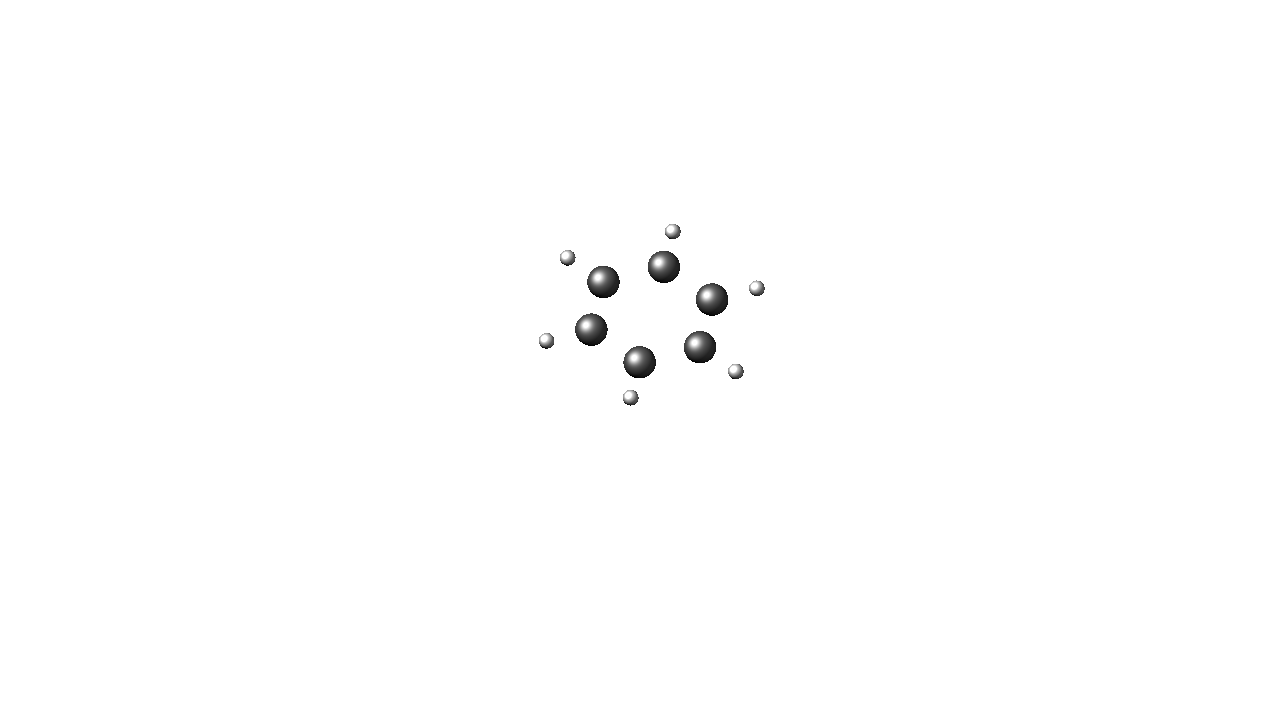
\includegraphics[width=0.40\textwidth]{c06h06}
    \bicaption{Q判据等值面图}
    \label{fig:c06h06}
\end{figure}

如果插图的空白区域过大,以图片\verb|c06h06|为例,自动裁剪如图~\ref{fig:c06h06_trim}。
\begin{figure}[!htbp]
    \centering
    %trim option's parameter order: left bottom right top
    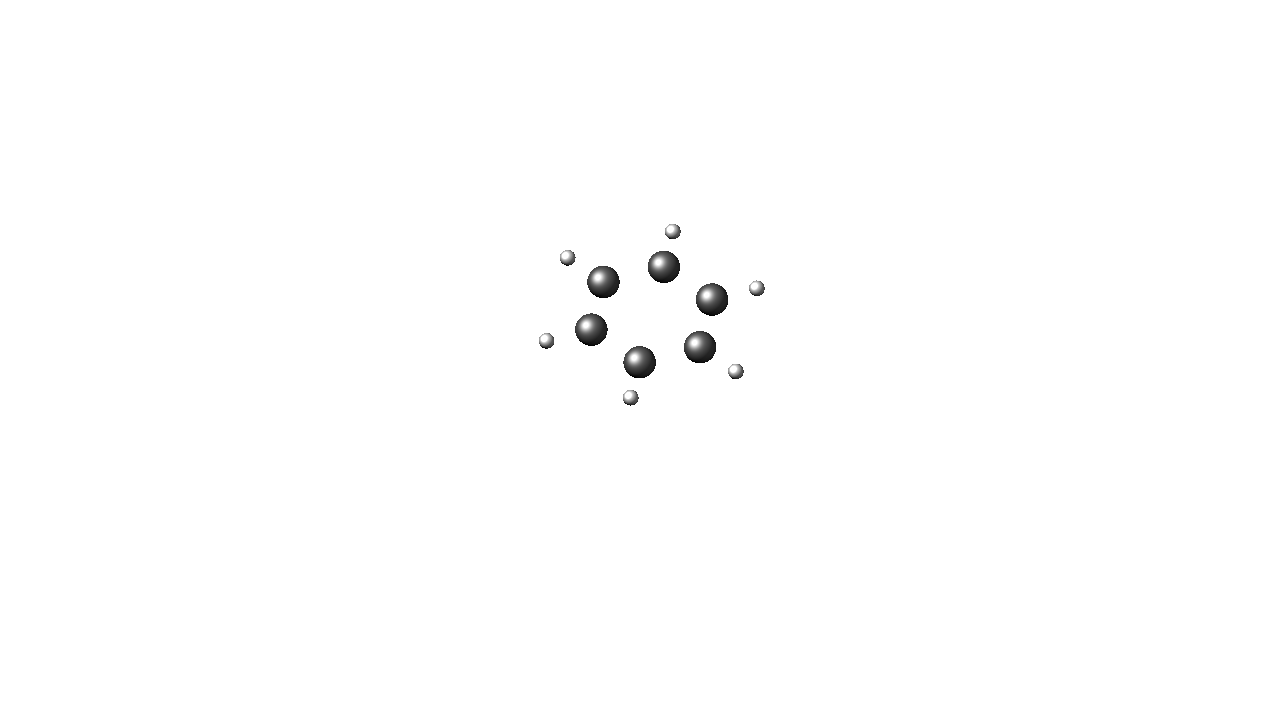
\includegraphics[trim = 60mm 80mm 60mm 60mm, clip, width=0.40\textwidth]{c06h06}
    \bicaption{激波圆柱作用。}{Shock-cylinder interaction.}
    \label{fig:c06h06_trim}
\end{figure}

多图的插入如图~\ref{fig:oaspl},多图不应在子图中给文本子标题,只要给序号,并在主标题中进行引用说明。
\begin{figure}[!htbp]
    \centering
    \begin{subfigure}[b]{0.35\textwidth}
      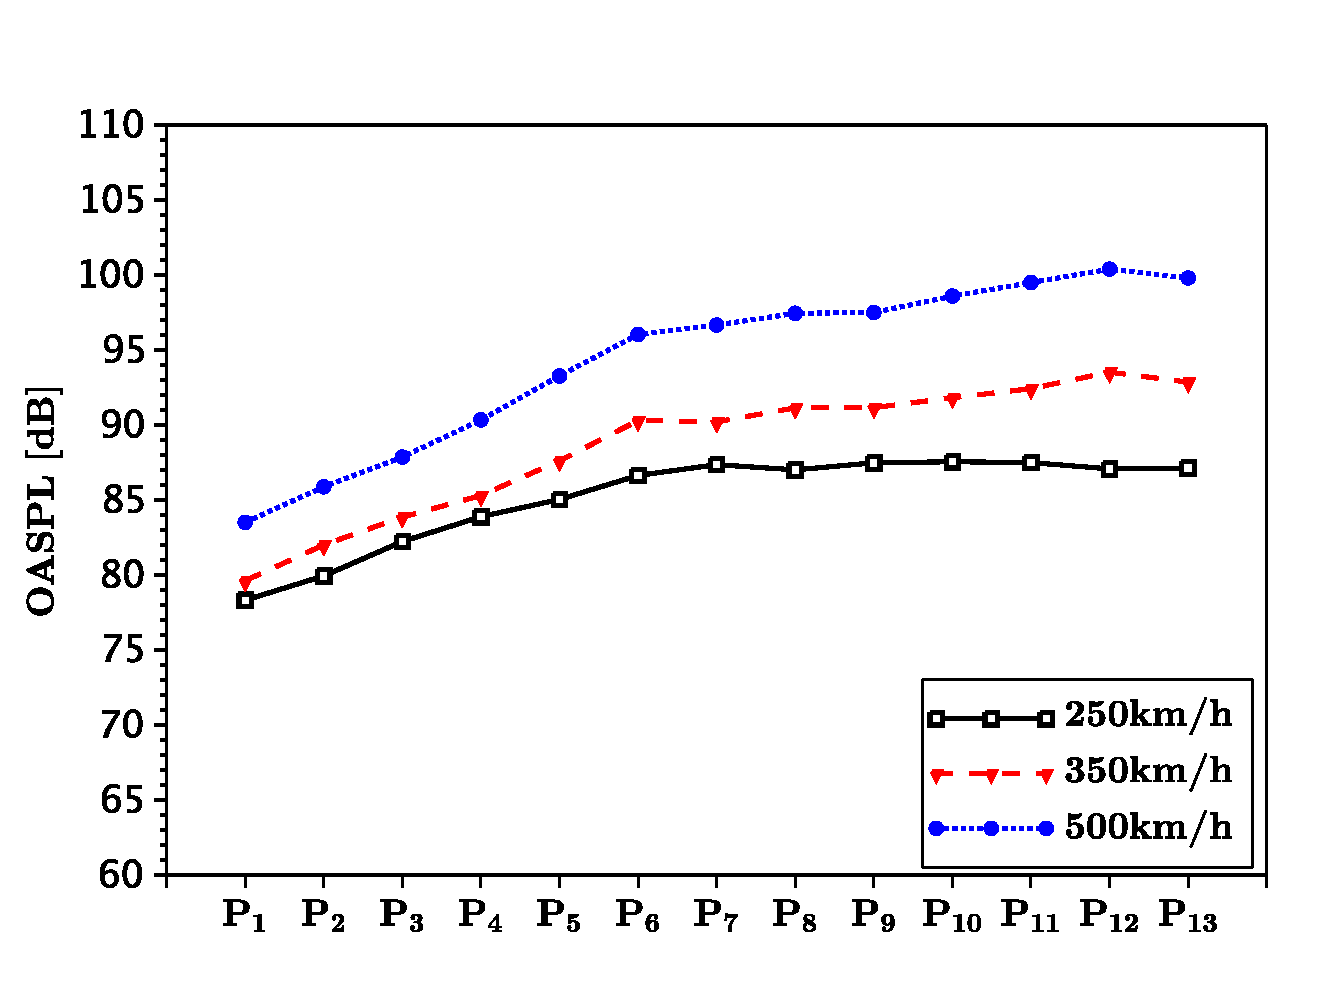
\includegraphics[width=\textwidth]{oaspl_a}
      \caption{}
      \label{fig:oaspl_a}
    \end{subfigure}%
    ~% add desired spacing
    \begin{subfigure}[b]{0.35\textwidth}
      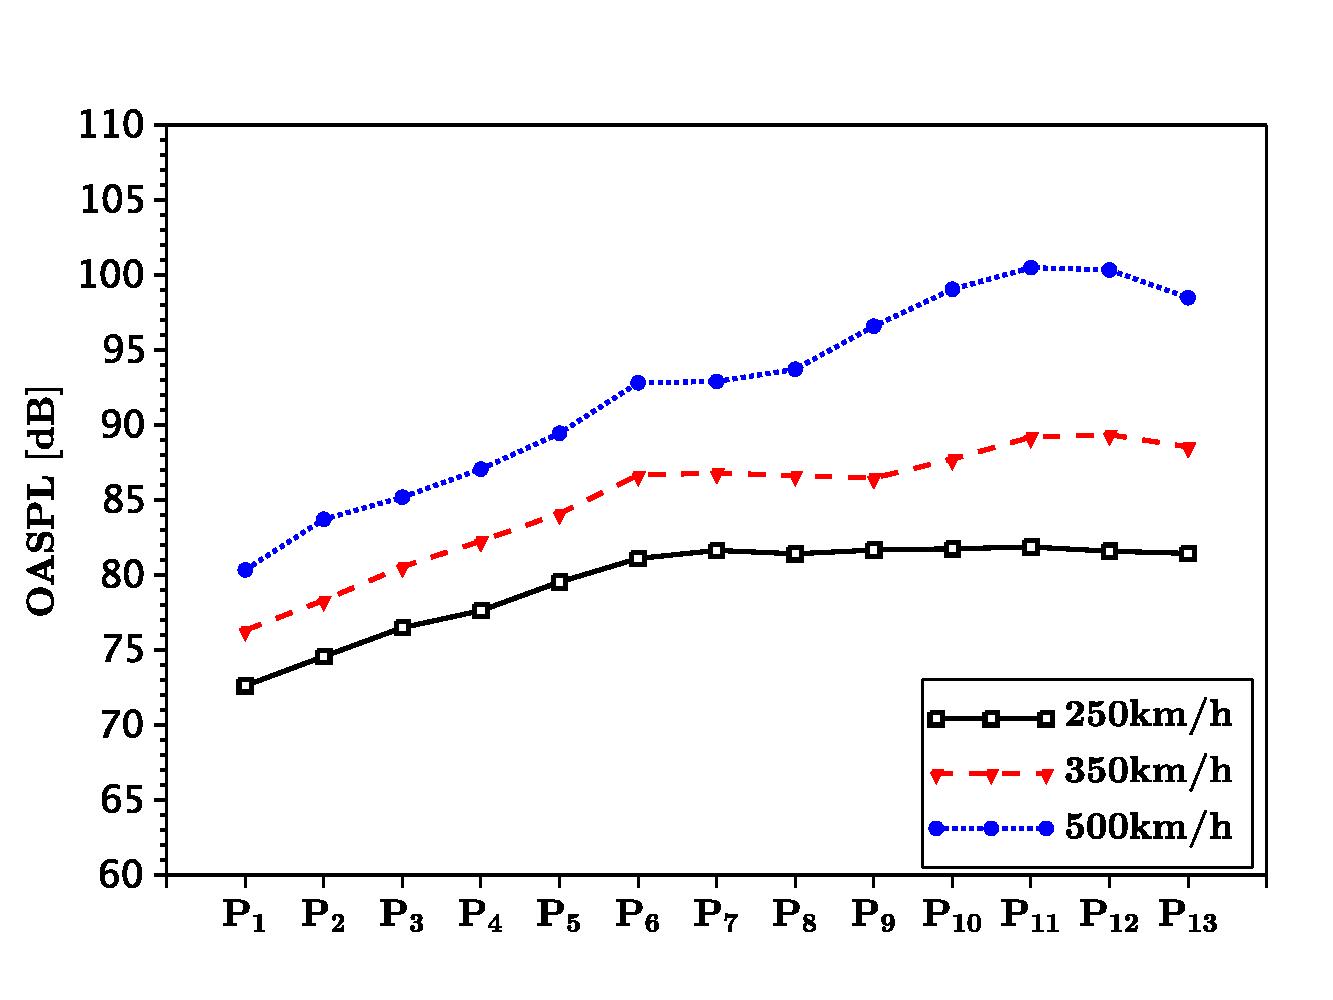
\includegraphics[width=\textwidth]{oaspl_b}
      \caption{}
      \label{fig:oaspl_b}
    \end{subfigure}
    \\% line break
    \begin{subfigure}[b]{0.35\textwidth}
      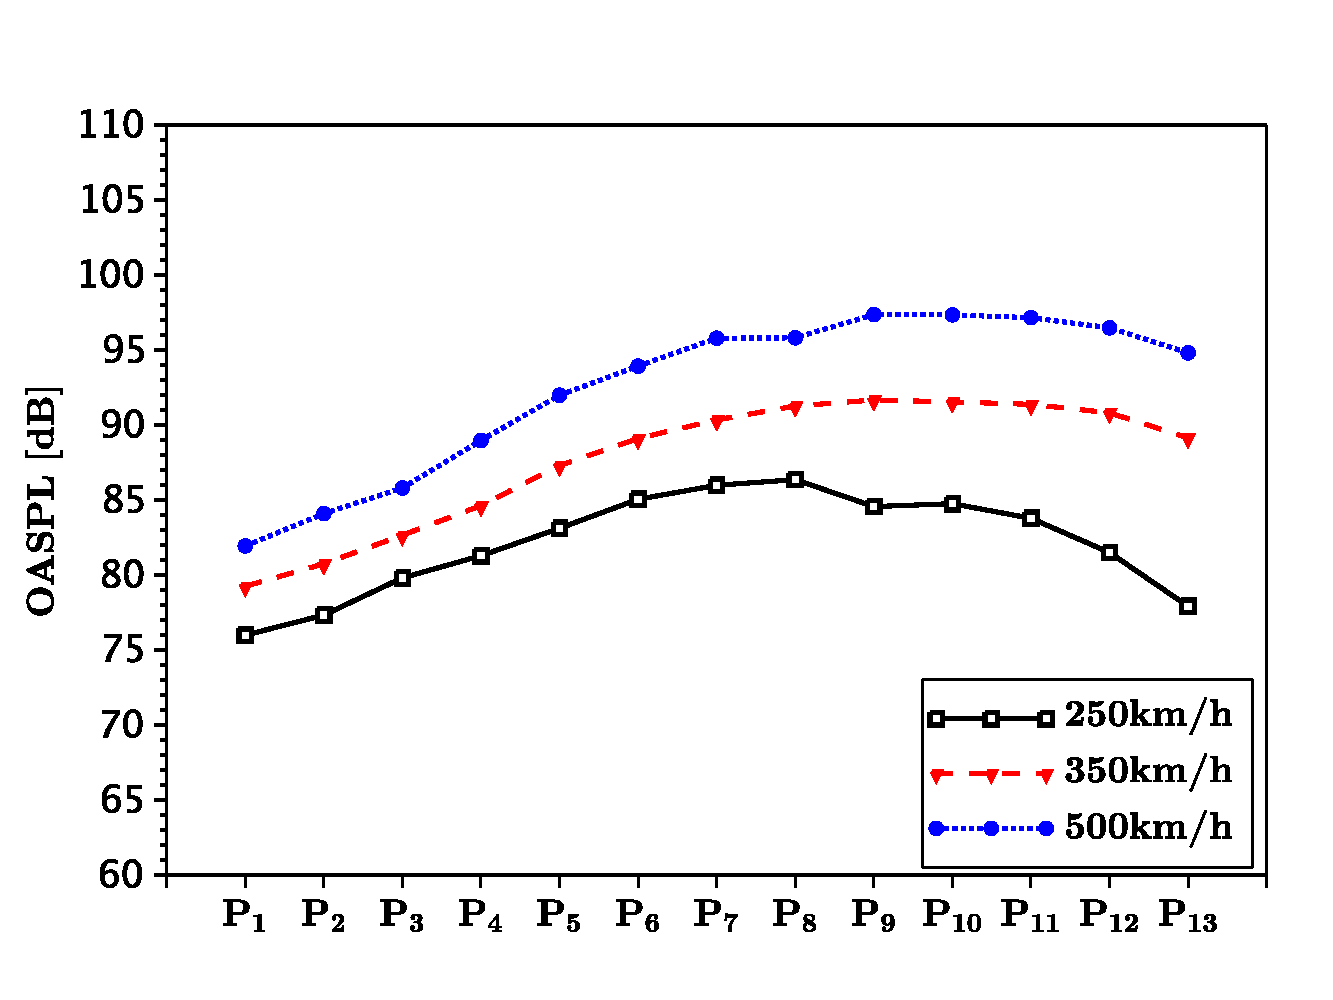
\includegraphics[width=\textwidth]{oaspl_c}
      \caption{}
      \label{fig:oaspl_c}
    \end{subfigure}%
    ~% add desired spacing
    \begin{subfigure}[b]{0.35\textwidth}
      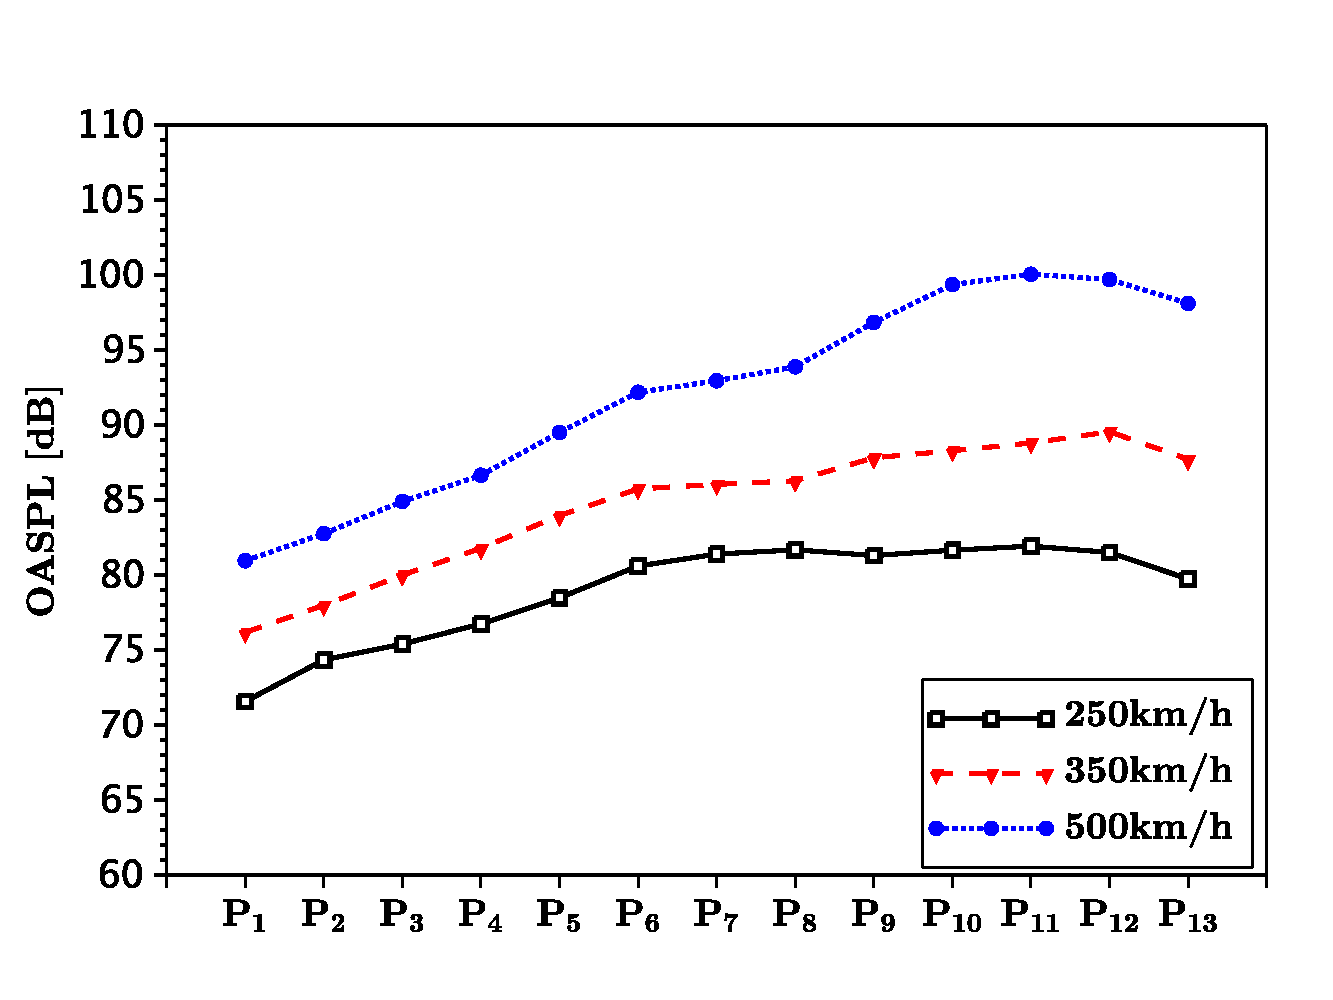
\includegraphics[width=\textwidth]{oaspl_d}
      \caption{}
      \label{fig:oaspl_d}
    \end{subfigure}
    \bicaption{总声压级。(a) 这是子图说明信息,(b) 这是子图说明信息,(c) 这是子图说明信息,(d) 这是子图说明信息。}{OASPL.(a) This is the explanation of subfig, (b) This is the explanation of subfig, (c) This is the explanation of subfig, (d) This is the explanation of subfig.}
    \label{fig:oaspl}
\end{figure}

\subsection{算法}

如见算法~\ref{alg:euclid},详细使用方法请参见文档 \href{https://ctan.org/pkg/algorithmicx?lang=en}{algorithmicx}。

\begin{algorithm}[!htbp]
    \small
    \caption{Euclid's algorithm}\label{alg:euclid}
    \begin{algorithmic}[1]
        \Procedure{Euclid}{$a,b$}\Comment{The g.c.d. of a and b}
        \State $r\gets a\bmod b$
        \While{$r\not=0$}\Comment{We have the answer if r is 0}
        \State $a\gets b$
        \State $b\gets r$
        \State $r\gets a\bmod b$
        \EndWhile\label{euclidendwhile}
        \State \textbf{return} $b$\Comment{The gcd is b}
        \EndProcedure
    \end{algorithmic}
\end{algorithm}

\subsection{参考文献引用}

参考文献引用过程以实例进行介绍,假设需要引用名为"Document Preparation System"的文献,步骤如下:

1)使用Google Scholar搜索Document Preparation System,在目标条目下点击Cite,展开后选择Import into BibTeX打开此文章的BibTeX索引信息,将它们copy添加到ref.bib文件中(此文件位于Biblio文件夹下)。

2)索引第一行 \verb|@article{lamport1986document,|中 \verb|lamport1986document| 即为此文献的label (\textbf{中文文献也必须使用英文label},一般遵照:姓氏拼音+年份+标题第一字拼音的格式),想要在论文中索引此文献,有两种索引类型:

文本类型:\verb|\citet{lamport1986document}|。正如此处所示 \citet{lamport1986document}; 

括号类型:\verb|\citep{lamport1986document}|。正如此处所示 \citep{lamport1986document}。

\textbf{多文献索引用英文逗号隔开}:

\verb|\citep{lamport1986document, chu2004tushu, chen2005zhulu}|。正如此处所示 \citep{lamport1986document, chu2004tushu, chen2005zhulu}

更多例子如:

\citet{walls2013drought} 根据 \citet{betts2005aging} 的研究,首次提出...。其中关于... \citep{walls2013drought, betts2005aging},是当前中国...得到迅速发展的研究领域 \citep{chen1980zhongguo, bravo1990comparative}。引用同一著者在同一年份出版的多篇文献时,在出版年份之后用
英文小写字母区别,如:\citep{yuan2012lana, yuan2012lanb, yuan2012lanc} 和 \citet{yuan2012lana, yuan2012lanb, yuan2012lanc}。同一处引用多篇文献时,按出版年份由近及远依次标注。例如 \citep{chen1980zhongguo, stamerjohanns2009mathml, hls2012jinji, niu2013zonghe}。

使用著者-出版年制(authoryear)式参考文献样式时,中文文献必须在BibTeX索引信息的 \textbf{key} 域(请参考ref.bib文件)填写作者姓名的拼音,才能使得文献列表按照拼音排序。参考文献表中的条目(不排序号),先按语种分类排列,语种顺 序是:中文、日文、英文、俄文、其他文种。然后,中文按汉语拼音字母顺序排列,日文按第一著者的姓氏笔画排序,西文和 俄文按第一著者姓氏首字母顺序排列。如中 \citep{niu2013zonghe}、日 \citep{Bohan1928}、英 \citep{stamerjohanns2009mathml}、俄 \citep{Dubrovin1906}。

如此,即完成了文献的索引,请查看下本文档的参考文献一章,看看是不是就是这么简单呢?是的,就是这么简单!

不同文献样式和引用样式,如著者-出版年制(authoryear)、顺序编码制(numbers)、上标顺序编码制(super)可在Thesis.tex中对artratex.sty调用实现,详见 \href{https://github.com/mohuangrui/ucasthesis/wiki}{ucasthesis 知识小站之文献样式}

%若在上标顺序编码制(super)模式下,希望在特定位置将上标改为嵌入式标,可使用 \citetns{niu2013zonghe,stamerjohanns2009mathml} 和 \citepns{niu2013zonghe,stamerjohanns2009mathml}。

参考文献索引的更多知识,请见 \href{https://en.wikibooks.org/wiki/LaTeX/Bibliography_Management}{WiKibook Bibliography}。\nocite{*}% 使文献列表显示所有参考文献(包括未引用文献)

\section{常见使用问题}\label{sec:qa}

\begin{enumerate}
    \item 模板每次发布前,都已在Windows,Linux,MacOS系统上测试通过。下载模板后,若编译出现错误,则请见 \href{https://github.com/mohuangrui/ucasthesis/wiki}{ucasthesis知识小站} 的 \href{https://github.com/mohuangrui/ucasthesis/wiki/%E7%BC%96%E8%AF%91%E6%8C%87%E5%8D%97}{编译指南}。

    \item 模板文档的编码为UTF-8编码。所有文件都必须采用UTF-8编码,否则编译后生成的文档将出现乱码文本。若出现文本编辑器无法打开文档或打开文档乱码的问题,请检查编辑器对UTF-8编码的支持。如果使用WinEdt作为文本编辑器(\textbf{不推荐使用}),应在其Options -> Preferences -> wrapping选项卡下将两种Wrapping Modes中的内容:
        
        TeX;HTML;ANSI;ASCII|DTX...
        
        修改为:TeX;\textbf{UTF-8|ACP;}HTML;ANSI;ASCII|DTX...
        
        同时,取消Options -> Preferences -> Unicode中的Enable ANSI Format。

    \item 推荐选择xelatex或lualatex编译引擎编译中文文档。编译脚本的默认设定为xelatex编译引擎。你也可以选择不使用脚本编译,如直接使用 \LaTeX{}文本编辑器编译。注:\LaTeX{}文本编辑器编译的默认设定为pdflatex编译引擎,若选择xelatex或lualatex编译引擎,请进入下拉菜单选择。为正确生成引用链接和参考文献,需要进行\textbf{全编译}。

    \item Texmaker使用简介
        \begin{enumerate}
            \footnotesize
            \item 使用 Texmaker “打开 (Open)” Thesis.tex。
            \item 菜单 “选项 (Options)” -> “设置当前文档为主文档 (Define as Master Document)”
            \item 菜单 “自定义 (User)” -> “自定义命令 (User Commands)” -> “编辑自定义命令 (Edit User Commands)” -> 左侧选择 “command 1”,右侧 “菜单项 (Menu Item)” 填入 Auto Build -> 点击下方“向导 (Wizard)” -> “添加 (Add)”: xelatex + bibtex + xelatex + xelatex + pdf viewer -> 点击“完成 (OK)”
            \item 使用 Auto Build 编译带有未生成引用链接的源文件,可以仅使用 xelatex 编译带有已经正确生成引用链接的源文件。
            \item 编译完成,“查看(View)” PDF,在PDF中 “ctrl+click” 可链接到相对应的源文件。
        \end{enumerate}
    
    \item 模版的设计可能地考虑了适应性。致谢等所有条目都是通过最为通用的

        \verb+\chapter{item name}+  and \verb+\section*{item name}+

        来显式实现的 (请观察Backmatter.tex),从而可以随意添加,放置,和修改,如同一般章节。对于图表目录名称则可在ucasthesis.cfg中进行修改。

    \item 设置文档样式: 在artratex.sty中搜索关键字定位相应命令,然后修改
        \begin{enumerate}
            \item 正文行距:启用和设置 \verb|\linespread{1.5}|,默认1.5倍行距。
            \item 参考文献行距:修改 \verb|\setlength{\bibsep}{0.0ex}|
            \item 目录显示级数:修改 \verb|\setcounter{tocdepth}{2}|
            \item 文档超链接的颜色及其显示:修改 \verb|\hypersetup|
        \end{enumerate}

    \item 文档内字体切换方法:
        \begin{itemize}
            \item 宋体:国科大论文模板ucasthesis 或 \textrm{国科大论文模板ucasthesis}
            \item 粗宋体:{\bfseries 国科大论文模板ucasthesis} 或 \textbf{国科大论文模板ucasthesis}
            \item 黑体:{\sffamily 国科大论文模板ucasthesis} 或 \textsf{国科大论文模板ucasthesis}
            \item 粗黑体:{\bfseries\sffamily 国科大论文模板ucasthesis} 或 \textsf{\bfseries 国科大论文模板ucasthesis}
            \item 仿宋:{\ttfamily 国科大论文模板ucasthesis} 或 \texttt{国科大论文模板ucasthesis}
            \item 粗仿宋:{\bfseries\ttfamily 国科大论文模板ucasthesis} 或 \texttt{\bfseries 国科大论文模板ucasthesis}
            \item 楷体:{\itshape 国科大论文模板ucasthesis} 或 \textit{国科大论文模板ucasthesis}
            \item 粗楷体:{\bfseries\itshape 国科大论文模板ucasthesis} 或 \textit{\bfseries 国科大论文模板ucasthesis}
        \end{itemize}
\end{enumerate}



\chapter{绪论}
\section{研究背景及意义}
从20世纪七八十年代开始,在国际上形成了非线性科学和复杂性问题的研究热潮。许多复杂性问题都可以从复杂网络的角度去研究。
钱学森将具有自组织、自相似、吸引子、小世界、无标度中部分或全部性质的网络统称为复杂网络。
原则上,任何包含大量组成单元(或子系统)的复杂系统,当我们把构成单元抽象成节点,单元之间的相互作用抽象为边时,都可以当作复杂网络来对其进行研究。
早期对复杂网络的研究主要集中在规则网络或完全随机网络上。
不过,规则网络和完全随机网络都是理想化的模型,而现实世界中的系统往往没有这么理想化,
很可能是有序和无序之间的网络(称为小世界网络)。早在1998年,Watts及Strogatz教授提出了经典的WS小世界网络,
该网络在规则网络基础上将每条边以概率p进行断边重连后得到。
小世界网络中含有大量的局部连边,同时也有少量长程连边,而这些长程连边有效地降低了网络中任意两个节点之间的距离,
这正是小世界特性的来源。
\section{研究现状}
最早的小世界网络动力学研究在1998年Watts及Strogatz的文章中给出,作者利用相应的小世界模型模拟传染病在人群中传播,
研究表明相较于规则网络,小世界网络的传播能力明显要快得多。2001年,Zhuo Gao研究了小世界网络的随机共振现象,
发现小世界网络的随机共振效应相比与普通网络有所增强。2002年,H. Hong等探讨了小世界网络同步性并发现随着重连概率的增大,
小世界网络中各个振子间同步性显著提高。2001年,Xin-She Yang对一个非线性时滞混沌小世界网络进行研究,
发现小世界混沌网络的传播要比规则网络速度更快。2012年,
Li Ning提出了一个基于小世界网络的离散复杂网络,并研究其分叉和混沌等动力学特性后发现相较于规则网络,
小世界网络的混沌现象在适当的参数下会得到控制。

此外,混沌信号由于其类噪声特性和长期不可预测性,已被广泛研究并用于保密通信、雷达信号处理、信号检测等诸多领域。
但在实际情况下,混沌信号总是会被噪声污染,而混沌信号具有非周期、宽带频谱等特性,一些现有的信号复原方法在处理混沌信号时难以获得理想的效果。
因此,研究噪声污染下混沌信号的重构技术具有重要意义,有效的混沌重构技术也将大大提高各种应用的性能。以压缩感知为典型代表的稀疏理论提出:
稀疏的或具有稀疏表达的有限维数的信号可以利用远少于奈奎斯特采样数量的线性、非自适应的测量值无失真地重建出来。
该理论一经提出,便在信息论、信号/图像处理、医疗成像、射电天文、模式识别、光学/雷达成像和信道编码等诸多领域引起广泛关注。
在信号处理领域,信号的稀疏重构理论仍是一个较新的研究方向,
近年来,学者们在该方向已取得了一些显著的研究成功,但很多问题仍需进一步研究。事实上,该理论的应用前提是能够对需处理的信号进行直接或间接的稀疏建模, 
合理地选取具有等距约束等限制条件的采样矩阵以及提出更高精度、更低复杂度或对噪声更鲁棒的后端恢复算法。
而能否将稀疏理论用于复杂系统带噪混沌信号的重构也是一个非常值得探讨的问题。

以压缩感知为典型代表的稀疏重构理论是一个较新的研究方向,一经提出便在信息论、信号/图像处理、医疗成像、射电天文、模式识别、光学/雷达成像和信道编码等诸多领域引起广泛关注[12,13]。
稀疏理论的应用前提是能够对信号进行直接或间接的稀疏化, 合理地选取具有等距约束等限制条件的采样矩阵以及提出高精度、低复杂度和抗噪声的重构算法[14]。
含噪混沌信号的稀疏重构问题尚未有完善的研究。因此,能否将稀疏理论用于复杂网络带噪混沌信号的重构具有重要意义,有效的混沌重构算法也将大大提高混沌信号各种应用的性能。
\section{本文主要工作和论文结构}
本文提出一个以WS小世界网络方式进行连接的Duffing复杂网络(简称Duffing-WS型小世界网络),并研究该复杂小世界网络的混沌现象,分析复杂系统耦合强度、重连概率、邻接度等参数对其混沌特性的影响规律;同时考虑采用稀疏重构理论建立重构算法还原小世界网络生成的带噪混沌信号。
利用变分法推导Duffing-WS型小世界网络的最大李雅普诺夫指数表达式,以庞加莱截面分岔图和李雅普诺夫指数为工具研究该复杂网络的混沌现象,通过微分方程数值解法进行数值仿真,使用LE指数衡量系统的混沌程度与振幅范围,分析小世界网络重连度,重连概率和耦合强度对此复杂网络混沌现象的影响。
现有文献主要研究复杂网络的同步、传播和共振等动力学特性,对复杂网络的混沌研究较少。本文针对一个以WS小世界网络方式进行连接的Duffing复杂网络,研究其混沌特性,并基于优异的并行处理计算架构相应的数值仿真算法分析各个参数对混沌的影响。
已针对研究领域进行了必要的理论调研和学习了相关基础理论,针对提出的模型利用变分法推导Duffing-WS型小世界网络的最大李雅普诺夫指数表达式;此外具有并行处理能力的计算机,高性能程序开发经验,能够基于优异的并行处理计算架构给出相应的数值仿真算法。
理清耦合强度、重连概率、邻接度等参数的变化对系统混沌的影响,找到控制复杂网络混沌现象的关键;基于稀疏理论给出复杂系统带噪混沌信号的重构算法。

\chapter{基础理论}
\section{复杂网络基本概念}
复杂网络科学与工程重点研究自然科学技术和社会政治经济中各种复杂系统微观性态与宏观现象之间的密切联系,特别是其网络结构的形成机理与演化方式、
结构模式与动态行为、运动规律与调控策略,以及多关联复杂系统在不同尺度下行为之间的相关性等。网络科学与工程融合了数学、统计物理、计算机科学及各类工程技术科学,
探索采用复杂系统自组织演化发展的思想去建立全新的理论和方法,其中的网络拓扑学拓展了人们对复杂系统的认识,而网络动力学则更深入地刻画了复杂系统的本质。
网络科学既是数学中经典图论和随机图论的自然延伸,也是系统科学和复杂性科学的创新发展。\par

图论是一种强有力的研究工具和研究方法。图(Graph)提供了一种用抽象的点和线表示各种实际网络的统一方法,因而也成为目前研究复杂网络的一种共同的语言。
下面我们给出图论的几个基本概念。
\subsection{图论的基本知识}
图是对系统中基本单元(称为节点)集合,以及每两个基本单元之间关系(边)集合之间关系的描述。图可以定义为一个三元组$G=(V,E,\phi)$
集合$V=\{v_1,v_2,…,v_n\}$称为节点集;
集合$E=\{e_1,e_2,…,e_m\}$称为边集;

$\phi$是边集E到节点集V的一个映射,称为关联函数。
V中的元素称为节点或顶点(node或vertex), E中的元素称为边、弧或连线(edge,arc或line),且E中的每条边em都有V的一对节点$(v_i,v_j)$与之对应。
用计算机分析实际网络的性质面临的第一个问题就是如何在计算机中表示一个网络。图的矩阵表示架起了图论与矩阵论之间的桥梁,通过这种表示方法就能借助于矩阵的理论和分析方法来研究图论中的问题。
邻接矩阵描述了节点与节点之间的邻接关系,通常会用一个方阵A来表示,方阵中的元素用$a_{ij}$表示。          

记$G=(V,E)$为一个非空图,其中$V$是其顶点集,$E$是边集。图中一点$v$的相邻点集记为$N(v)$,顶点的度是指与其相连的边的个数
记为$d(v)$,一个图的平均度定义为
\begin{equation}
    d(G):=\frac{1}{|V|} \sum_{v \in V} d(v)
\end{equation}
图$G$的一条路径是一个子图,其顶点集与边集描述了原图中某一点到另一点的一条通路。一个圈是指一个子图,描述了以某点为起始点与终止点
的一条非平凡路径。
一个含有$N$个节点、$M$个边的图$G$的密度定义$\rho$为
\begin{equation}
    \rho=\frac{M}{\frac{1}{2} N(N-1)}
\end{equation}
\begin{definition}
    如果非空图$G$中任意两顶点之间均有一条路相连,称图$G$为联通图。
\end{definition}
给定子图 $A,B \subseteq V$ 和 $X \subseteq V \cup E$,如果 $G$ 的每条 $A-B$ 路均包含 $X$ 中的一个顶点或一条边,
称在 $G$ 中 $X$ 分离 (separate) 集合 $A$ 和 $B$ 。
下面是图论中一个重要的定理。
\begin{theorem}
    设 $G=(V,E)$ 是一个图且 $A,B \subseteq V$ 。那么,在$G$ 中分离 $A$ 和 $B$ 的顶点的最小数目等于 $G$ 中互不
    相交的 $A-B$ 路的最大数目。
\end{theorem}
网络中节点的距离定义为连接这两个点的最小所经边数目。网络的平均长度定义为
\begin{equation}
    L=\frac{1}{\frac{1}{2} N(N-1)} \sum_{i \neq j} d_{i j}
\end{equation}
其中$d_{ij}$为节点$i,j$之间的距离。如果图本身并不联通,则只计算相连两点的距离的算术平均数。
一个图的直径$D$定义为任意两个节点之间距离的最大值。
\begin{definition}
    图中一个节点$i$的聚类系数$C_i$定义为
\begin{equation}
    C_i=\frac{E_i}{\left(k_i\left(k_i-1\right)\right) / 2}=\frac{2 E_i}{k_i\left(k_i-1\right)}
\end{equation}
其中$k_i$为该节点的度,$E_i$为其$k_i$个邻节点之间存在的边的数目。
还有一种聚类系数的几何定义,两个定义并不等价,一般会加以说明
\begin{equation}
    C_i=\frac{\text { 包含节点 } i \text { 的三角形的数目 }}{\text { 以节点 } i \text { 为中心的连通三元组的数目 }}
\end{equation}
\end{definition}
图的聚类系数定义为节点的聚类系数的均值
\begin{equation}
    C=\frac{1}{N} \sum_{i=1}^N C_i
\end{equation}
\subsection{规则网络}
如果系统中节点及其与边的关系是固定的,每个节点都有相同的度数,就可以用规则图来表示这个系统。这样的网络就称为规则网络。
常见的规则网络包括:全局耦合网络、最近邻耦合网络和星形耦合网络等。他们的结构示意图如下:
\begin{figure}[!htbp]
    \centering
    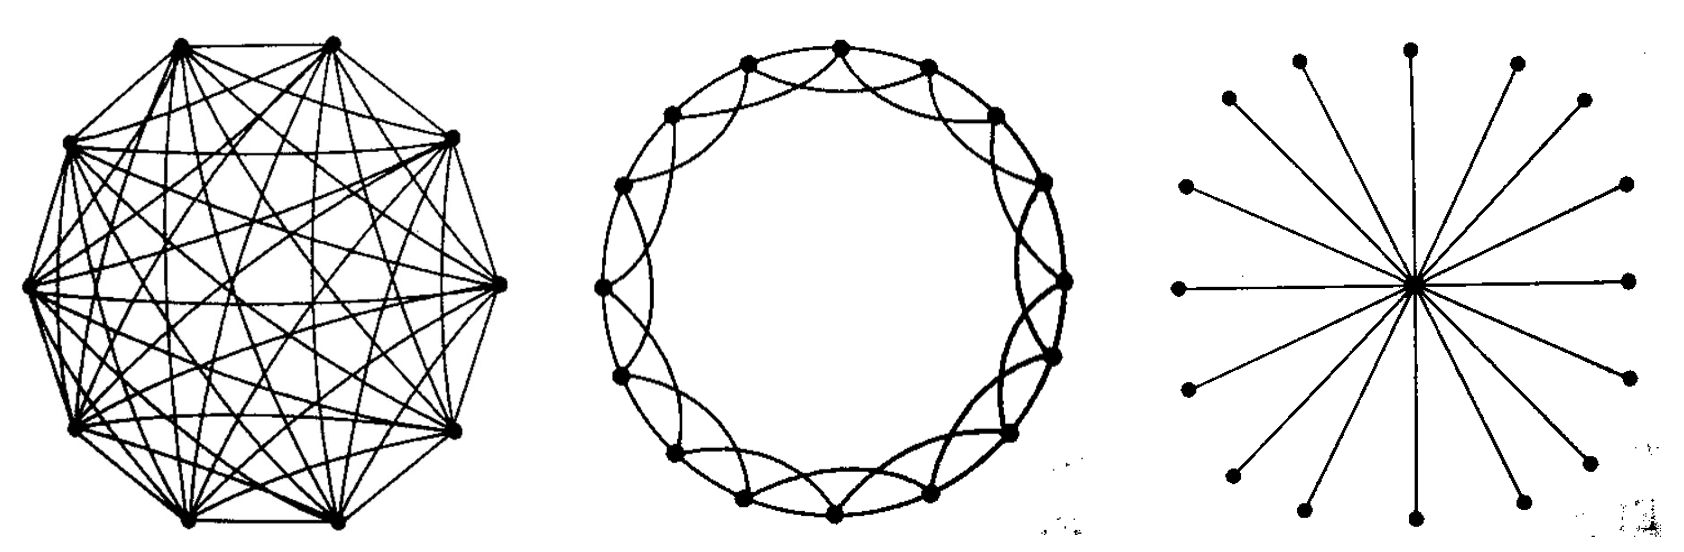
\includegraphics[width=0.8\textwidth]{guize.png}
    \caption{规则网络}
\end{figure}

\subsection{复杂网络}
系统是由相互作用和相互依赖的若干组成部分结合的具有特定功能的有机整体。从三个方面理解系统的概念:
     ①系统是由若干要素(部分)组成的。
     ②系统有一定的结构。
     ③系统有一定的功能。
     系统有如下的属性:
     集合性、相关性、层次性、整体性、涌现性、对环境的适应性
从图论意义上理解网络,网络是指由节点和连线构成的图。有时用带箭头的连线表示从一个节点到另一个节点存在的某种顺序关系。有时在节点或连线旁标出数值,称为点权或线权,有时不标任何数。
网络和系统通常是密切联系的,如果用节点表示系统的各个组成部分即系统的元素,两个节点之间的连线表示系统元素之间的相互作用,那么网络就为研究系统提供了一种新的描述方式。
一般认为复杂系统具有以下特征:非线性与动态性、非周期性和开放性、奇怪吸引性、结构自相似性(分形)。另外,复杂系统还具有突现性、不稳性、不确定性、不可预测性等特征。
复杂网络可以看作由一些具有独立特征的又与其他个体相互连接的节点的集合,每个个体可视为图中一个节点,节点间的相互连接视为图中的边。复杂网络包括两个层面:作为其连接拓扑结构的图和作为其状态和功能的系统。
\par 钱学森给出了复杂网络的一个较严格的定义:具有自组织、自相似、吸引子、小世界、无标度中部分或全部性质的网络称为复杂网络。
原则上说,任何包含大量组成单元(或子系统)的复杂系统,当我们把构成单元抽象成节点,单元之间的相互作用抽象为边时,都可以当作复杂网络来研究。

复杂网络是指不规则、度分布不均匀的网络模型,常见的复杂网络模型有全随机方式生成的ER随机图,在规则网络上进行修改的小世界模型。本节内容会给出
这几种的复杂网络模型的生成方法与其性质。
\subsubsection{ER随机图}
与完全规则网络相反的是完全随机网络。典型的模型是Erdös和Rényi于40多年前开始研究的ER随机图模型,其顶点采用完全随机连边的方式进行连接,它是一种完全随机图
,是随机性最强的图。下面我们首先给出具有固定次数连接独立两点的ER随机图$G(N,M)$的构造算法:\par 
\noindent(1) 初始化: 给定 $N$ 个节点和待添加的边数 $M$ 。\par
\noindent(2) 随机连边:\par
1) 随机选取一对没有边相连的不同的节点,并在这对节点之间添加一 条边。\par
2)重复步骤1),直至在 $M$ 对不同的节点对之间各添加了一条边。\par
然后给出以一定概率连接各独立顶点的ER 随机图 $G(N,p)$ 构造算法:\par
\noindent(1) 初始化: 给定 $N$ 个节点以及连边概率 $p \in[0,1]$ 。\par
\noindent(2) 随机连边:\par
1) 选择一对没有边相连的不同的节点。\par
2) 生成一个随机数 $r \in(0,1)$ 。\par
3) 如果 $r<p$,那么在这对节点之间添加一条边; 否则就不添加边。\par
4) 重复步骤1)-3),直至所有的节点对都被选择过一次。\par
对第二种$G(N,M)$进行性质分析。首先生成的随机图恰好具有 $M$ 条边的概率为
\begin{equation}
    P(M)=\left(\begin{array}{c}
    C^2_N \\
    M
    \end{array}\right) p^M(1-p)\left(\begin{array}{c}
    N \\
    2
    \end{array}\right)^{-M}
\end{equation}
其中,$C^2_N=\left(\begin{array}{c}
    N \\
    2
    \end{array}\right)$,
$\left(\begin{array}{c}
    C^2_N \\
    M
    \end{array}\right)$表示具有 $N$ 个节点和 $M$ 条边的简单图的数量,
    $p^M(1-p)^{C^2_N-M}$ 
表示有 $M$ 对节点之间添加了边, $C^2_N-M$ 对节点之间没有添加边。
边数分布的平均值为:
\begin{equation}
    \langle M\rangle=\sum_{n=0}^{C^2_N} M P(M)=\left(\begin{array}{l}
    N \\
    2
    \end{array}\right) p=p \frac{N(N-1)}{2}
    \end{equation}
边数分布的方差:
\begin{equation}
    \sigma_M^2=\left\langle M^2\right\rangle-\langle M\rangle^2=p(1-p) \frac{N(N-1)}{2}
\end{equation}
$G(N,M)$中节点度的概率分布符合泊松分布。
\begin{equation}
    P(k)=\left(\begin{array}{c}
    N-1 \\
    k
    \end{array}\right) p^k(1-p)^{N-1-k}
\end{equation}
根据概率统计中的内容,其期望与方差分别为
\begin{equation}
    \langle k\rangle=p(N-1)
\end{equation}
\begin{equation}
    \sigma_k^2=p(1-p)(N-1)
\end{equation}
由于两个节点之间不论是否具有共同的邻居节点,共连接概率均为$p$,所以聚类系数为
\begin{equation}
    C=p=\langle k\rangle /(N-1)
\end{equation}
\subsubsection{WS小世界模型}
WS小世界模型是通过在规则图上做带有随机性的更改形成的。下面给出WS模型构建算法如下:\par
\noindent(1) 从规则图开始: 给定一个含有 $N$ 个点的环状最近邻耦合网络,其中 每个节点都与它左右相邻的各 $K / 2$ 个节点相连,$K$ 是偶数。\par
\noindent(2) 随机化重连: 以概率 $p$ 随机地重新连接网络中原有的每条边,即把 每条边的一个端点保持不变,另一个端点改取为网络中随机选择的一个节点。
其中规定不得有重边和自环。\par
\begin{figure}[!htbp]
    \centering
    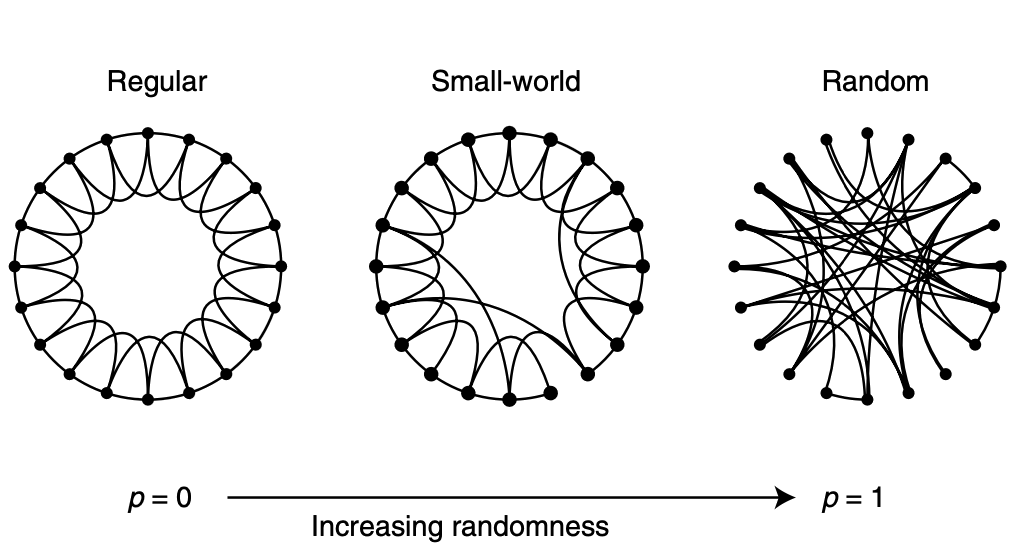
\includegraphics[width=0.8\textwidth]{wsp1.png}
    \caption{WS随机网络的构造}
\end{figure}
可以看出,$p=0$时是完全规则的网络,$p=1$时是完全随机的网络。WS模型的聚类系数与平均路径长度是关于重连概率$p$的函数,
其关系如下图\par
\begin{figure}[!htbp]
    \centering
    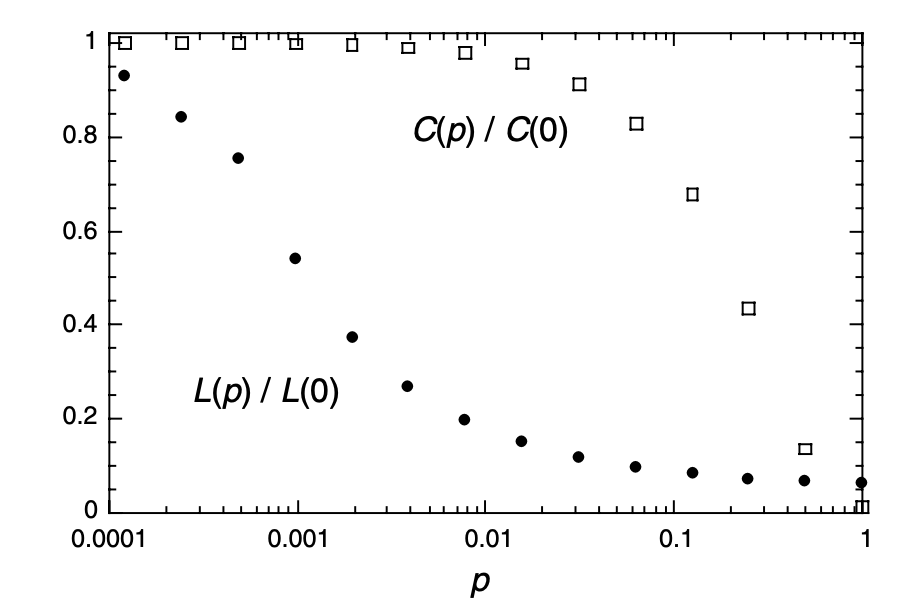
\includegraphics[width=0.8\textwidth]{WS.png}
    \caption{WS随机网络的聚类系数与重连概率}
\end{figure}
WS模型的聚类系数的估计如下
\begin{equation}
    \begin{aligned}
    \tilde{C}_{W S}(p) & \triangleq \frac{M_0(1-p)^3+O(1 / N)}{K(K-1) / 2} \\
    & =\frac{3 K(K-2) / 8}{K(K-1) / 2}(1-p)^3+O(1 / N) \\
    & =\frac{3(K-2)}{4(K-1)}(1-p)^3+O(1 / N) \\
    & =C_{n c}(1-p)^3+O(1 / N)
    \end{aligned}
\end{equation}\par
下面来研究WS模型的度分布,在 $p>0$ 时,每个节点仍与顺时针方向的 $K / 2$ 条原有的边相连,即每个节点的度至少为 $K / 2$ 。
 为此,记节点 $i$ 的度为 $k_i=s_i+K / 2$。 $s_i$ 又可分为两部分: 
 $s_i=s_i^1+s_i^2$,$s_i^1$ 表示在原有的与节点 $i$ 相连的逆时针方向的 $K / 2$ 条边中保持不变的边的数目,
 其中每条边不变的概率为 $1-p ; s_i^2$ 表示通过随机重连机制连接节点 $i$ 上的长程边,
 每条这样的边的概率 为 $p / N$ 。有
 \begin{equation}
    \begin{gathered}
    P_1\left(s_i^1\right)=\left(\begin{array}{c}
    K / 2 \\
    s_i^1
    \end{array}\right)(1-p)^{s_i^{1}} p^{K / 2-s_i^1}\\
    P_2\left(s_i^2\right) \simeq \frac{(p K / 2)^{s_i^2}}{\left(s_i^2\right) !} \mathrm{e}^{-\rho K / 2}\text { 当 } N \text { 充分大时. }
    \end{gathered}
\end{equation}
对于任一度为 $k \geqslant K / 2$ 的节点,$s_i^1 \in[0,\min (k-K / 2,K / 2)]$ 。
当$k<K/2$时,$P(k)=0$,当 $k \geqslant$ $K / 2$ 时
\begin{equation}
    P(k)=\sum_{n=0}^{\min (k-K / 2,K / 2)}\left(\begin{array}{c}
    K / 2 \\
    n
    \end{array}\right)(1-p)^n p^{K / 2-n} \frac{(p K / 2)^{k-(K / 2)-n}}{(k-(K / 2)-n) !} \mathrm{e}^{-p K / 2}
\end{equation}
\subsubsection{NW小世界模型}
NW小世界模型是通过在规则图上有随机性的增加长程边形成的,相比WS模型,这是一种更常见的小世界模型。
下面给出NW模型构建算法如下\par
\noindent(1) 从规则图开始: 给定一个含有 $N$ 个节点的环状最近邻耦合网络,其中每个节点都与它左右相邻的各 $K / 2$ 个节点相连,$K$ 是偶数。\par
\noindent(2) 随机化加边: 以概率 $p$ 在随机选取的 $NK / 2$ 对节点之间添加边,其中 规定不得有重边和自环。\par
首先讨论NW模型的聚类系数,NW模型的聚类系数采用几何聚类系数来讨论,$p=0$ 时,网络中的三角形数量为 
$\frac{1}{4} N K\left(\frac{1}{2} K-1\right)$。$ p>0$ 时,
现在我们需要计算在添加了长程边之后新增加的三角形的数量。 网络中长程边的平均数为 $\frac{1}{2} N K p$,
这些边可以在 $\frac{1}{2} N(N-1)$ 个点对之间添加,每一对节点之间有长程边相连的概率为
\begin{equation}
    \frac{\frac{1}{2} N K p}{\frac{1}{2} N(N-1)}=\frac{K p}{N-1} \approx \frac{K p}{N}
 \end{equation}
 包含一条长程边的三角形数量可以近似为一个与$N$无关的常数:
 \begin{equation}
    N \times \frac{K p}{N}=K p
\end{equation}
当网络规模趋于无穷时,这一常数与最近邻网络的三角形数量相比是可以忽略不计的。因此,对于 $0 \leqslant p \ll 1$ 
模型中的三角形的数量近似为 $\frac{1}{4} N K\left(\frac{1}{2} K-1\right) $
每条长程边都可以与$N$条边的两个端点之一形成连通三元组,因此包含一条长程边的连通三元组的平均数量为
\begin{equation}
    \frac{1}{2} N K p \times K \times 2=N K^2 p
\end{equation}
如果一个节点与 $m>1$ 条长程边相连,那么从中任选两条长程边就构成一个 连通三元组,共有 $\frac{1}{2} m(m-1)$ 种可能。
平均一个节点与 $K p$ 条长程边相连,因此 网络中以一个节点为中心的包含两条长程边的连通三元组数量的均值为
\begin{equation}
    N \times \frac{1}{2} K p(K p-1) \approx \frac{1}{2} N K^2 p^2
\end{equation}
因此,NW模型中总的连通三元组的数量的均值为
\begin{equation}
    \frac{1}{2} N K(K-1)+N K^2 p+\frac{1}{2} N K^2 p^2
\end{equation}
综上所述,当$0 \leqslant p<1$时,NW小世界网络模型的聚类系数的估计值为
\begin{equation}
    \begin{aligned}
    \tilde{C}_{N W}(p) & =\frac{3 \times \frac{1}{4} N K\left(\frac{1}{2} K-1\right)}{\frac{1}{2} N K(K-1)+N K^2 p+\frac{1}{2} N K^2 p^2} \\
    & =\frac{3(K-2)}{4(K-1)+4 K p(p+2)} 
    \end{aligned}
\end{equation}
小世界模型的平均路径长度具有如下形式
\begin{equation}
    L=\frac{N}{K} f(N K p)
\end{equation}
$f(x)$被称为普适标度函数,NW模型的平均路径长度有如下近似
\begin{equation}
    f(x)=\frac{2}{\sqrt{x^2+4 x}} \operatorname{artanh} \sqrt{\frac{x}{x+4}}
\end{equation}
在$x$远大于1时,可以简化为
\begin{equation}
    f(x) \simeq \frac{1}{\sqrt{x^2+4 x}} \ln \frac{\sqrt{1+4 / x}+1}{\sqrt{1+4 / x}-1} \simeq \frac{\ln x}{x},\quad x>>1
\end{equation}
将$f(x)$代入,最后得出
\begin{equation}
    L=\frac{\ln (N K p)}{K^2 p},\quad N K p>>1
\end{equation}
由图看出,这种近似效果优异。\par
\begin{figure}[!htbp]
    \centering
    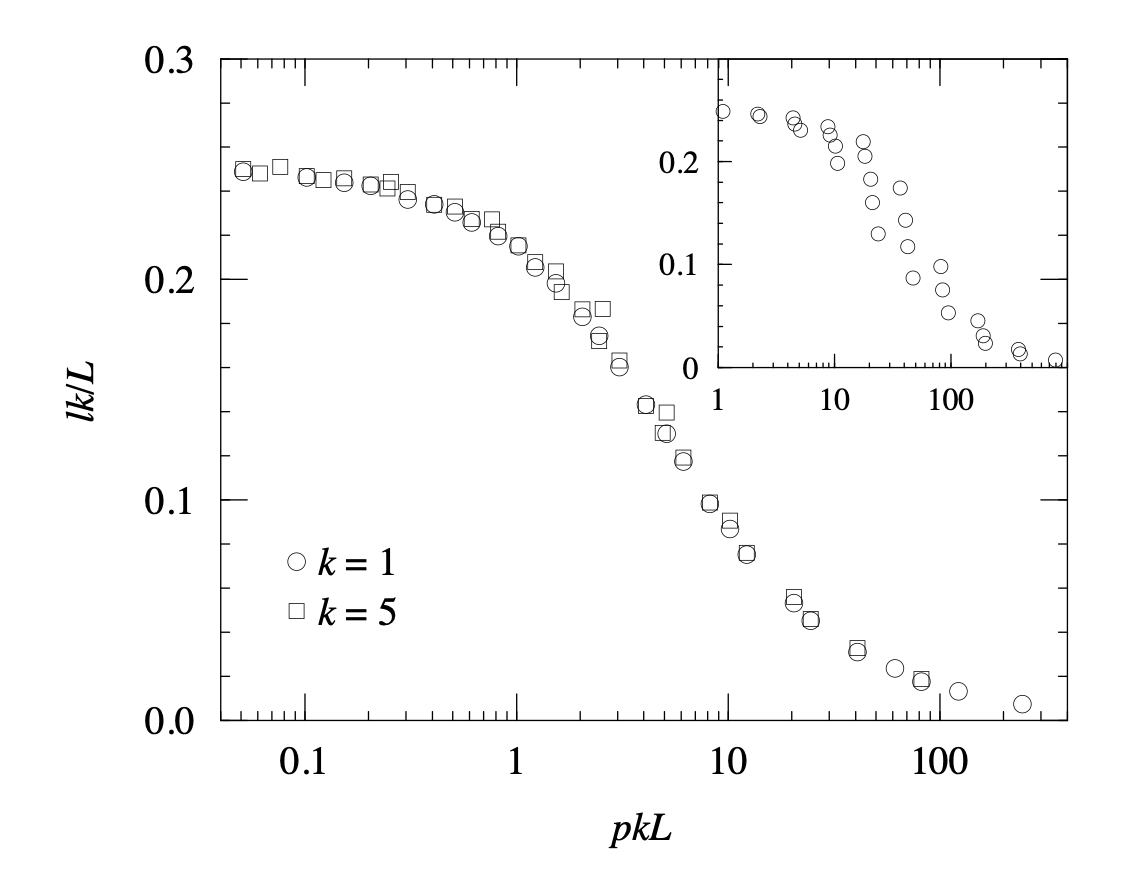
\includegraphics[width=0.8\textwidth]{NW1.png}
    \caption{NW随机网络的平均路径长度}
\end{figure}
下面讨论度分布,由于每对节点之间有边相连的概率为 $Kp/(N-1)$,因此
\begin{equation}
    P(k)=\left(\begin{array}{l}
    N-1 \\
    k-K
    \end{array}\right)\left[\frac{K p}{N-1}\right]^{k-K}\left[1-\frac{K p}{N-1}\right]^{N-1-k+K}
\end{equation}
NW模型中长程边的平均数为 $\frac{1}{2} N K p$,涉及的端点数目为 $N K p$ 。
因此,网络中长程边的数量为 $K p$,
即 $\langle k-K\rangle=K p$ 。当网络中节点数 $N$ 充分大时,可近似写为泊松分布:
\begin{equation}
    P(k)=\frac{(K p)^{k-K}}{(k-K) !} \mathrm{e}^{-K_p}
\end{equation}
\section{非线性系统的稳定性和混沌}
在刘慈欣的著作《三体》中提到了一个经典的天体物理问题——三体问题,这个问题的一个重要特点是三体系统的不稳定性,即在微小扰动的影响下,
依托于一定时间内已知的位置与运动信息预测出将来的位置具有很大的变化。现实中很难把握系统中全部的微信息,例如一个原子的微小扰动几乎是
难以描述的,如果模型自身对这种微小差异敏感度极高,那意味着这个系统几乎没有可以预测的可能性,预测出的结果与现实差异会随着时间轴指数级放大。
衡量非线性系统的稳定性研究主要由李雅普诺夫稳定性入手。
\subsection{非线性系统的稳定性}
考虑自治系统
\begin{equation}
    \dot{x}=f(x)
\end{equation}
其中 $,f: D \rightarrow R^n$ 是从定义域 $D \subset R^n$ 到 $R^n$ 上的局部利普希茨映射。
假定 $\bar{x} \in D$ 是其平衡点,即 $f(\bar{x})=0$ 。不失一般性,所有定义和定理都是对平衡点在 $R^n$ 上的原点,
即 $\bar{x}=0$ 时的情况而言。因为经过变量代换总可以把平衡点变换为原点。假设 $\bar{x} \neq 0$,经 $y=x-\bar{x}$ 变换后,$y$ 的
导数为
\begin{equation}
    \dot{y}=\dot{x}=f(x)=f(y+\bar{x}) \stackrel{\text { def }}{=} g(y),g(0)=0
\end{equation}
对于变量$y$,系统在原点有平衡点。
\begin{definition}
    对于平衡点$x=0$,如果对于每个 $\varepsilon>0$,都存在 $\delta=\delta(\varepsilon)>0$, 满足
    \begin{equation}
        \|x(0)\|<\delta \Rightarrow\|x(t)\|<\varepsilon,\quad \forall t \geqslant 0
    \end{equation}
    则该平衡,点是稳定的。
    如果稳定,且可选择适当的 $\delta$, 满足
    \begin{equation}
        \|x(0)\|<\delta \Rightarrow \lim _{t \rightarrow \infty} x(t)=0
    \end{equation}
    则该平衡,点是渐近稳定的。
\end{definition}
下面的李雅普诺夫稳定性定理是判断平衡点稳定的重要方法,它能够用某些其他函数代替能量以确定平衡点的稳定性。
设 $V: D \rightarrow R$ 是连续可微函数,$\dot{V}(x)$是$V(x)$沿方程轨线的导数。即
\begin{equation}
    \begin{aligned}
    \dot{V}(x) & =\sum_{i=1}^n \frac{\partial V}{\partial x_i} \dot{x}_i=\sum_{i=1}^n \frac{\partial V}{\partial x_i} f_i(x) \\
    & =\left[\begin{array}{llll}
    \frac{\partial V}{\partial x_1},& \frac{\partial V}{\partial x_2},& \cdots,& \frac{\partial V}{\partial x_n}
    \end{array}\right]\left[\begin{array}{c}
    f_1(x) \\
    f_2(x) \\
    \vdots \\
    f_n(x)
    \end{array}\right]=\frac{\partial V}{\partial x} f(x)
    \end{aligned}
\end{equation}
\begin{theorem}
    设 $x=0$ 是方程的一个平衡点,$D \subset R^n$ 是包含原点的定义域。设 $V: D \rightarrow R$ 是连续可微函数,如果
    \begin{equation}
        \begin{array}{lll}
        V(0)=0,& V(x)>0 & \text { 在 } D-\{0\} \text { 内 } \\
        & \dot{V}(x) \leqslant 0 & \text { 在 } D \text { 内 }
        \end{array}
    \end{equation}
    那么,原点 $x=0$ 是稳定的。此外,如果
    \begin{equation}
        \dot{V}(x)<0 \quad \text { 在 } D-\{0\} \text { 内 }
    \end{equation}
    那么,原点 $x=0$ 是渐近稳定的。
\end{theorem}
满足式(2.33)的连续可微函数 $V(x)$ 称为李雅普诺夫函数。对于某个 $c>0$,曲面 $V(x)=c$ 称为李雅普诺夫面或等位面。
下面是Chetaev定理,用于确定非稳定平衡点的不稳定性。
\begin{theorem}
    设 $x=0$ 是方程 $(4.1)$ 的平衡点。设 $V: D \rightarrow R$ 是连续可微函数,满足 $V(0)=0$,
    且对于任意小 $\left\|x_0\right\|$ 的某一点 $x_0$,有 $V\left(x_0\right)>0$ 。定义集合 $U=\left\{x \in B_r \mid V(x)>0\right\}$,
    并假设在 $U$ 内有 $\dot{V}(x)>0$,那么 $x=0$ 就是非稳定平衡点。
\end{theorem}
接下来讨论非线性系统线性化的方法,定义线性系统
\begin{equation}
    \dot{x}=A x
\end{equation}
该系统在原点处有一个平衡点,当且仅当 $\operatorname{det}(A) \neq 0$ 时,该平衡点是孤立的。
如果 $\operatorname{det}(A)=0$,则矩阵 $A$ 有一个非平凡零空间。 $A$ 的零空间内的每一点都是系统的平衡点,进而系统有一个平衡点子空间。
线性系统不可能有多个孤立的平衡点, 因为如果 $\bar{x}_1$ 和 $\bar{x}_2$ 是系统的两个平衡点, 那么连接 $\bar{x}_1$ 和 $\bar{x}_2$ 
两点的直线上的每一点都是系统的平衡点。原点的稳定性质由矩阵 $A$ 的特征值位置决定。对于给定的初始状态 $x(0)$,系统的解为
\begin{equation}
    x(t)=\exp (A t) x(0)
\end{equation}
转换为若尔当标准型
\begin{equation}
    P^{-1} A P=J=\operatorname{diag}\left[J_1,J_2,\cdots,J_r\right]
\end{equation}
\begin{equation}
    J_i=\left[\begin{array}{cccccc}
    \lambda_i & 1 & 0 & \ldots & \ldots & 0 \\
    0 & \lambda_i & 1 & 0 & \ldots & 0 \\
    \vdots & & \ddots & & & \vdots \\
    \vdots & & & \ddots & & 0 \\
    \vdots & & & & \ddots & 1 \\
    0 & \ldots & \ldots & \ldots & 0 & \lambda_i
    \end{array}\right]_{m \times m}
\end{equation}
因此
\begin{equation}
    \exp (A t)=P \exp (J t) P^{-1}=\sum_{i=1}^r \sum_{k=1}^{m_i} t^{k-1} \exp \left(\lambda_i t\right) R_{i k}
\end{equation}
\begin{theorem}
    当且仅当 $A$ 的所有特征值都满足 $\operatorname{Re} \lambda_i \leqslant 0$,对于每个 $\operatorname{Re} \lambda_i=0$,
    代数重数 $q_i \geqslant 2$ 的特征值满足 $\operatorname{rank}\left(A-\lambda_i I\right)=n-q_i$ 时
    ($n$ 为 $x$ 的维数),方程 $\dot{x}=A x$ 的平衡点 $x=0$ 是稳定的。 
    当且仅当 $A$ 的所有特征值满足 $\operatorname{Re} \lambda_i<0$ 时,平衡点 $x=0$ 是全局渐近稳定的。
\end{theorem}
回到非线性系统(2.29),$f: D \rightarrow R^n$ 是从 $D \subset R^n$ 到 $R^n$ 的连续可微映射。
假设原点 $x=0$ 在 $D$ 内,且为系统的一个 平衡点,即 $f(0)=0$ 。根据均值定理
\begin{equation}
    f_i(x)=f_i(0)+\frac{\partial f_i}{\partial x}\left(z_i\right) x
\end{equation}
其中 $z_i$ 是连接 $x$ 与原点之间的线段上的一点。由于$f(0)=0$
\begin{equation}
    f_i(x)=\frac{\partial f_i}{\partial x}\left(z_i\right) x=\frac{\partial f_i}{\partial x}(0) x+\left[\frac{\partial f_i}{\partial x}\left(z_i\right)-\frac{\partial f_i}{\partial x}(0)\right] x
\end{equation}
所以
\begin{equation}
    f(x)=A x+g(x)
\end{equation}
其中
\begin{equation}
    A=\frac{\partial f}{\partial x}(0),\quad g_i(x)=\left[\frac{\partial f_i}{\partial x}\left(z_i\right)-\frac{\partial f_i}{\partial x}(0)\right] x
\end{equation}
并且
\begin{equation}
    \left|g_i(x)\right| \leqslant\left\|\frac{\partial f_i}{\partial x}\left(z_i\right)-\frac{\partial f_i}{\partial x}(0)\right\|\|x\|
\end{equation}
\begin{equation}
    \frac{\|g(x)\|}{\|x\|} \rightarrow 0 \text {,当 }\|x\| \rightarrow 0
\end{equation}
这就是说在原点的一个小邻域内,可以用对系统在原点的线性化方程
\begin{equation}
    \dot{x}=A x,\quad \text { 其中 } A=\frac{\partial f}{\partial x}(0)
\end{equation}
下面定理指出当原点是非线性系统的平衡点时,其稳定性可以通过研究线性系统在该平衡点的稳定性得出。
\begin{theorem}
    设 $x=0$是非线性系统$\quad \dot{x}=f(x)$的一个平衡点,其中 $f: D \rightarrow R^n$ 是连续可微的,
    且 $D$ 为原点的一个邻域。设
    \begin{equation}
        A=\left.\frac{\partial f}{\partial x}(x)\right|_{x=0}
    \end{equation}
    如果 $A$ 的所有特征值都满足 $\operatorname{Re} \lambda_i<0$,则原点是渐近稳定的。如果 $A$ 至少有一个特征值满足 $\operatorname{Re} \lambda_i>0$,则原点是不稳定的。
\end{theorem}
\subsection{混沌基本理论}
\subsubsection{混沌定义}
从牛顿力学创立之初,人们就坚信 Laplace 确定论思想,即对确定性动力系统 施加确定性输入,将得到确定性的输出. 这一结论对于线性系统是正确的,但对于非线性系统,
则可能出现一种不可预测的、类随机的运动,即混沌 (chaos). 由于混沌的奇异性、复杂性尚未被彻底揭示,其定义至今尚不统一。首先来介绍Li-Yorke 定义。
\begin{theorem}(Li-Yorke)
    若 $f(x)$ 为 $[a, b]$ 上的连续自映射,且 $f(x)$ 有 3 周期点,则 $\forall n \in \mathbb{Z}^{+}, f(x)$ 存在 $n$ 周期点。
\end{theorem}
\begin{definition}(Li-Yorke)
区间 $I$ 上的连续自映射 $f(x)$ 具有混沌现象,若其满足:\par
(1) $f$ 的周期点的周期无上界,\par
(2) $I$ 上存在不可数子集 $S$,有\par
(i) 对任意 $x, y \in S, x \neq y$ 时,$\lim _{n \rightarrow \infty} \sup \left|f^n(x)-f^n(y)\right|>0$;\par
(ii) 对任意 $x, y \in S, \lim _{n \rightarrow \infty} \inf \left|f^n(x)-f^n(y)\right|=0$;\par
(iii) 对任意 $x \in S$ 和 $f$ 的任意周期点 $y$,有 $\lim _{n \rightarrow \infty} \sup \left|f^n(x)-f^n(y)\right|>0$。
\end{definition}
由定义可知:闭区间 $I$ 上的连续函数 $f (x)$,若存在 3 周期点,则必存在任意正整数周期点, 即存在混沌现象。定义中,条件 (i)、(ii) 表明子集中的点 $x$ 与 $y$ 相当分散又相当集中,
条件 (iii) 意味着子集不会趋近于任意周期点. Li-Yorke 定义准确刻画了混沌运动的三个重要特征:
(1) 存在不可数无穷多稳定非周期轨道;(2) 至少存在一个不稳定的非周期轨道;(3) 存在可数无穷多稳定周期轨道。\par
接下来是下一种定义混沌的方法——Devaney 混沌定义。
\begin{definition}(Devaney)
设 $V$ 是一度量空间,称映射 $f: V \rightarrow V$ 为混沌的,若其满足:\par
(1) 初值敏感性, $\exists \delta>0, \forall \varepsilon>0$ 与 $\forall x \in V, \exists y \in O_x(\varepsilon)$ 与 $n \in \mathbb{N}$, s.t. $d\left(f^n(x), f^n(y)\right)>\delta$;\par
(2) 拓扑传递性, 对 $V$ 上任意开集 $X, Y, \exists k>0, f^k(X) \cap Y \neq \varnothing$ (如映射有稠 轨道, 则其显然是拓扑传递的);\par
(3) $f$ 的周期点集在 $V$ 中稠密。
\end{definition}

Devaney 定义从另外的角度刻画了混沌的重要特征, 包括:(1) 初值敏感性:任意两点 x,y 即使非常靠拢,它们之间的距离在 $f$ 作用多次
后都将扩大到一定的程度, 任意微小的初始误差,经多次迭代后都将导致计算 $f$ 轨 道的失败;(2) 拓扑传递性:在 $f $的作用下, 任意点的邻域将遍及整个度量空间 V,
表明$f$ 无法分解为在 $f$ 下互不相影响的两个子系统;(3) 周期点集稠密性:意味系统具有很强规律性与确定性,形似混乱实则有序。\par
混沌的复杂运动状态为非线性动力系统所特有,但非共有,只有在适当的系统参数下才可能出现混沌运动,此外系统仍表现为通常的确定性运动。 系统进入混沌运动主要有以下三种途径:
倍周期分岔、Hopf 分岔以及 Hamilton 系统的 KAM 环面破裂。

\subsubsection{混沌的特征}
1976 年,P.Myrberg 发表的《具有极复杂动力学的简单数学模型》对混沌理论研究起到了重要作用,文中指出了一些具有分岔、混沌等极为复杂的动力学行为的简
单数学模型。随后 M.Feigenbaum 发现了倍周期分岔中的标度性和普适常数,即通过周期不断地加倍而产生混沌,途径为:不动点 →2 周期点 →4 周期点 → ······→ 极限点 → 奇异吸引子。
\par20 世纪 40 年代,andau 与 Hopf 先后独立提出了一种湍流发生的机制,其基本思想是:在雷诺数 Re 由极小逐渐增大的过程中,
流体依次经历与时间无关的层流状态,此时对应相空间的稳定不动点;一次 Hopf 分岔,流体因频率为$\omega_1$ 的振荡出现失稳;
二次 Hopf 分岔,出现新的频率为$\omega_2$的振荡,这种准周期运动使流体运动更加复杂;随着 Re 继续增大,
将出现更多频率的准周期运动,最后出现极复杂 的准周期运动,即为湍流。然而,试验证明该湍流理论并不符合实际。\par
为此,Ruelle 与 Takens 对上述湍流发生机制作出了修正,将湍流看作具有无数个频率耦合而成的振荡现象,且只需经过 4 次分岔,
而非 Landau 和 Hopf 所认为的需经过无数次。4维环面上具有4个不可公约的频率的准周期运动通常并不稳定,经扰动后转变为奇异吸引子,
即著名的 $T^4$ → 混沌道路。随后,代之以 $T^2$ → 混沌道路,其典型途径为:不动点 (平衡态)→ 极限环 (周期运动)→ 二维环面 (准周 期运动)→ 奇异吸引子 (混沌运动)。
KAM 定理指出:近 Hamilton 系统的轨线分布在一些层层相套的环面 (KAM 环面),而混沌区充满了两个环面之间。若为可积 Hamilton 系统,
双曲平衡点与椭圆平衡点交替出现,相平面被鞍点连续分割,各部分运动互不相混;若为不可积 Hamilton 系统,鞍点连线破断,
剧烈振荡出现在鞍点附近,这种振荡与 Smale 马蹄 结构等价,从而导致混沌运动。
\subsubsection{研究混沌常用方法}
考虑几个基本问题:能否判定一个系统将出现混沌;可否对混沌作定量刻画;可否在某些非线性系统因混沌而无法长期预报的同时,
得到混沌信号中的有用信息。分析系统混沌运动常用的方法有:观测法、相空间重构法、分频采样法、Poincar ́e截 面法等等,
以下主要介绍自功率谱密度分析与 Lyapunov 指数法。首先来看自功率谱密度分析。
设周期信号 $x(t)$的周期为$T$,其 Fourier 级数展开形式为
\begin{equation}
    x(t)=\sum_{n=-\infty}^{\infty} c_n e^{j n \omega_0 t}
\end{equation}
式中
\begin{equation}
    c_n=\frac{1}{T} \int_{-T / 2}^{T / 2} x(t) e^{-j n \omega_0 t}
\end{equation}
其物理意义表明:任意周期运动可由基频 $\omega_0 = 2\pi /T$ 与谐振 $n\omega_0$ 叠加而成。而准周期运动也可分解为一系列频率不可约的正弦谐波地叠加,
两者的频率谱均为离散谱。
设 $x(t)$ 为非周期信号,若满足绝对可积条件:
\begin{equation}
    \int_{-\infty}^{\infty}|x(t)| \mathrm{d} t<\infty
\end{equation}
则其 Fourier 积分的展开式为
\begin{equation}
    x(t)=\frac{1}{2 \pi} \int_{-\infty}^{\infty} X(\omega) e^{j \omega t} \mathrm{~d} \omega
\end{equation}
\begin{equation}
    X(\omega)=\int_{-\infty}^{\infty} x(t) e^{-j \omega t} \mathrm{~d} t
\end{equation}
表明非周期信号具有连续谱。
可通过混沌信号自相关函数 $R_{x x}(\tau)$ 的 Fourier 变换反映其频域特性,并根据所得的自功率谱密度函数 $S_{x x}(f)$ 对混沌的频域特征进行分析。
\begin{equation}
    \begin{aligned}
    & S_{x x}(f)=\int_{-\infty}^{\infty} R_{x x}(\tau) e^{-j 2 \pi f \tau} \mathrm{d} \tau \\
    & R_{x x}(\tau)=\int_{-\infty}^{\infty} S_{x x}(f) e^{-j 2 \pi f \tau} \mathrm{d} f
    \end{aligned}
\end{equation}
混沌运动的功率谱为噪声背景宽峰的连续谱,其中的尖峰与周期运动相对应,反映出混沌轨道访问各混沌带的平均周期;而周期运动的功率谱中,
尖峰只出现在基频及其倍频处;对于准周期的功率谱,尖峰在几个不可公约的基频及其频率叠加处出现;发生倍周期分岔时,
功率谱图中的尖峰将在分频及其倍频频点上出现;由此,可判别运动的混沌、随机、周期、准周期特征。











\subsubsection{LE指数}
最大LE指数是判断非线性时间序列是否为混沌系统的重要指标,混沌运动的基本特点是运动对初始条件的扰动极为敏感,
两个靠近的初始值所产生的轨道,随时间推移按指数方式分离,LE指数就是用以描述这一现象的量。
在一维动力系统 $x_{n+1}=F\left(x_{n}\right)$ 中, 初始两点迭代后互相分离或者靠昽,取决于导数
$\left|\frac{d F}{d x}\right|$ 的值。若 $\left|\frac{d F}{d x}\right|>1$, 则两点分开;
若$\left|\frac{d F}{d x}\right|<1$,则得两点靠拢。有时在迭代过程中,$\left|\frac{d F}{d x}\right|$ 
的值也随之而变化, 呈现出时而分离时而靠笼的情况。为了从整体上看相邻两个状态,将对时间(或迭代次数)取平均。
设平均每次迭代所引起的指数分离中的指数为 $\lambda$, 相距为 $\varepsilon$ 的两点经过 $n$ 次迭代后距离为
\begin{equation}
    \varepsilon e^{n \lambda\left(x_{0}\right)}=\left|F^{n}\left(x_{0}+\varepsilon\right)-F^{n}\left(x_{0}\right)\right|
\end{equation}
取$\varepsilon \rightarrow 0, n \rightarrow \infty$
\begin{equation}
    \lambda\left(x_{0}\right)=\lim _{n \rightarrow \infty} \lim _{\varepsilon \rightarrow 0}
     \frac{1}{n} \ln \left|\frac{F^{n}\left(x_{0}+\varepsilon\right)-F^{n}\left(x_{0}\right)}
     {\varepsilon}\right|=\lim _{n \rightarrow \infty} \frac{1}{n} \ln \left|\frac{d F^{n}(x)}{d x}
     \right|_{x=x_{0}}
\end{equation}
可简化为
\begin{equation}
    \quad \lambda\left(x_{0}\right)=\lim _{n \rightarrow \infty} \frac{1}{n} \sum_{i=0}^{n-1} \ln \left|\frac{d F(x)}{d x}\right|_{x=x_{0}}
\end{equation} 
$\lambda$ 与初值的选取没有关系,称为原动力系统的LE指数,表示系统在多次迭代中平均每次迭代所引起的指数分离中的指数。
若 $\lambda<0$,则意味着相邻点要靠拢合并成一点,这对应于稳定的不动点和周期运动;
若 $\lambda>0$,则意味着相邻点要分离,对应于轨道的局部不稳定。
\par 对于 $n$ 维动力系统,设 $\mathrm{F}$ 为 $\mathbf{R}^{n} \rightarrow \mathbf{R}^{n}$ 上的 $n$ 维映射,
设 $n$ 维离散动力系统: $x_{n+1}=\mathrm{F}\left(x_{n}\right)$ 。
将系统的初始条件域取为一个无穷小的 $n$ 维小球,由于演化过程中球将变成椭球。
将椭球上所有主轴按其长度顺序排列,第 $i$ 个LE指数为第 $i$ 个主轴的长度 $P_{i}(n)$ 的增加速率,其定义为
\begin{equation}
    \sigma_{i}=\lim _{n \rightarrow \infty} \frac{1}{n} \sum_{i=0}^{n-1} \ln \left|\frac{P_{i}(n)}{P_{i}(0)}\right|,(i=1,2, \cdots, n)
\end{equation}
对于系统是否存在动力学混沌,从最大 LE指数是否大于零非常直观的判断出来:一个正的LE指数,
意味着系统相空间中,初始接近的两条轨线,其差别都会随着时间的演化而成指数率的增加以致达到无法预测,这就是混沌现象。
\section{复杂网络的同步}
本节内容来探讨复杂网络中一个重要性质,网络中不同节点的同步性,在一些条件下,原本不协调的各个节点
会彼此同步,首先需要一个衡量同步性的指标。考虑如下动力方程
\begin{equation}
    \dot{x}_i=f\left(x_i\right)+c \sum_{j=1}^N a_{i j}\left(H\left(x_j\right)-H\left(x_i\right)\right), \quad i=1,2, \ldots, N
\end{equation}
其中$x_i$与$H(x_i)$分别是节点$i$的状态与输出,$c$为耦合强度,$A$为网络模型的邻接矩阵。记
\begin{equation}
    l_{i j}=-a_{i j}(i \neq j), \quad l_{i i}=\sum_{j=1}^N a_{i j}
\end{equation}
则动力学方程改写为
\begin{equation}
    \dot{x}_i=f\left(x_i\right)-c \sum_{j=1}^N l_{i j} H\left(x_j\right)
\end{equation}
记$L=l-{ij}$,称为该网络的Laplacian矩阵,其每行的元素之和为0,即
\begin{equation}
    \sum_{j=1}^N l_{i j}=0
\end{equation}
记矩阵$L$的特征根为
\begin{equation}
    0=\lambda_1<\lambda_2 \leqslant \lambda_3 \leqslant \cdots \leqslant \lambda_N
\end{equation}
那么有
\begin{equation}
    \lambda_2 \leqslant \frac{N}{N-1} k_{\min } \leqslant \frac{N}{N-1} k_{\max } \leqslant \lambda_N \leqslant 2 k_{\max }
\end{equation}
如果$t \longrightarrow \infty$时,有
\begin{equation}
    x_i(t)-x_j(t) \rightarrow 0, \quad i, j=1,2, \ldots, N
\end{equation}
则称网络是完全同步的,若有$s(t)$使得
\begin{equation}
    x_i(t) \rightarrow s(t), \quad i=1,2, \ldots, N
\end{equation}
则称网络的所有节点同步于$s(t)$,称$s(t)$为同步状态。将状态方程运用$s(t)$线性化,令$\xi_i$为该节点的度,$i$的变分,有
\begin{equation}
    \dot{\xi}_i=\boldsymbol{D} \boldsymbol{f}(s) \xi_i-\sum_{j=1}^N c l_{i j} \boldsymbol{D} \boldsymbol{H}(s) \xi_j
\end{equation}
这里 $\boldsymbol{D} \boldsymbol{f}(s)$ 和 $\boldsymbol{D} \boldsymbol{H}(s)$ 分别是 $f(s)$ 和 $H(s)$ 关于 $s$ 的 Jacobi 矩阵,
再令 $\boldsymbol{\xi}=\left[\xi_1, \ldots\right.$, $\left.\xi_N\right]$,则上式可以写为
\begin{equation}
    \dot{\xi}=\boldsymbol{D} \boldsymbol{f}(s) \boldsymbol{\xi}-c \boldsymbol{D} \boldsymbol{H}(s) \boldsymbol{\xi} \boldsymbol{L}^{\mathrm{T}}
\end{equation}
记 $\boldsymbol{L}^{\mathrm{T}}=\boldsymbol{U} \boldsymbol{\Lambda} \boldsymbol{U}^{-1}$ 为矩阵的对角分解,
$\boldsymbol{\Lambda}=\operatorname{diag}\left(\lambda_1, \ldots, \lambda_N\right)$。 
再令 $\boldsymbol{\eta}=\left[\boldsymbol{\eta}_1\right.$, $\left.\ldots, \eta_N\right]=\boldsymbol{\xi U}$, 则有
\begin{equation}
    \dot{\boldsymbol{\eta}}=\boldsymbol{D} \boldsymbol{f}(s) \boldsymbol{\eta}-c \boldsymbol{D} \boldsymbol{H}(s) \boldsymbol{\eta} \mathbf{\Lambda}
\end{equation}
上式等价于
\begin{equation}
    \begin{gathered}
    \dot{\eta}_1=\boldsymbol{D} \boldsymbol{f}(s) \eta_1, \\
    \dot{\eta}_k=\left[\boldsymbol{D} \boldsymbol{f}(s)-c \lambda_k \boldsymbol{D} \boldsymbol{H}(s)\right] \eta_k, \quad k=2, \ldots, N
    \end{gathered}
\end{equation}
定义主稳定方程
\begin{equation}
    \dot{y}=[\boldsymbol{D} \boldsymbol{f}(s)-\alpha \boldsymbol{D} \boldsymbol{H}(s)] \boldsymbol{y}
\end{equation}
该方程的最大 LE指数 $L_{\max }$ 是关于实变量 $\alpha$ 的函数,称为网络系统的主稳定函数。
把使得主稳定函数 $L_{\max }$ 为负的实数 $\alpha$ 的取值范围 $S$ 称为网络系统的同步化区域,它是由孤立节点的动力学函数 $f(\cdot)$ 和输出函数
$H(\cdot)$ 确定的。如果耦合强度与 Laplacian 矩阵的每个非零特征值之积都属于同步化区域,即
\begin{equation}
    c \lambda_k \subseteq S, \quad k=2, \ldots, N
\end{equation}
那么同步流形是渐近稳定的。
\section{稀疏重构基本理论和算法}
\subsection{稀疏重构基本理论}
该节介绍了压缩感知理论的定义以及基础数学知识,通过探寻不同的限制与不同的感应矩阵性质给出稀疏重构问题解的唯一性与存在性
的等价条件。如若未说明,本节内容只讨论实向量空间,可拓展至复数的会单独指明。
\subsubsection{稀疏重构问题的定义}
假设信号$x=\left(x_i\right)^n_{i=1}\in \mathbb{R}^n$具有稀疏性质,或者在一个正交变换后具有这样的性质即
$\Vert x\Vert_0:=\# \{i:x_i \neq 0\}$远小于$n$或$x=\Phi c$,$\Phi$是正交矩阵且$c$稀疏。
取$m\times n$的矩阵$A$,其中$m<n$。令
\begin{equation}
    y=Ax\text{或}y=A\Phi c
\end{equation}
稀疏重构问题是指在已知原向量$x$中零元素足够多的情况下从$y$与$A$中还原出$x$,矩阵$A$被称为感应矩阵。

\subsubsection{最优化理论}
在$x$本身是稀疏的条件下还原条件在优化问题中的表述为
\begin{equation}
    \left( P_0\right) \hspace{2cm}\min_x\Vert x\Vert_0\hspace{0.5cm} s.t.\hspace{0.5cm} y=Ax
\end{equation}
这个问题是NP难问题,无法在有限迭代找出最优解,但是问题
\begin{equation}
    \left( P_1\right) \hspace{2cm}\min_x\Vert x\Vert_1\hspace{0.5cm} s.t.\hspace{0.5cm} y=Ax
\end{equation}
有解,并且$l_1$的减小可以促进稀疏性,因此$l_1=l_0$何时成立是稀疏还原的一个核心问题,这取决于$x$本身
的稀疏度与感应矩阵$A$,并且对于超大数据量的情况,最小化$l_1$的方法也无法解决问题,
本文会介绍在这种情况下启发式算法的应用与性能。接下来给出NP困难的证明,下面定理说明了$(P_0)$问题可以在多项式时间复杂度
内约化为集合的精确覆盖,这是一个经典的NP-hard问题。
\begin{theorem}
    对于任意的$\eta\ge 0$问题
    \begin{equation}
        \min_x\Vert x\Vert_0\hspace{0.5cm} s.t.\hspace{0.5cm} \Vert Ax-y\Vert_2\le \eta
    \end{equation}
    对于一般的矩阵$A=\in\mathbb{C}^{m \times N}$与向量$y\in\mathbb{C}^m$都是NP-hard的。也就是说,找不到多项式时间复杂度
    的算法解决这一问题。
\end{theorem}

\subsubsection{稀疏重构解的唯一性的条件}
这里对$l_0$和$l_1$范数分别给出其等价条件。
\begin{definition}
    取$m\times N$的矩阵$A$,$ \operatorname{spark}(A)$是$A$的列向量线性相关的最小向量数目。
\end{definition}
\begin{lemma}
    记$\mathcal{N}(A)$为矩阵$A$的零空间,则
   \begin{equation}
    \operatorname{spark}(A)=\min \left\{k: \mathcal{N}(A) \cap \Sigma_k \neq\{0\}\right\}
   \end{equation}
   并且$\operatorname{spark}(A) \in[2,m+1]$。
\end{lemma}
下面是$l_0$范意义$P_0$下解的唯一性的等价条件。
\begin{theorem}
    令$A$是$m\times N$阶矩阵,且$k \in \mathbb{N}$,则下述2个条件等价\par
    (i)若存在$P_0$下解使得$\Vert x \Vert_0 \le k$,则解唯一。\par
    (ii)$k<\operatorname{spark}(A)/2 $。
\end{theorem}
\begin{proof}
    $(i)\Rightarrow (ii)$,采用反证法,若$(ii)$不成立,则$\exists h \in \mathcal{N}(A)
    ,h\neq 0$,同时$\Vert h \Vert_0 \le 2k$。因此存在$x$和$\tilde{x}$满足$h=x-\tilde{x}$
    并且$\Vert x \Vert_0 ,\Vert \tilde{x} \Vert_0 \le k$,但是$Ax=A\tilde{x}$,矛盾。\par
    $(ii)\Rightarrow (i)$,令$x$和$\tilde{x}$是满足条件的两个解,则有$x-\tilde{x}\in \mathcal{N}(A)$
    ,并且有$\|x-\tilde{x}\|_0 \leq 2 k<\operatorname{spark}(A)$,由引理得,$x-\tilde{x}=0$。
\end{proof}
现在引入一个记号$1_{\Lambda}$,其中 $\Lambda$是${1,2,\ldots,N}$的一个子集。
\begin{equation}
    \left(1_{\Lambda} x\right)_i=\left\{ \begin{array}{rl}
    x_i & : i \in \Lambda,\\
    0 & : i \notin \Lambda,
    \end{array} \quad i=1,\ldots, n .\right .
\end{equation}
\begin{definition}
    令$A$是$m\times n$阶矩阵,称$A$具有$k$阶空空间性质(NSP),如果对于$\forall h \in \mathcal{N}(A)$
    ,$h \neq 0$且对于$\forall |\Lambda| \leq k$,均有
    \begin{equation}
        \left\|1_{\Lambda} h\right\|_1<\frac{1}{2}\|h\|_1
    \end{equation}
\end{definition}
下面是$l_1$范意义$P_1$下解的唯一性的等价条件。
\begin{theorem}
    令$A$是$m\times N$阶矩阵,且$k \in \mathbb{N}$,则下述2个条件等价\par
    (i)若存在$P_1$下解使得$\Vert x \Vert_0 \le k$,则解唯一。\par
    (ii)矩阵$A$具有$k$阶空空间性质。
\end{theorem}

\subsubsection{稀疏重构解存在的充分性条件}
本节内容旨在分析$P_0$与$P_1$的解的一致性,首先讨论$P_0$问题的解的存在性问题。
\begin{theorem}
    对于任意的$N \le 2k$,存在矩阵$A\in \mathbb{R}^{m \times N}$,其中$m=2k$,使得k稀疏的条件下$P_0$有解。
\end{theorem}
\begin{proof}
    取范德蒙矩阵
    \begin{equation}
        A=\left[\begin{array}{cccc}
        1 & 1 & \cdots & 1 \\
        t_1 & t_2 & \cdots & t_N \\
        \vdots & \vdots & \cdots & \vdots \\
        t_1^{2 k-1} & t_2^{2 k-1} & \cdots & t_N^{2 k-1}
        \end{array}\right]
    \end{equation}
    令$S=\left\{j_1<\cdots<j_{2 k}\right\}$是指标集,构造方阵$A_S$,行列式为
    \begin{equation}
        \operatorname{det}\left(A_S\right)=\left|\begin{array}{cccc}
        1 & 1 & \cdots & 1 \\
        t_{j_1} & t_{j_2} & \cdots & t_{j_{2 k}} \\
        \vdots & \vdots & \cdots & \vdots \\
        t_{j_1}^{2 k-1} & t_{j_2}^{2 k-1} & \cdots & t_{j_{2 k}}^{2 k-1}
        \end{array}\right|=\prod_{s<\ell}\left(t_{j_{\ell}}-t_{j_s}\right)>0
    \end{equation}
    根据定理2.8与矩阵$A_S$的可逆性可以得出问题$P_0$的存在唯一性的条件,$A$的解只需根据指标集$S$按位置取出即可。
\end{proof}


\begin{definition}
    令$A$是$m\times N$阶矩阵,$a_i$为其第$i$个列向量,矩阵相关性指数$\mu (A)$定义为
    \begin{equation}
        \mu(A)=\max _{i \neq j} \frac{\left|\left\langle a_i,a_j\right\rangle\right|}{\left\|a_i\right\|_2\left\|a_j\right\|_2} .
    \end{equation}
\end{definition}
显然当$A$有两列成比例时,相关性指数达到最大值1。
\begin{lemma}
    令$A$是$m\times N$阶矩阵,那么
    \begin{equation}
        \mu(A) \in\left[\sqrt{\frac{N-m}{m(N-1)}},1\right]
    \end{equation}
\end{lemma}
通过这个结果可以给出一个使$l_0$范数与$l_1$范数的一致的充分条件。
\begin{theorem}
    令$A$是$m\times N$阶矩阵,$x \in \mathbb{R}^N \backslash\{0\}$是$(P_0)$问题的
    一个解,并且有
    \begin{equation}
        \|x\|_0<\frac{1}{2}\left(1+\mu(A)^{-1}\right) .
    \end{equation}
    那么$x$是$(P_0)$和$(P_1)$问题的唯一解。
\end{theorem}
\subsection{稀疏重构算法}
经过上节的讨论得知,某些情况下$P_0$问题可以转换为$P_1$问题,而$P_1$是经典的基追踪问题,是可解的,首先说明这种情况,下述定理从理论上说明了
若找的$P_1$的唯一解,则这个解的稀疏度可以得到控制。
\begin{theorem}
    令$\mathbf{A} \in \mathbb{R}^{m \times N}$,其列向量为$\mathbf{a}_1,\ldots,\mathbf{a}_N$,假设存在唯一的解
    $\mathbf{x}^{\sharp}$使得
    \begin{equation}
        \underset{\mathbf{z} \in \mathbb{R}^N}{\operatorname{minimize}}\|\mathbf{z}\|_1 \quad \text { subject to } \mathbf{A z}=\mathbf{y}
    \end{equation}
    则$\left\{\mathbf{a}_j,j \in \operatorname{supp}\left(\mathbf{x}^{\sharp}\right)\right\}$是线性无关的,并且
    \begin{equation}
        \left\|\mathbf{x}^{\sharp}\right\|_0=\operatorname{card}\left(\operatorname{supp}\left(\mathbf{x}^{\sharp}\right)\right) \leq m
    \end{equation}
\end{theorem}
\begin{proof}
    使用反证法,假设$\left\{\mathbf{a}_j,j \in S\right\}$是线性相关的,其中$S=\operatorname{supp}\left(\mathbf{x}^{\sharp}\right)$
    ,也就是说,存在非零向量$\mathbf{v} \in \mathbb{R}^N$使得$\mathbf{A v}=\mathbf{0}$并且支撑在$S$上。对任意$t \neq 0$
    \begin{equation}
        \left\|\mathbf{x}^{\sharp}\right\|_1<\left\|\mathbf{x}^{\sharp}+t \mathbf{v}\right\|_1=\sum_{j \in S}\left|x_j^{\sharp}+t v_j\right|=\sum_{j \in S} \operatorname{sgn}\left(x_j^{\sharp}+t v_j\right)\left(x_j^{\sharp}+t v_j\right)
    \end{equation}
    如果$|t|<\min _{j \in S}\left|x_j^{\sharp}\right| /\|\mathbf{v}\|_{\infty}$,有
    \begin{equation}
        \operatorname{sgn}\left(x_j^{\sharp}+t v_j\right)=\operatorname{sgn}\left(x_j^{\sharp}\right) \quad \text { for all } j \in S
    \end{equation}
    因此,在这种情形下
    \begin{equation}
        \begin{aligned}
        \left\|\mathbf{x}^{\sharp}\right\|_1 & <\sum_{j \in S} \operatorname{sgn}\left(x_j^{\sharp}\right)\left(x_j^{\sharp}+t v_j\right)=\sum_{j \in S} \operatorname{sgn}\left(x_j^{\sharp}\right) x_j^{\sharp}+t \sum_{j \in S} \operatorname{sgn}\left(x_j^{\sharp}\right) v_j \\
        & =\left\|\mathbf{x}^{\sharp}\right\|_1+t \sum_{j \in S} \operatorname{sgn}\left(x_j^{\sharp}\right) v_j .
        \end{aligned}
    \end{equation}
    由于总能找到$t \neq 0$使得$t \sum_{j \in S} \operatorname{sgn}\left(x_j^{\sharp}\right) v_j \leq 0$,产生矛盾。
\end{proof}
所以可以转化为经典的基追踪问题如下

\begin{equation}
    \mathbf{x}^{\sharp}=\operatorname{argmin}\|\mathbf{z}\|_1 \quad \text { subject to } \mathbf{A z}=\mathbf{y}
\end{equation}
基追踪问题可以转换为线性规划问题。
\begin{equation}
    \min _{x,u} \sum_i u_i \quad \text { subject to } \begin{cases}
    x_i-u_i  \leq 0 \\
    -x_i-u_i  \leq 0\\
    A x  =b
    \end{cases}
\end{equation}
进而用一般的线性规划算法求解即可。\par
另一类稀疏重构算法是采用贪心策略算法,并不一定能收敛到最优解,但是对条件的适应性强,同时有令人满意的速度。首先是最经典的正交追踪算法(OMP),这个算法
通过不断引入在我们期望的方向上投影最大的向量,逐步达到问题条件的同时满足构造较小的支撑集。\par

现在来介绍OMP算法,我们假定初始的支撑集为$S^0$,初始输出结果为$\mathbf{x}^0$,最终的输出结果为$\mathbf{x}^{\sharp}$。
一直重复以下过程直到达到我们需要的稀疏度$\bar{n}$,得到结果$\mathbf{x}^{\sharp}=\mathbf{x}^{\bar{n}}$。
\begin{equation}
    \begin{aligned}
    & S^{n+1}=S^n \cup\left\{j_{n+1}\right\}, \quad j_{n+1}:=\underset{j \in[N]}{\operatorname{argmax}}\left\{\left|\left(\mathbf{A}^*\left(\mathbf{y}-\mathbf{A} \mathbf{x}^n\right)\right)_j\right|\right\}, \\
    & \mathbf{x}^{n+1}=\underset{\mathbf{z} \in \mathbb{C}^N}{\operatorname{argmin}}\left\{\|\mathbf{y}-\mathbf{A} \mathbf{z}\|_2, \operatorname{supp}(\mathbf{z}) \subset S^{n+1}\right\} .
    \end{aligned}
\end{equation}

下面的引理指出上述OMP算法中采用的策略$\underset{j \in[N]}{\operatorname{argmax}}\left\{\left|\left(\mathbf{A}^*\left(\mathbf{y}-\mathbf{A} \mathbf{x}^n\right)\right)_j\right|\right\}$
确实是一个好的贪心策略,确实满足了条件在欧氏距离下的最佳逼近。
\begin{lemma}
    令$\mathbf{A} \in \mathbb{C}^{m \times N}$是列归一化矩阵,给定的$S \subset[N]$,$\mathbf{v}$支撑在$S$上,并且
    $j \in[N]$,如果
    \begin{equation}
        \mathbf{w}:=\underset{\mathbf{z} \in \mathbb{C}^N}{\operatorname{argmin}}\left\{\|\mathbf{y}-\mathbf{A z}\|_2,\operatorname{supp}(\mathbf{z}) \subset S \cup\{j\}\right\}
    \end{equation}
    那么有
    \begin{equation}
        \|\mathbf{y}-\mathbf{A} \mathbf{w}\|_2^2 \leq\|\mathbf{y}-\mathbf{A v}\|_2^2-\left|\left(\mathbf{A}^*(\mathbf{y}-\mathbf{A} \mathbf{v})\right)_j\right|^2
    \end{equation}
\end{lemma}
\begin{proof}
任取$t \in \mathbb{C}$,形如$\mathbf{v}+t \mathbf{e}_j$的向量都支撑在$S \cup\{j\}$上,并且
\begin{equation}
    \|\mathbf{y}-\mathbf{A} \mathbf{w}\|_2^2 \leq \min _{t \in \mathbb{C}}\left\|\mathbf{y}-\mathbf{A}\left(\mathbf{v}+t \mathbf{e}_j\right)\right\|_2^2
\end{equation}
设$t=\rho e^{i \theta}$,有
\begin{equation}
    \begin{aligned}
    \left\|\mathbf{y}-\mathbf{A}\left(\mathbf{v}+t \mathbf{e}_j\right)\right\|_2^2 & =\left\|\mathbf{y}-\mathbf{A v}-t \mathbf{A} \mathbf{e}_j\right\|_2^2 \\
    & =\|\mathbf{y}-\mathbf{A v}\|_2^2+|t|^2\left\|\mathbf{A} \mathbf{e}_j\right\|_2^2-2 \operatorname{Re}\left(\bar{t}\left\langle\mathbf{y}-\mathbf{A v},\mathbf{A} \mathbf{e}_j\right\rangle\right) \\
    & =\|\mathbf{y}-\mathbf{A v}\|_2^2+\rho^2-2 \operatorname{Re}\left(\rho e^{-i \theta}\left(\mathbf{A}^*(\mathbf{y}-\mathbf{A v})\right)_j\right) \\
    & \geq\|\mathbf{y}-\mathbf{A v}\|_2^2+\rho^2-2 \rho\left|\left(\mathbf{A}^*(\mathbf{y}-\mathbf{A} \mathbf{v})\right)_j\right|
    \end{aligned}
\end{equation}
最后一式在$\rho=\left|\left(\mathbf{A}^*(\mathbf{y}-\mathbf{A} \mathbf{u})\right)_j\right|$时取最小,即
\begin{equation}
    \min _{t \in \mathbb{C}}\left\|\mathbf{y}-\mathbf{A}\left(\mathbf{v}+t \mathbf{e}_j\right)\right\|_2^2=\|\mathbf{y}-\mathbf{A v}\|_2^2-\left|\left(\mathbf{A}^*(\mathbf{y}-\mathbf{A} \mathbf{u})\right)_j\right|^2
\end{equation}
\end{proof}
正交匹配追踪算法有一个问题,一旦选择了不正确的索引,它就会保留下去,在$s$次迭代内没有办法修正。下面的CoSaMP算法增加了迭代次数,通过阈值的
引入增加了每次选取的个数,采用了更有意义的索引机制来减小陷入局部解的可能性。
设$\mathbf{z} \in \mathbb{C}^N$,令
\begin{equation}
    L_s(\mathbf{z}):=s\text{个最大绝对条目的索引集}
\end{equation}
\begin{equation}
    H_s(\mathbf{z}):=\mathbf{z}_{L_s(\mathbf{z})}
\end{equation}
其中非线性算子$H_s$称为$s$阶硬阈值运算符,它将保留绝对值最大的前$s$项,并将其他项置为0。\par
以下是CoSaMP算法的迭代过程,同样在达到固定的稀疏度后停止。
\begin{equation}
    \begin{aligned}
    & U^{n+1}=\operatorname{supp}\left(\mathbf{x}^n\right) \cup L_{2 s}\left(\mathbf{A}^*\left(\mathbf{y}-\mathbf{A} \mathbf{x}^n\right)\right) \\
    & \mathbf{u}^{n+1}=\underset{\mathbf{z} \in \mathbb{C}^N}{\operatorname{argmin}}\left\{\|\mathbf{y}-\mathbf{A} \mathbf{z}\|_2, \operatorname{supp}(\mathbf{z}) \subset U^{n+1}\right\}, \\
    & \mathbf{x}^{n+1}=H_s\left(\mathbf{u}^{n+1}\right) .
    \end{aligned}
\end{equation}
\section{小结}
本节我们首先详细介绍了复杂网络的基础内容,给出了ER随机图与小世界网络模型的构造方法,讨论了经典复杂网络模型的拓扑性质。随后介绍了非线性系统的经典问题
,平衡点稳定性问题,并由此引出了动力系统混沌现象的产生与量化。最后给出了稀疏重构问题的定义与基本理论,并给出了两种经典的稀疏重构算法。
\chapter{小世界复杂网络的混沌、同步动力学}
本章针对一种新型的Duffing-WS型小世界网络,首先利用变分法推导其最大李雅普诺夫指数表达式,并以李雅普诺夫指数作为混沌现象的判断标准研究该复杂网络的混沌现象,
同时讨论了网络混沌现象对网络各个参数的依赖关系,接着分析了振子间的同步特性。
研究表明,Duffing-WS型小世界网络具有比单个Duffing-方程更为复杂的混沌特性。
%同步结论
\section{Duffing-WS型小世界网络基本模型}

Duffing 方程作为研究最为充分的混沌连续动力系统模型之一,具有丰富的非线性动力学行为。
早在1918年,Duffing 首次引入Duffing 方程用来描述机械问题中具有硬弹簧效应的非线性振子。后来到1979年,牧恩(Moon)和霍尔姆斯(Holmes)将其修改为描述处在两个永久磁铁非均匀场中的支架梁的强迫振动。一般的Duffing 振子可由如下的方程描述:
\begin{equation}
    \ddot{x}+\gamma \dot{x}+\partial V(x)/\partial x = f(t)
\end{equation}
其中, $\gamma>0$为阻尼系数,$V(x)$表示物体所受势场力,$f(t)$表示外激励力。当$V(x)$和$f(t)$取不同的形式时,便可得不同形式的Duffing方程。

规范化的 Holmes型 Duffing 方程如下:
\begin{equation}
    \ddot{x}=-\gamma \dot{x}+a x-b x^{3}+A \sin (\Omega t)
\end{equation}
令$y=\dot{x}$,则上述方程可以改写为:
\begin{equation}
\left\{
  \begin{array}{ll}
    \dot{x}=y, \\
    \dot{y}=a x-b x^{3}-\gamma y+A \sin (\Omega t),
  \end{array}
\right.
\end{equation}

当周期振幅为0时,通过令方程组(*)右式为0可得Holmes型 Duffing 方程(*)具有三个平衡点:$S=(0,0),F_1=\left(\sqrt{\frac{a}{b}},0\right),F_2=\left(-\sqrt{\frac{a}{b}},0\right)$。
其中$F_1,F_2$是稳定的焦点,而$S$是不稳定的鞍点。

此外,它的相空间体积为:
\begin{equation}
div V = \frac{\partial y}{\partial x}+\frac{\partial(a x-b x^{3}-\gamma y)}{\partial y} = -\gamma <0
\end{equation}
所以上述Duffing系统是一个耗散动力系统。

当外加周期驱动力不存在(即$A=0$)时,受迫的Holmes型 Duffing方程(*)
退化为无摄动的Duffing方程,方程的解$x\left(t\right)$将以螺旋形式(衰减振荡)趋于两稳定焦点之一,并且初始条件决定着系统将最终趋于哪一焦点。
在其他参数固定的条件下,周期驱动力的幅值A从0开始逐渐增加到1时,方程的解会经历同宿轨道、分岔、混沌和大尺度周期等各个状态。
图 *给出了当$A$取不同值时 Duffing 方程输出响应的时域图,图*则给出了其输出的相图,展示了Duffing 振子从吸引子状态,再通过倍周期分岔走向混沌的过程。
 \begin{figure}[!htbp]
    \centering
    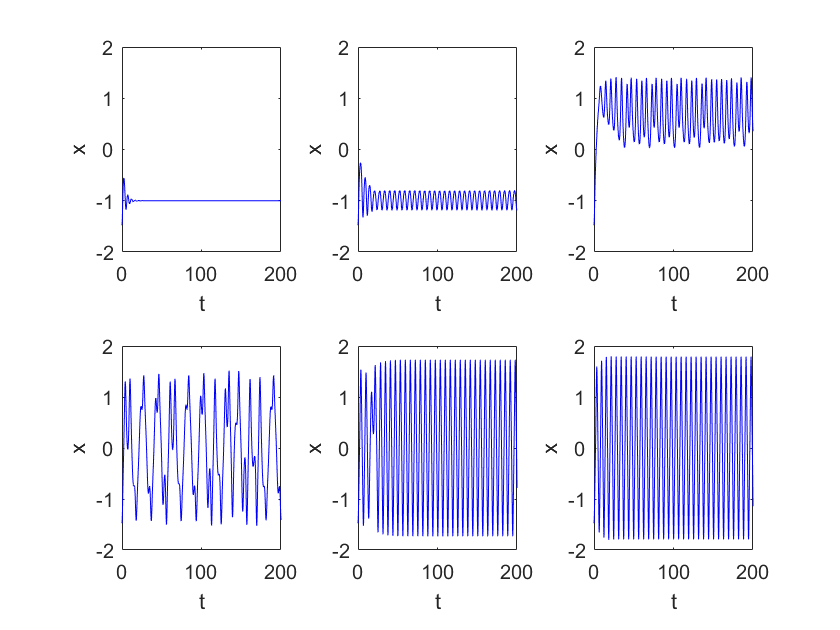
\includegraphics[width=0.7\textwidth]{duffingtime.png}
    \caption{不同周期振幅$A$取值时,Duffing 方程输出时域图}
 \end{figure}

 \begin{figure}[!htbp]
    \centering
    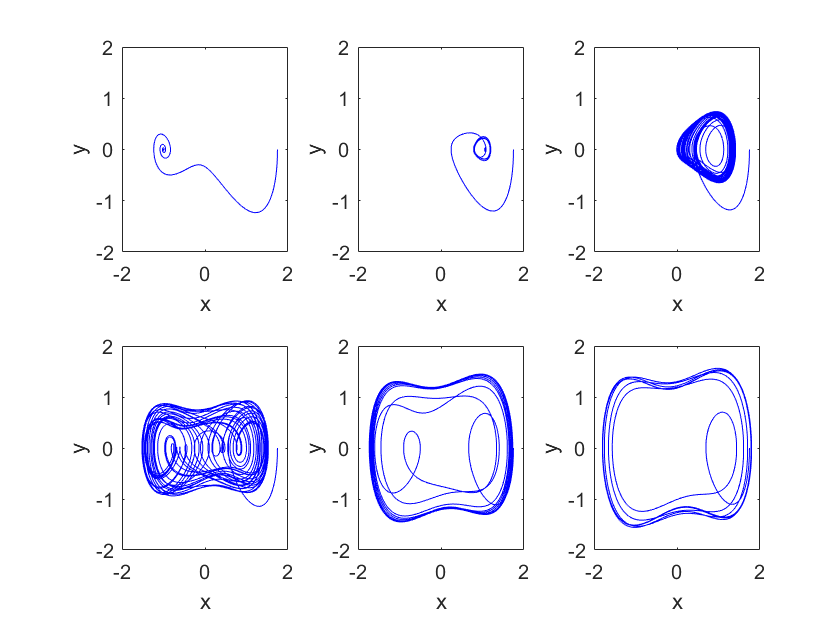
\includegraphics[width=0.7\textwidth]{duffingphase.png}
    \caption{不同周期振幅$A$取值时,Duffing 方程输出相图}
 \end{figure}

所谓分岔是指对于含参数的系统,当参数变动并经过某些临界值时,系统的定态性质
(如平衡状态或者周期运动的数目和稳定性)会发生突然的变化。分岔图则绘制了系统的庞加莱截面输出随参数的变化图,
可用于比较微小参数扰动对系统指标的影响,是系统稳定性的直观衡量。 下图*给出了Duffing 方程输出$x$随周期驱动幅度$A$变化的分岔图(借助庞加莱截面),
也可以看到随着周期驱动幅度$A$的变化,Duffing 方程从吸引子走向混沌、大周期运动的过程。
 \begin{figure}[!htbp]
    \centering
    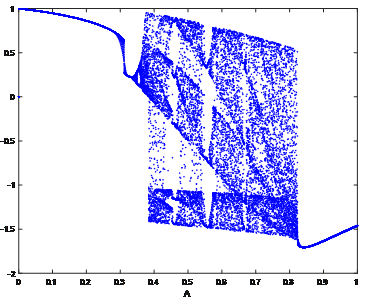
\includegraphics[width=0.5\textwidth]{30.png}\caption{Duffing 方程随周期振幅$A$变化的分岔图}
 \end{figure}


基于上述经典的Holmes型 Duffing 方程(3.1),本文提出如下具有$N$个节点的以WS小世界网络方式进行连接的Duffing复杂网,即Duffing- WS型小世界网络,其动力学方程为:
\begin{equation}
    \ddot{x}_{i}=-\gamma \dot{x}_{i}+a x_{i}-b x_{i}{ }^{3}+\varepsilon \sum_{j=1}^{N} a_{i j}\left(x_{j}-x_{i}\right)+A \sin (\Omega t), i=1,2, \ldots, N
\end{equation}
其中,$x_i(t)$为第$i$个节点的输出状态变量, $i=1,2,\ldots,N$。$A\sin(\Omega t)$为周期驱动力, 
$\varepsilon \sum_{j=1}^{N} a_{i j}\left(x_{j}-x_{i}\right)$表示其它节点对第$i$个节点的耦合作用项, 称为耦合项,$\varepsilon$为网络耦合强度,
$\left(a_{ij}\right)_{N\times N}$为网络的邻接矩阵。一般的,对于一个无权无向的简单连通网络来说,
如果第$i$个节点和第$j$个节点之间有连接,则$a_{ij} = 1$;否则$a_{ij} = 0$。

这里我们采用Watts 和 Strogatz 提出的WS小世界网络作为网络连接拓扑结构[3],其连接方式按如下方式进行:

(1)首先, $N$个节点连接形成一个规则的相邻网络,每个节点与它最近邻的$K$个节点相连,这里$K$称为重连度;
(2)而后以概率$p$ (称为重连概率)随机地重新连接网络中的每条边,
即将边的一个端点保持不变, 而另一个端点取为随机选择的一个节点, 且规定任意两个不同的节点之间至多只能有一条边, 每一个节点都不能有边与自身相连。

对于WS小世界网络而言,当$p = 0$,模型为规则网;当$p = 1$时则为随机网;当$0 < p < 1$,则得到介于规则网与随机网之间的小世界网络。

图*给出了节点数为$N=50$,连接度为$K = 4$,重连概率$p = 0.5$的Duffing-WS型小世界网络的连接拓扑结构图。
\begin{figure}[!htbp]
   \centering
   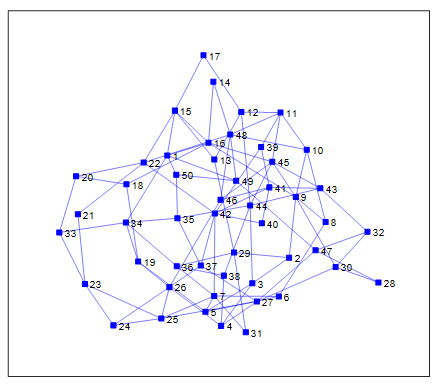
\includegraphics[width=0.6\textwidth]{WStop.png}\caption{Duffing-WS型小世界网络的连接拓扑结构图}
\end{figure}
通过引入Laplacian矩阵为$L=\left(l_{ij}\right)_{N\times N},l_{ij}=\begin{cases}
    -a_{ij},i\neq j \\ \sum_{j\neq i}a_{ij},i=j
\end{cases}$,则方程(3.2)可以改写为如下形式:
\begin{equation}
    \ddot{x}_{i}=-\gamma \dot{x}_{i}+a x_{i}-b x_{i}^{3}+A \sin (\Omega t)-\varepsilon\sum_{j=1}^{N} l_{i j} x_{j}
\end{equation}
由Laplacian矩阵的性质可知,$L$是一个实对称的弱对角占优矩阵,且对角元均非负,所以是半正定的。
事实上,复杂网络的邻接矩阵或Laplacian矩阵全面地刻画了网络节点之问的相互关系,其特征值和特征向量则揭示了网络拓扑及其整体行为的信息。

\section{Duffing-WS型小世界网络基本动力学特性研究}
\subsection{分岔图分析}
我们的研究发现,当驱动力幅度A值在(0,1)范围变化时,随着A值的变化,Duffing-WS小世界网络的各个粒子输出也将呈现小尺度周期运动、
我们的研究发现,当驱动力幅度$A$值在(0,1)范围变化时,随着$A$值的变化,Duffing-WS小世界复杂网络(*)的各个节点输出也将呈现小尺度周期运动、
倍周期分岔、混沌和大尺度周期运动等状态。我们首先借助庞加莱截面给出Duffing-WS小世界网络的分岔图。 分岔图绘制了系统的庞加莱截面输出随参数的变化图,可用于比较微小参数扰动对系统指标的影响,
在本文中用来衡量混沌现象。

取庞加莱截面为$t=j T, T=2 \pi / \Omega$,在此截面上引入如下宏观变量$\sigma(j T)$来描述系统的集体行为:
\begin{equation}
    \sigma(j T)=\frac{1}{N} \sum_{i=1}^N x_i(j T)
\end{equation}
图(a)中给出了借助庞加莱截面单个 Duffing 方程的解随驱动力幅度 $A$ 变化的分岔图。图 (b) 给出了借助 $\sigma(j T)$, 
节点个数为 $N=100$ 的 Duffing-WS 型 小世界网络关于幅度 $A$ 的变化的分岔图。和图 1 中单个 Duffing 方程关于幅度 $A$ 
的分岔图对比可知, Duffing-WS 型小世界网络的分岔图事实上也历经了小尺度 周期运动、倍周期分岔、混沌和大尺度周期运动等状态,
 在大尺度周期状态之 后又进入了短暂的混沌状态, 因此其分岔图具有更为复杂的特性。
 \begin{figure}[!htbp]
    \centering
    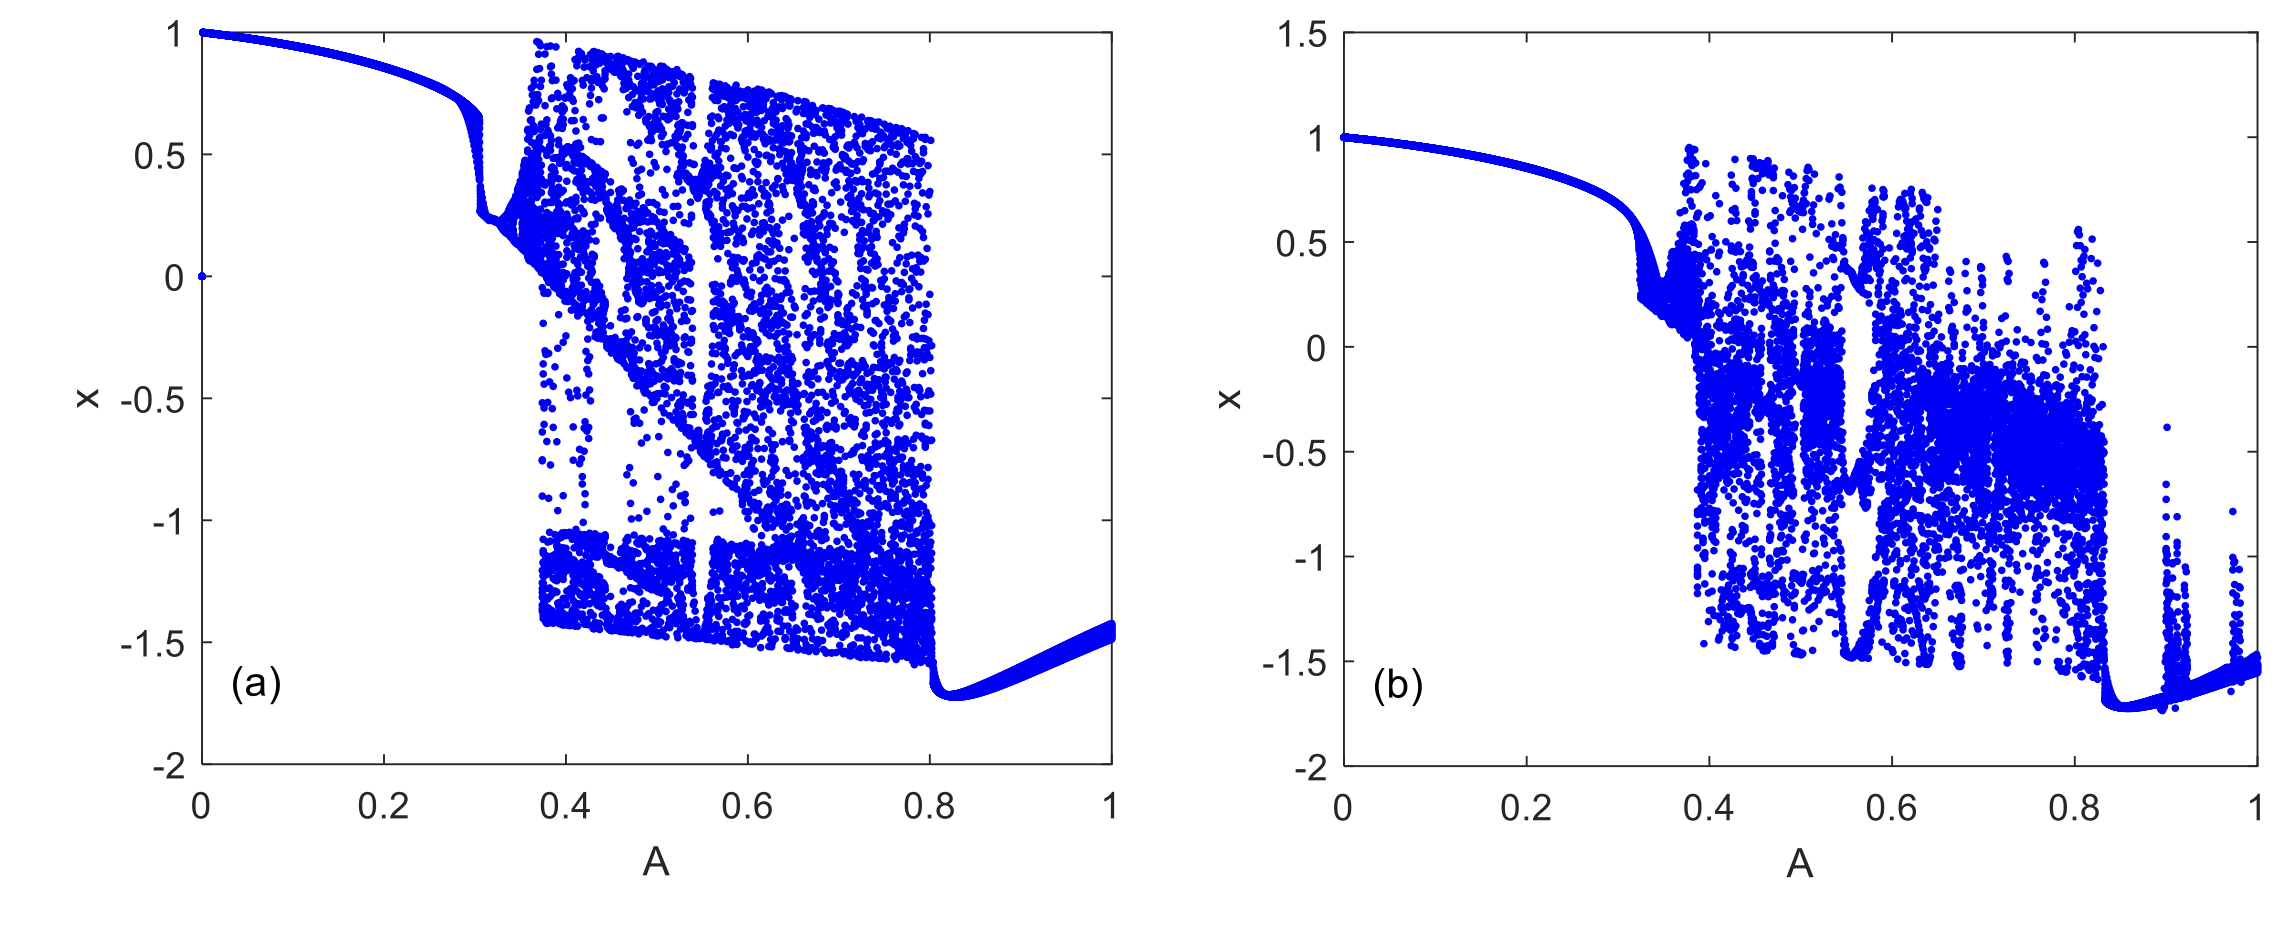
\includegraphics[width=0.8\textwidth]{31.png}
    \caption{分叉图演示}
 \end{figure}
\subsection{基于LE指数的混沌动力学分析}
从3.1节可以看出,通过分岔图并不容易定量分析复杂系统的混沌行为,而对耦合系统混沌进行分析的另外一个指标为系统的
LE指数。LE指数是衡量系统动力学特性的一个重要定量指标,表现了系统在相空间中相邻轨道间收缩或发散的平均指数率。

这一节我们利用变分法推导 Duffing-WS 型小世界网络的最大 LE 指数表 达式, 利用最大 LE 指数来研究其混沌现象,
并分析小世界网络重连度 $K$, 重连 概率 $p$ 和耦合强度 $\varepsilon$ 等对复杂系统处于混沌运动状态参数范围的影响。
其中,LE指数采用数值模拟的方式给出,其计算方法的理论依据已在第二章给出。
通过令
\begin{eqnarray*}
z_i=\Omega t,\left. z_i\right|_{t=0}=0
\end{eqnarray*}
可将Duffing-WS 型小世界网络模型(*)的非自治方程变成如下的自治方程组:
 \begin{equation}
    \left\{\begin{array}{l}
    \dot{x}_i=y_i \\
    \dot{y}_i=-\gamma y_i+a x_i-b x_i^3+A \sin \left(z_i\right)-\varepsilon \sum_{j=1}^N l_{i j} x_j \\
    \dot{z}_i=\Omega
    \end{array}\right.
\end{equation}
假设 $s(t)$ 是单个 Duffing 方程(1)的解, 引入变分:
\begin{equation}
    \delta_{x i}=x_i(t)-s(t), \delta_{y i}=y_i(t)-\dot{s}(t),
\end{equation}
并结合自治方程组(*)可得到 Duffing-WS 小世界网络的变分方程为:
\begin{equation}
    \left\{\begin{array}{l}
    \dot{\delta}_{x i}=\delta_{y i} \\
    \dot{\delta}_{y i}=-\gamma \delta_{y i}+a \delta_{x i}-3 b x_i^2 \delta_{x i}+A \cos \left(z_i\right) \delta_{z i}-\varepsilon \sum_{j=1}^N l_{i j} \delta_{x j} \\
    \dot{\delta}_{z i}=0
    \end{array}\right.
\end{equation}
在不失去普遍性的情况下, 在上述变分方程中令集合 $\delta_{z i}=0$, 则变分方程可以简化为:
\begin{equation}
    \left\{\begin{array}{l}
    \dot{\delta}_{x i}=\delta_{y i} \\
    \dot{\delta}_{y i}=-\gamma \delta_{y i}+a \delta_{x i}-3 b x_i^2 \delta_{x i}-\varepsilon \sum_{j=1}^N l_{i j} \delta_{x j}
    \end{array}\right.
\end{equation}
则根据定义,本章所提Duffing-WS型小世界网络的最大LE指数表达式为:
\begin{equation}
    \lambda_{\max }=\lim _{T \rightarrow \infty} \frac{\log \left(\sqrt{\sum_{i=1}^N\left|\delta_{x i}(T)\right|+\left|\delta_{y i}(T)\right|}\right)}{T}
\end{equation}
在下面的章节中,我们利用上式计算不同参数情况下的Duffing- WS型小世界网络平均最大LE指数关于周期幅度变化的曲线,
其中LE指数大于0的区域被视为系统处于混沌运动的区域。网络的粒子个数固定为$N=100$,每条曲线均是对50个样本轨道平均后所得。
Duffing方程中的参数固定为$a=1,b=1,\gamma=0.5,\Omega=1$。此外,本文Duffing- WS型小世界网络(*)及其对于变分方程组(*)
的数值模拟均基于我们在第*节给出的微分方程四阶龙格库塔算法。
\subsection{耦合强度对混沌的影响}
图(a)-(c)给出了不同的耦合强度 $\varepsilon$ 下平均最大 LE 指数随幅度 $A$ 变化的曲线, 重连概率均为 $p=0.5$ 。
在图(a)中 $K=2$, 当耦合强度 $\varepsilon$ 较小时 (如 $\varepsilon=0,0.2,0.4)$, 随着 $\varepsilon$ 的增大,
LE 指数大于 0 的混沌区域扩大; 当耦合强度 $\varepsilon$ 较大时 (如 $\varepsilon=$ $0.6,0.8,1,2)$, 
随着 $\varepsilon$ 的增加, LE 指数大于 0 的混沌区域则逐渐收缩, 混沌受到抑制。在这种情况下, 
由于重连度非常小节点之间的连接程度不够, 小的耦合强 度的增强反而增强系统的混沌运动; 而只有耦合强度大到一定程度, 
更大的耦合强度使得系统协同性增强, 才能抑制系统的混沌运动。\par
在图(b)中 $K=20$, 可以看到, 当 $\varepsilon=0$ 时, 小世界网络退化成独立的 $N$ 个 Duffing系统, 此时混沌区域最大, 
而当 $\varepsilon>0$ 时, 小世界网络各个节点之间存在 耦合作用, 网络的混沌区域收缩; 而此时由于重连度 $K$ 值较大, 平均 LE 指数随
幅度 $A$ 变化的曲线在不同的耦合强度 $\varepsilon$ 下基本一致, 也就是说此时小世界网络的混沌运动区域对耦合强度 
$\varepsilon$ 具有鲁棒性。同样, 在图(c)中 $K=48$, 可以看到, 随着 $\varepsilon$ 增加, 混沌区域的变化同样不明显。
综上可以看到, 和传统的规则网络不同, 本文所提 Duffing-WS 型小世界网络的耦合强度 $\varepsilon$ 
对混沌区域的影响并不是线性的, 当重连度 $K$ 较小时, 随着耦合强度的增加混沌区域呈现出先扩大后缩小的变化, 
$K$ 较大时 $\varepsilon$ 的增强对混沌区域影响不明显。\par
\begin{figure}[!htbp]
    \centering
    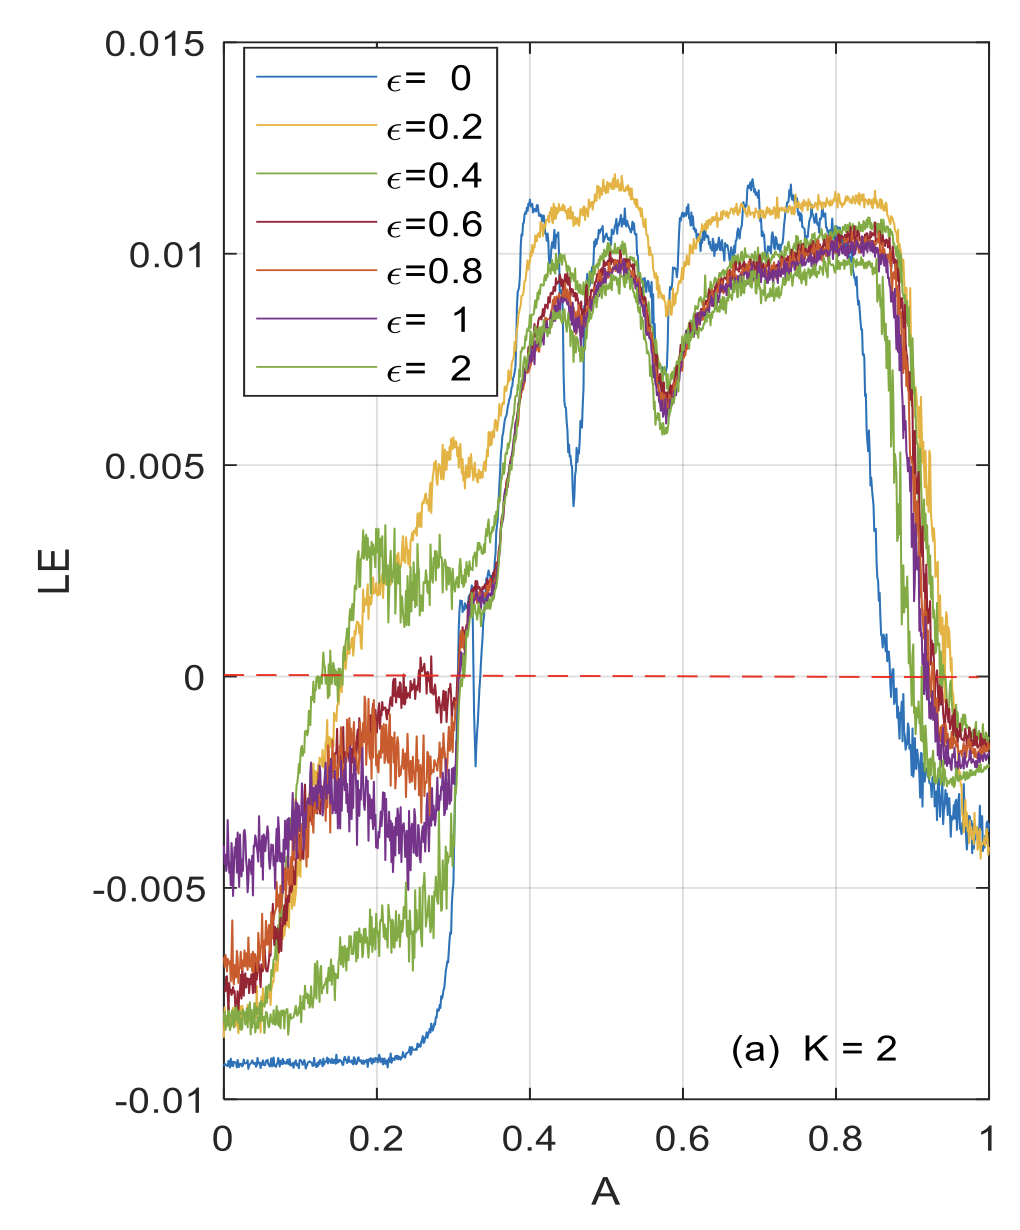
\includegraphics[width=0.48\textwidth]{k2.png}
    \caption{$K=2$时耦合强度对混沌的影响}
\end{figure}
在图(a)中 $K=2$, 当耦合强度 $\varepsilon$ 较小时 (如 $\varepsilon=0,0.2,0.4)$, 随着 $\varepsilon$ 的增大,
LE 指数大于 0 的混沌区域扩大; 当耦合强度 $\varepsilon$ 较大时 (如 $\varepsilon=$ $0.6,0.8,1,2)$,
随着 $\varepsilon$ 的增加, LE 指数大于 0 的混沌区域则逐渐收缩, 混沌受到抑制。在这种情况下,
由于重连度非常小节点之间的连接程度不够, 小的耦合强 度的增强反而增强系统的混沌运动; 而只有耦合强度大到一定程度,
更大的耦合强度使得系统协同性增强, 才能抑制系统的混沌运动。\par
\begin{figure}[!htbp]
    \centering
    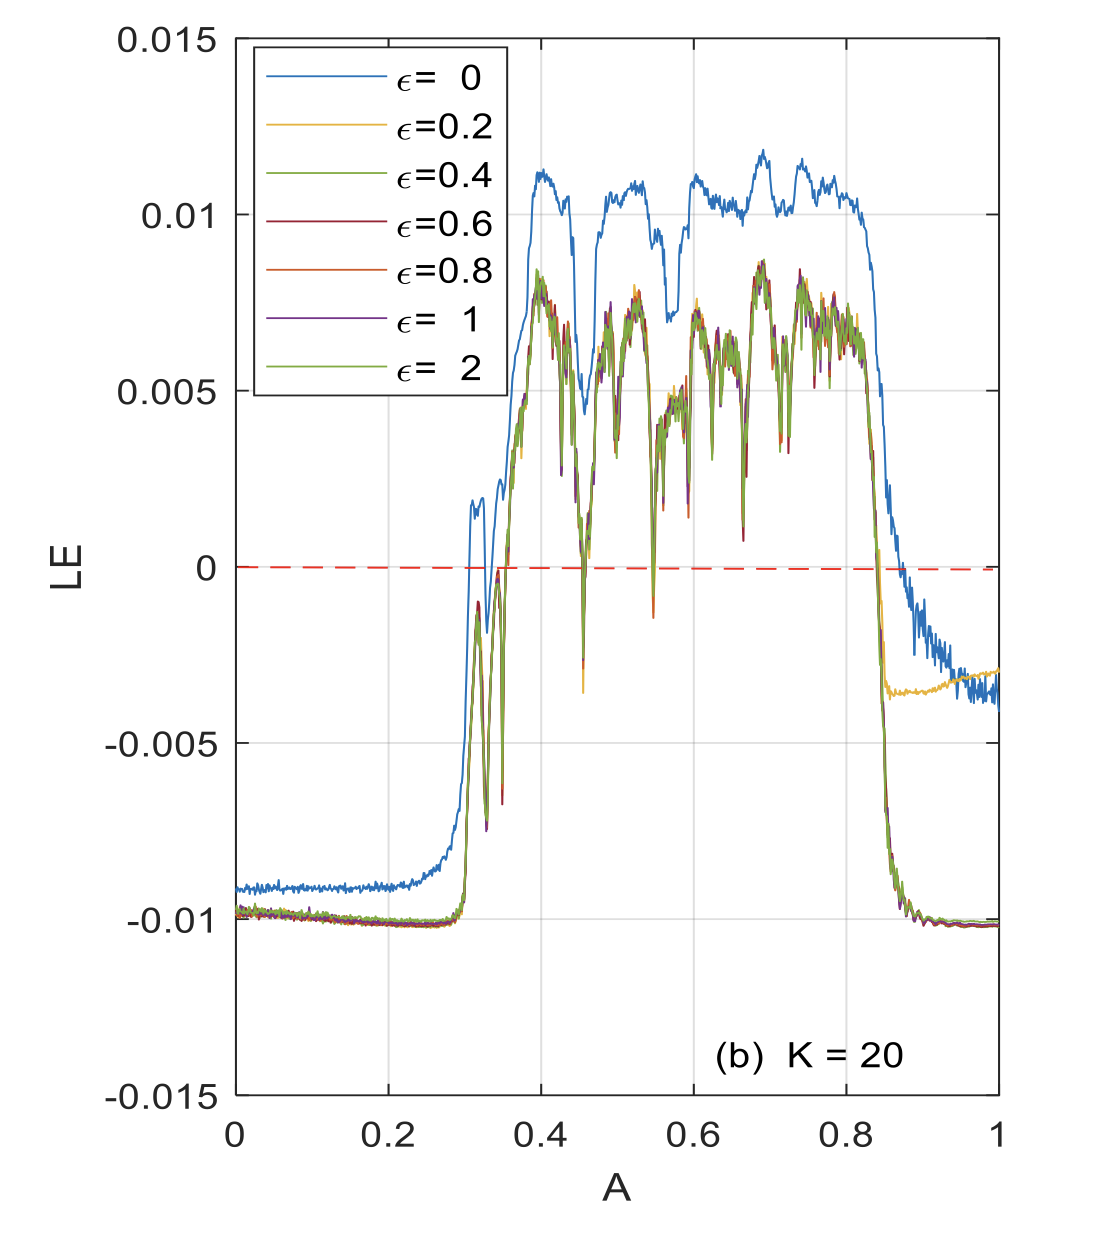
\includegraphics[width=0.5\textwidth]{k20.png}
    \caption{$K=20$时耦合强度对混沌的影响}
\end{figure}

在图(b)中 $K=20$, 可以看到, 当 $\varepsilon=0$ 时, 小世界网络退化成独立的 $N$ 个 Duffing系统, 此时混沌区域最大,
而当 $\varepsilon>0$ 时, 小世界网络各个节点之间存在 耦合作用, 网络的混沌区域收缩; 而此时由于重连度 $K$ 值较大, 平均 LE 指数随
幅度 $A$ 变化的曲线在不同的耦合强度 $\varepsilon$ 下基本一致, 也就是说此时小世界网络的混沌运动区域对耦合强度
$\varepsilon$ 具有鲁棒性。\par
\begin{figure}[!htbp]
    \centering
    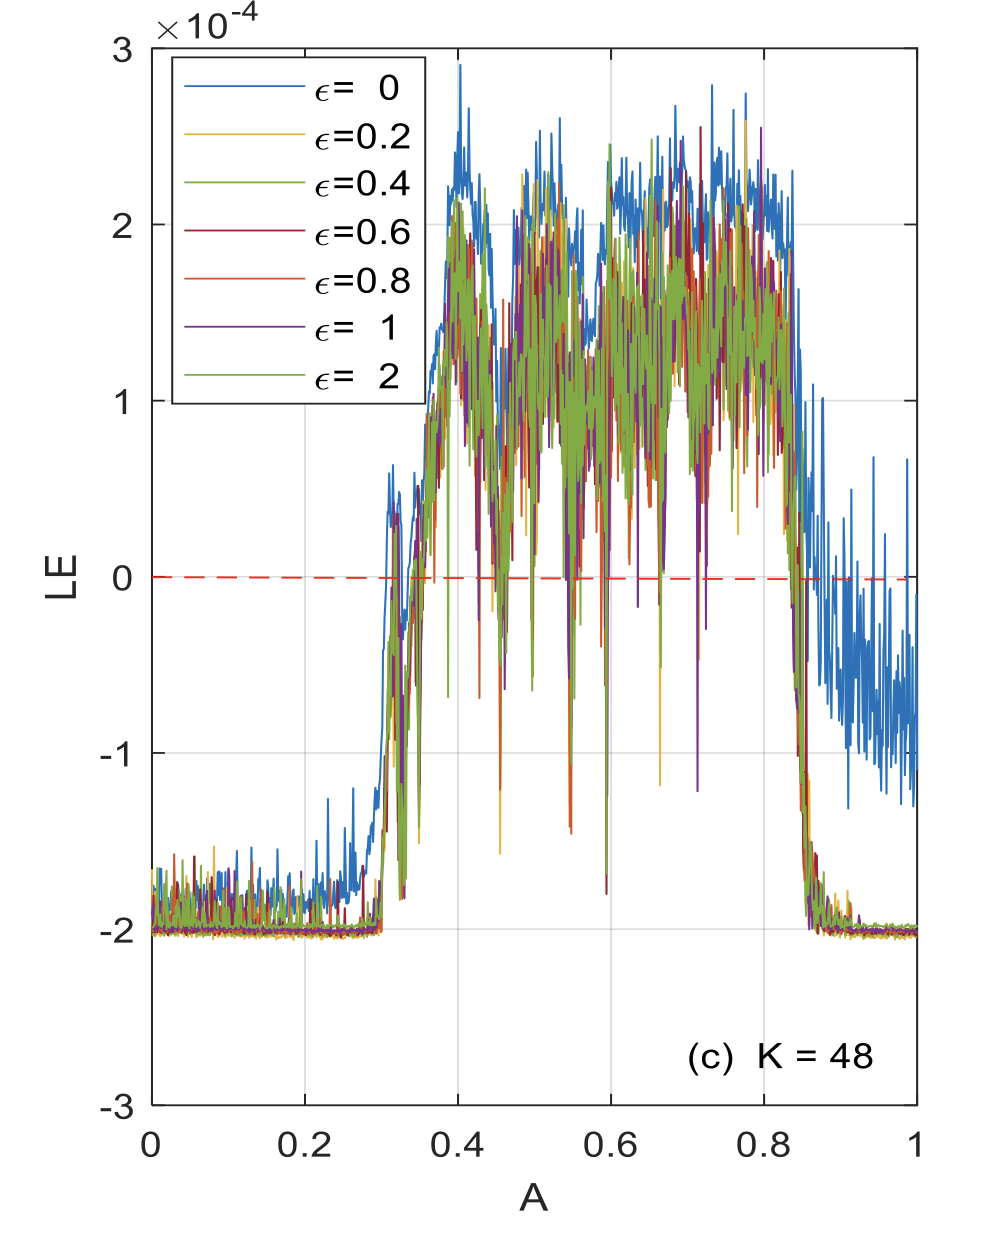
\includegraphics[width=0.45\textwidth]{k48.png}
    \caption{$K=48$时耦合强度对混沌的影响}
\end{figure}
同样, 在图(c)中 $K=48$, 可以看到, 随着 $\varepsilon$ 增加, 混沌区域的变化同样不明显。
综上可以看到, 和传统的规则网络不同, 本文所提 Duffing-WS 型小世界网络的耦合强度 $\varepsilon$
对混沌区域的影响并不是线性的, 当重连度 $K$ 较小时, 随着耦合强度的增加混沌区域呈现出先扩大后缩小的变化,
$K$ 较大时 $\varepsilon$ 的增强对混沌区域影响不明显。


\subsection*{重连度$K$对混沌的影响}
我们接着分析重连度$K$对Duffing- WS型小世界网络混沌现象的影响。图(a)-(c)给出了不同的重连度 $K$ 下平均 LE 指数随幅度 $A$ 变化的曲线, 耦合强度均为 $\varepsilon=0.5$ 。\par
\begin{figure}[!htbp]
    \centering
    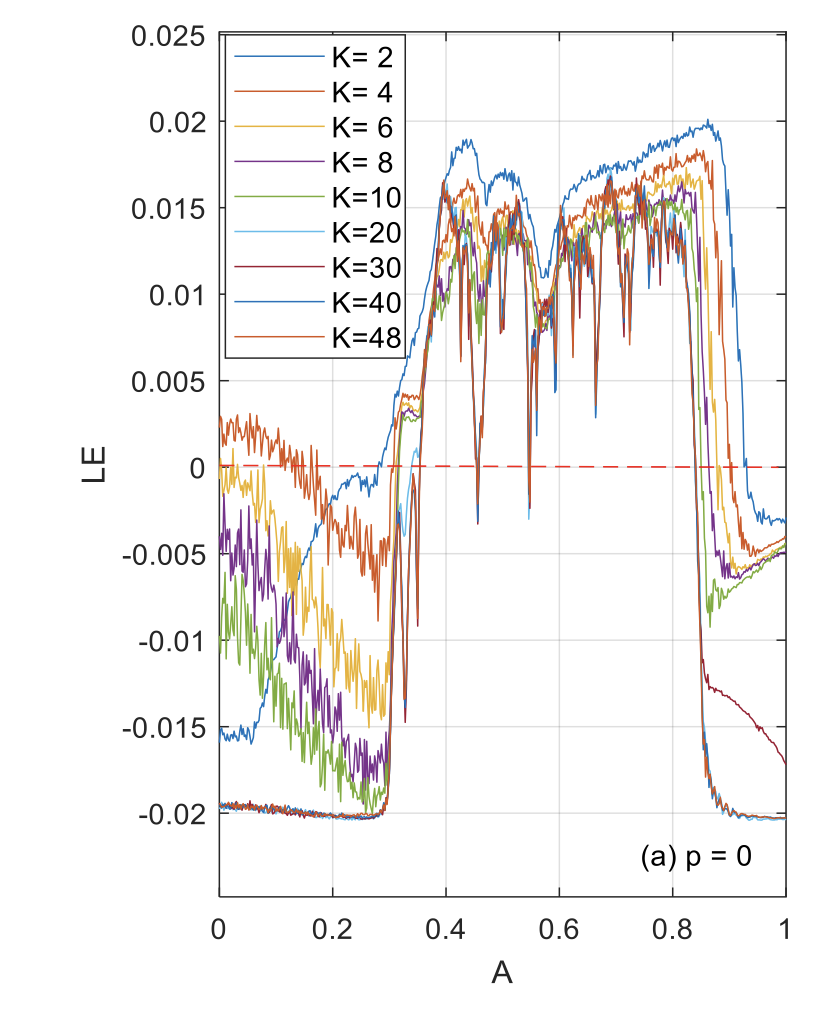
\includegraphics[width=0.5\textwidth]{pa.png}
    \caption{$p=0$时连接度对混沌的影响}
\end{figure}
可以看出, 在图(a)中 $p=0$, 耦合网络为规则的最近邻耦合 网络, 当重连度 $K$ 较小时 $(K=2,4,6,8,10)$,
随着重连度 $K$ 的增加, LE 指数大于 0 的混沌区域先扩大再收缩, 当 $K=4$ 时混沌区域达到最大; 随后,
随着重连度 $K$ 增加到一定程度以后 $(K=20,30,40,48)$, 混沌区域随着 $K$ 值的增加而有略微地缩小,
但总体上差异不大。这说明对于规则网络, 只有足够大的重连度才会抑制 系统混沌, 较小的重连度反而增加系统的混沌运动。\par
\begin{figure}[!htbp]
    \centering
    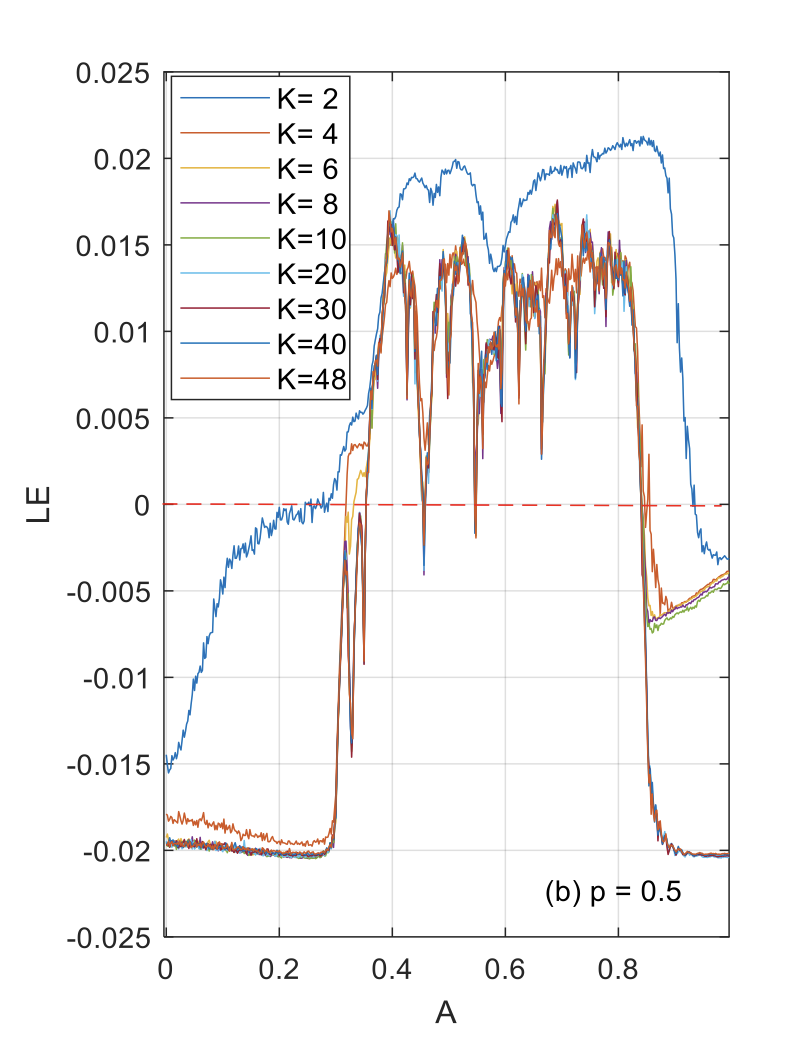
\includegraphics[width=0.45\textwidth]{pb.png}
    \caption{$p=0.5$时连接度对混沌的影响}
\end{figure}
在图(b)中 $p=0.5$, 此时网络为标准的小世界模型。 $K=2$ 与$K$ 值 LE 曲线 有显著不同, 所对应的混沌区域最大,
LE 指数在各个振幅处的值都最高, 可见 重连度 $K$ 较低时更容易产生较大的混沌范围。 $K=4,6$ 比起 $K=2$ 的 LE 曲线, 其
大于 0 的区域明显缩小, 即重连度的增加明显抑制了网络混沌运动; 随着 $K$ 值进 一步增加, 系统 LE 曲线几乎没有变化,
这是因为当重连度足够高时, 系统各节 点输出间差异很小, 混沌区域几乎一致。\par
\begin{figure}[!htbp]
    \centering
    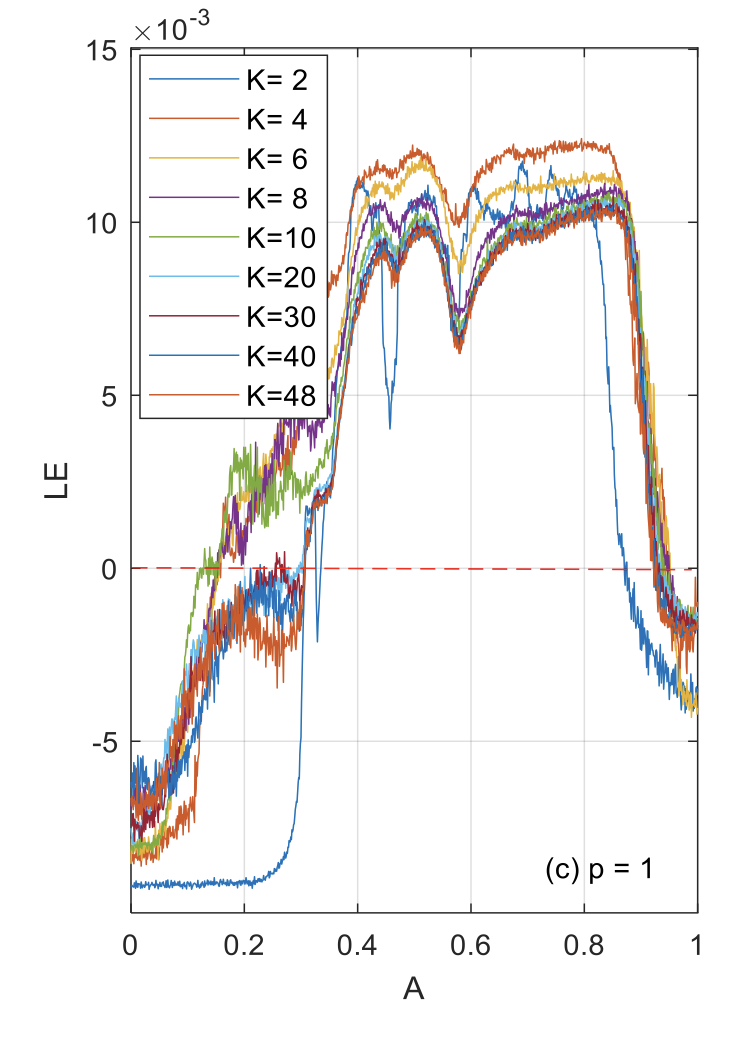
\includegraphics[width=0.43\textwidth]{pc.png}
    \caption{$p=1$时连接度对混沌的影响}
\end{figure}
在图 (c)中 $p=1$, 此时网络为完全的随机网络。可以看出, $K$ 足够大时 LE 曲线的一致性会被打破,
重连度对混沌区域的控制不再呈现明显的规律。当 $K=2$ 时混沌区域反而最小, 而中间大小的重连度 $(K=4,6,8,10)$ 混沌区域却最大。
同时, 对比完全规则网络 $(p=0)$ 与小世界网络 $(p=0.5)$, 完全随机网络的混 沌区域更大且 LE 指数更低。
\subsection*{重连概率$p$对混沌的影响}
最后我们分析重连概率$p$对Duffing- WS型小世界网络混沌现象的影响。图(a)-(c)给出了不同的重连概率
 $p$ 下平均LE指数随幅度 $A$ 变化的曲线, 耦 合强度均为 $\varepsilon=0.5$。
图(a)-(c)给出了不同的重连概率 $p$ 下平均LE指数随幅度 $A$ 变化的曲线, 耦 合强度均为 $\varepsilon=0.5$ 。
在图 (a)中 $K=2$, 在图(b)中 $K=20$, 可以看出, 不同重 连概率 $p$ 对混沌区域的影响不明显, 
差异主要体现在 LE 指数的高低上, 重连概 率 $p$ 越大, LE 指数值越小。在图中 $K=48$, 在这种情形下混沌区域明显后
移。总的来说,此时小世界网络的混沌区域对重连概率$p$具有鲁棒性。
\begin{figure}[!htbp]
    \centering
    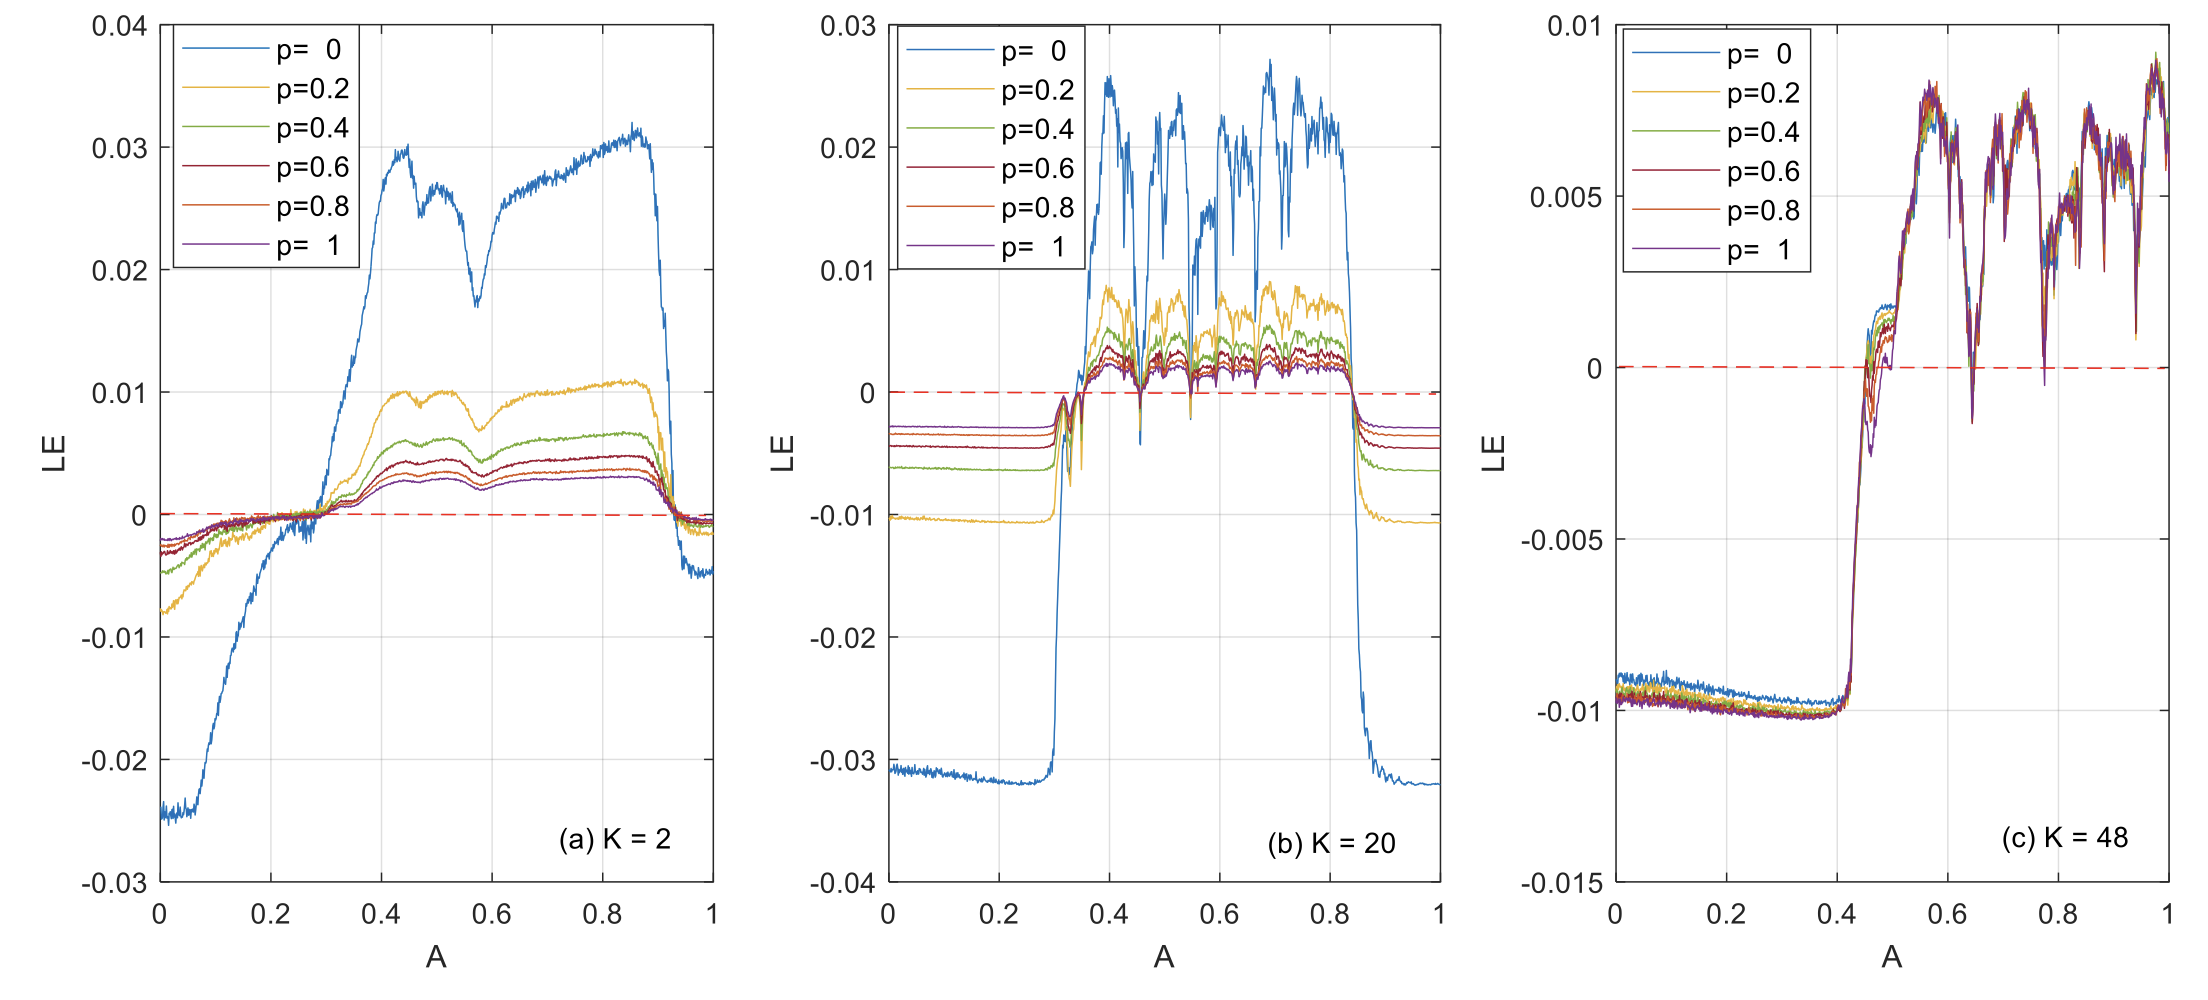
\includegraphics[width=\textwidth]{34.png}
    \caption{重连概率对混沌的影响}
\end{figure}
\subsection{同步性分析}
事实上,大量耦合粒子的同步化问题最早由1998年给出的基于变分方程的主稳定函数方法而得到妥善地解决[*]。下面我们仍然基于变分法给出本章所提Duffing-WS小世界网络(*)的主稳定函数,并由此分析Duffing-WS小世界网络的同步性。
Duffing-WS小世界网络的变分方程已由(*)式给出,令
\begin{eqnarray*}
\boldsymbol{\delta}_{i}=\left[\delta_{xi}, \delta_{yi}, \delta_{zi}\right]^T,
\end{eqnarray*}
则Duffing-WS 小世界网络的变分方程(*)可以简化为如下的矢量形式:
\begin{equation}
    \dot{\boldsymbol{\delta}}_i=D f(\mathbf{S}) \boldsymbol{\delta}_i-c \sum_{j=1}^N l_{i j} H \boldsymbol{\delta}_j, i=1,2, \ldots, N
\end{equation}
其对应的孤立节点动力学函数为
\begin{eqnarray*}
 f(\mathbf{X})=\left[\begin{array}{c}y \\ -\gamma y+a x-b x^3+A \sin (z) \\ \Omega\end{array}\right],
\end{eqnarray*}
节点内连矩阵为:
\begin{eqnarray*}
H=\left[\begin{array}{lll}
0 & 0 & 0 \\
1 & 0 & 0 \\
0 & 0 & 0
\end{array}\right].
\end{eqnarray*}

令同步流形为 $\mathbf{S}(t)=(s(t), \dot{s}(t), \Omega t)^T$, 即孤立节点动力学方程 $\dot{\mathbf{S}}(t)=f(\mathbf{S})$ 的解。
$D f(\mathbf{S})$ 则为单节点动力学函数在同步流形 $\mathbf{S}(t)=(s(t), \dot{s}(t), \Omega t)^T$ 处的雅可比矩阵, 有
\begin{equation}
    D f(\mathbf{S})=\left[\begin{array}{ccc}
    0 & 1 & 0 \\
    a-3 b s^2(t) & -\gamma & A \cos (\Omega t) \\
    0 & 0 & 0
    \end{array}\right]
\end{equation}
令 $\boldsymbol{\delta}=\left(\boldsymbol{\delta}_1, \ldots, \boldsymbol{\delta}_N\right)$, 则(3.11)式可以改写为
\begin{equation}
    \dot{\boldsymbol{\delta}}=D f(\mathbf{S}) \boldsymbol{\delta}-c H \boldsymbol{\delta} L^T
\end{equation}
不妨假设Laplacian矩阵可对角化 (即为无向图情况)), $L^T=P \Lambda P^{-1}, \Lambda=\operatorname{diag}\left(\lambda_1, \ldots, \lambda_N\right)$, 
令 $\boldsymbol{\eta}=\boldsymbol{\delta} P$, 则方程组又等价于如下的方程组:
\begin{equation}
    \begin{gathered}
    \dot{\boldsymbol{\eta}}_1=D f(\mathbf{S}) \boldsymbol{\eta}_1, k=1,2, \ldots, N \\
    \dot{\boldsymbol{\eta}}_k=\left[D f(\mathbf{S})-c \lambda_k H\right] \boldsymbol{\eta}_k, k=2, \ldots, N
    \end{gathered}
\end{equation}
第一式对应于与同步流形平行方向的扰动,为保证同步流形的稳定性,需要第二式描述的$N-1$个子系统是渐近稳定的。注意到除非$s(t)$是平衡点,
否则第二式中的每个子系统都是时变系统,判断同步流形稳定的一个常用判据是要求主稳定方程的所有Lyapunov指数全为负值。
方程组(*)所对应的主稳定方程可以写为:
\begin{equation}
    \dot{\boldsymbol{y}}=\boldsymbol{M}(\alpha)\boldsymbol{y}
\end{equation}
其中 $\boldsymbol{M}(\alpha)=\left[\begin{array}{ccc}0 & 1 & 0 \\ a-3 b s^2(t)-\alpha & -\gamma & A \cos (\Omega t)
\\ 0 & 0 & 0\end{array}\right], \alpha=c \lambda_k$。这里假设主稳定方程的最大李亚普洛夫指数为 $LE(\alpha)$。

将主稳定方程和单个节点的Duffing方程联立,得到
\begin{equation}
    \left\{\begin{array}{l}
    \dot{s}_1=s_2 \\
    \dot{s}_2=-\gamma s_2+a s_1-b s_1^3+A \sin (\Omega t) \\
    \dot{y}_1=y_2 \\
    \dot{y}_2=\left(a-3 b s_1^2-\alpha\right) y_1-\gamma y_2+A \sin (\Omega t) y_3 \\
    \dot{y}_3=0
    \end{array}\right.
\end{equation}
于是,其最大 Lyapunov 指数由下式给出:
\begin{equation}
L E(\alpha)=\lim _{T \rightarrow+\infty}
\frac{\ln \left(\left|y_1(T)\right|+\left|y_2(T)\right|\right)}{T}
\end{equation}

下面的图绘制了当周期驱动幅度$A$在[0,1]范围内时,主稳定方程(*)平面Lyapunov指数的相图,即其最大 Lyapunov指数关于参数$\alpha$和振幅$A$的变化图,
其中黑色区域为最大Lyapunov指数非负即不同步的区域。同样,我们按照不同初始值取了50次平均得到最后的结果。\par
\begin{figure}[!htbp]
    \centering
    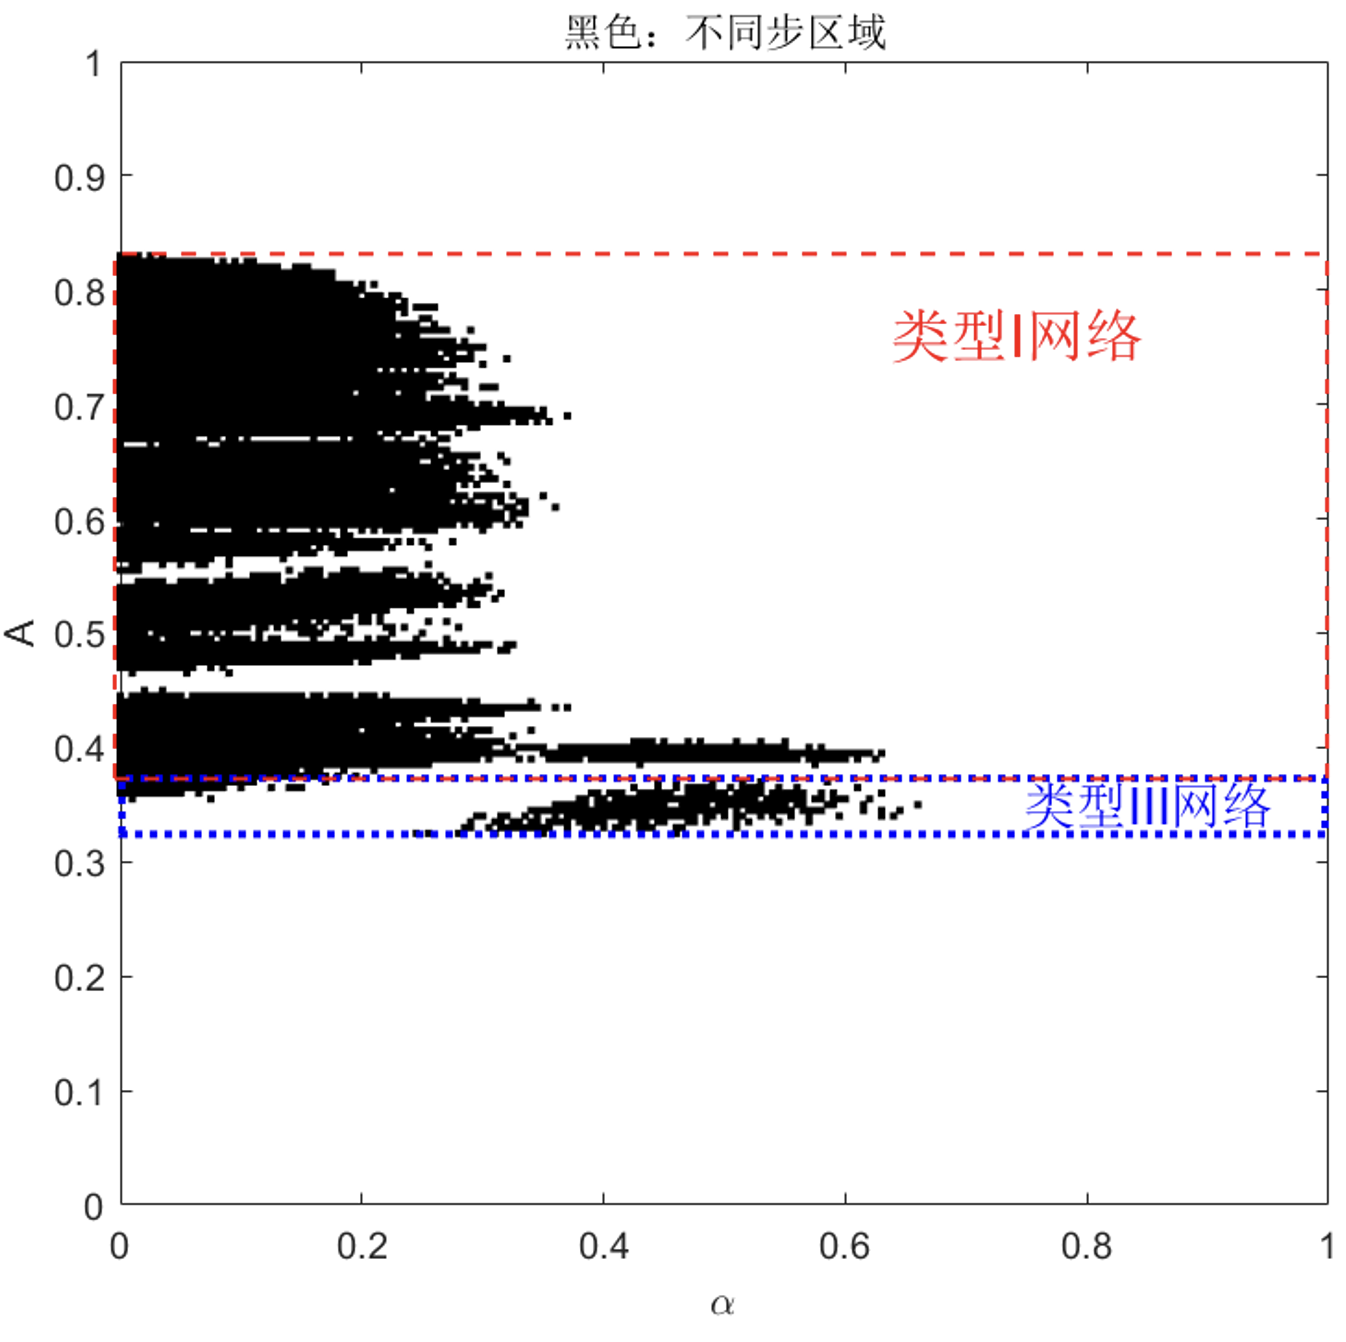
\includegraphics[width=0.6\textwidth]{tb1.png}
    \caption{不同类型网络混沌的振幅范围}
\end{figure}
分析图(*),我们可以得出如下结论:

(1)当 $A \in[0,0.32] \cup[0.83,1]$ 时, 主稳定方程的最大 $\mathrm{LE}$ 指数全为负数, 即我们考虑的Duffing-WS小世界网络(*)的同步化区域为全区域 $S R=(0,+\infty)$,
这时候的系统总是可以达到完全同步 (和耦合网络结构小世界特性无关);\par

(2)当 $A \in[0.33,0.37]$ 时, 网络属于类型$\mathrm{III}$的网络, 其同步化区域为不连通的多区域 $S R=\left(0, \alpha_1\right) \cup\left(\alpha_2,+\infty\right)$,
这时候系统要达到完全同步, 必须满足 $c \lambda_k \in S R, k=2,3, \ldots, N$,
而要同时调整耦合强度和所有特征值全部落入不连通的同步化区域 SR。此时,
如果满足 $c \lambda_2>\alpha_2$, 则 $\alpha_2<c \lambda_2 \leq \ldots \leq c \lambda_N$ 时,
都有 $L E(\alpha)<0$, 同步流形总是稳定的, 系统总能同步。

在这种情况下, 网络Laplacian 矩阵的第二大特征值
$\lambda_2$ 的大小可以作为衡量网络同步化能力的指标, $\lambda_2$ 越 大则系统越容易达到同步, 也就是系统的同步化能力越强。
如果 $\alpha_1<c \lambda_2<\alpha_2$, 则同步流形不稳定, 系统不能同步。如果 $c \lambda_2<\alpha_1$,
则要求 $c \lambda_N<\alpha_1\left(\lambda_N / \lambda_2<c\right)$ 或者 $\alpha_2<c \lambda_3$, 则同步流形稳定,
此时系统同步相对于前 面两种情况更不容易实现。

(3)当 $A \in[0.38,0.82]$ 时, 网络属于类型 $\mathrm{I}$ 的网络, 其同步化区域为无界区域 $S R=\left(\alpha_3,+\infty\right)$,
即当 $\alpha_3<c \lambda_2 \leq \ldots \leq c \lambda_N$ 时, 都有 $L E(\alpha)<0$, 即 $c \lambda_2>\alpha_3$,
同步流形总是稳定的, 系统总能同步。在这种情况下, Laplacian 矩阵的第二大 特征值 $\lambda_2$ 的大小也是可以作为衡量网络同步化能力的指标。\par

综上可知, 对于不同的 $A$ 值, 当 Laplacian 矩阵的第二大特征值 $\lambda_2$ 和耦合系数的乘积 $c \lambda_2$ 充分大时,
系统总能实现同步; 给定耦合系数 $\mathrm{c}$, Laplacian 矩阵 的第二大特征值 $\lambda_2$ 决定了系统的同步能力,
当 $\lambda_2$ 的值较小时, 系统则很有可能 不能同步。但是当增加耦合系数 $\mathrm{c}$ 大于某个值时, 对于系统也总能实现同步。

下图给出了粒子个数为 $\mathrm{N}=20,100$ 时, Duffing-WS小世界网络 Laplacian 矩阵的第二大特征值 $\lambda_2$在不同的 $\mathrm{K}$ 值下随重连概率 $\mathrm{p}$
变化的曲线(平均 100次)。可以看到当连接度较小 $(\mathrm{K}=1)$时, 第二大特征值 $\lambda_2$ 随着重连概率增加先减小后增加,
说明此时较小或较大的重连概率均有利于增加系 统同步; 随着连接度增加(左图, $K=2,3,4,5,6$ ), 第二大特征值 $\lambda_2$
随着重连概率增加先增加后减小, 说明此时适当大小的重连概率有利于增加系统的同步; 当连接 度继续增加而接近 $\mathrm{N} / 2$ 时,
第二大特征值 $\lambda_2$ 随着重连概率增加而减小, 说明较小的重连概率有利于增加系统的同步。\par
\begin{figure}[!htbp]
    \centering
    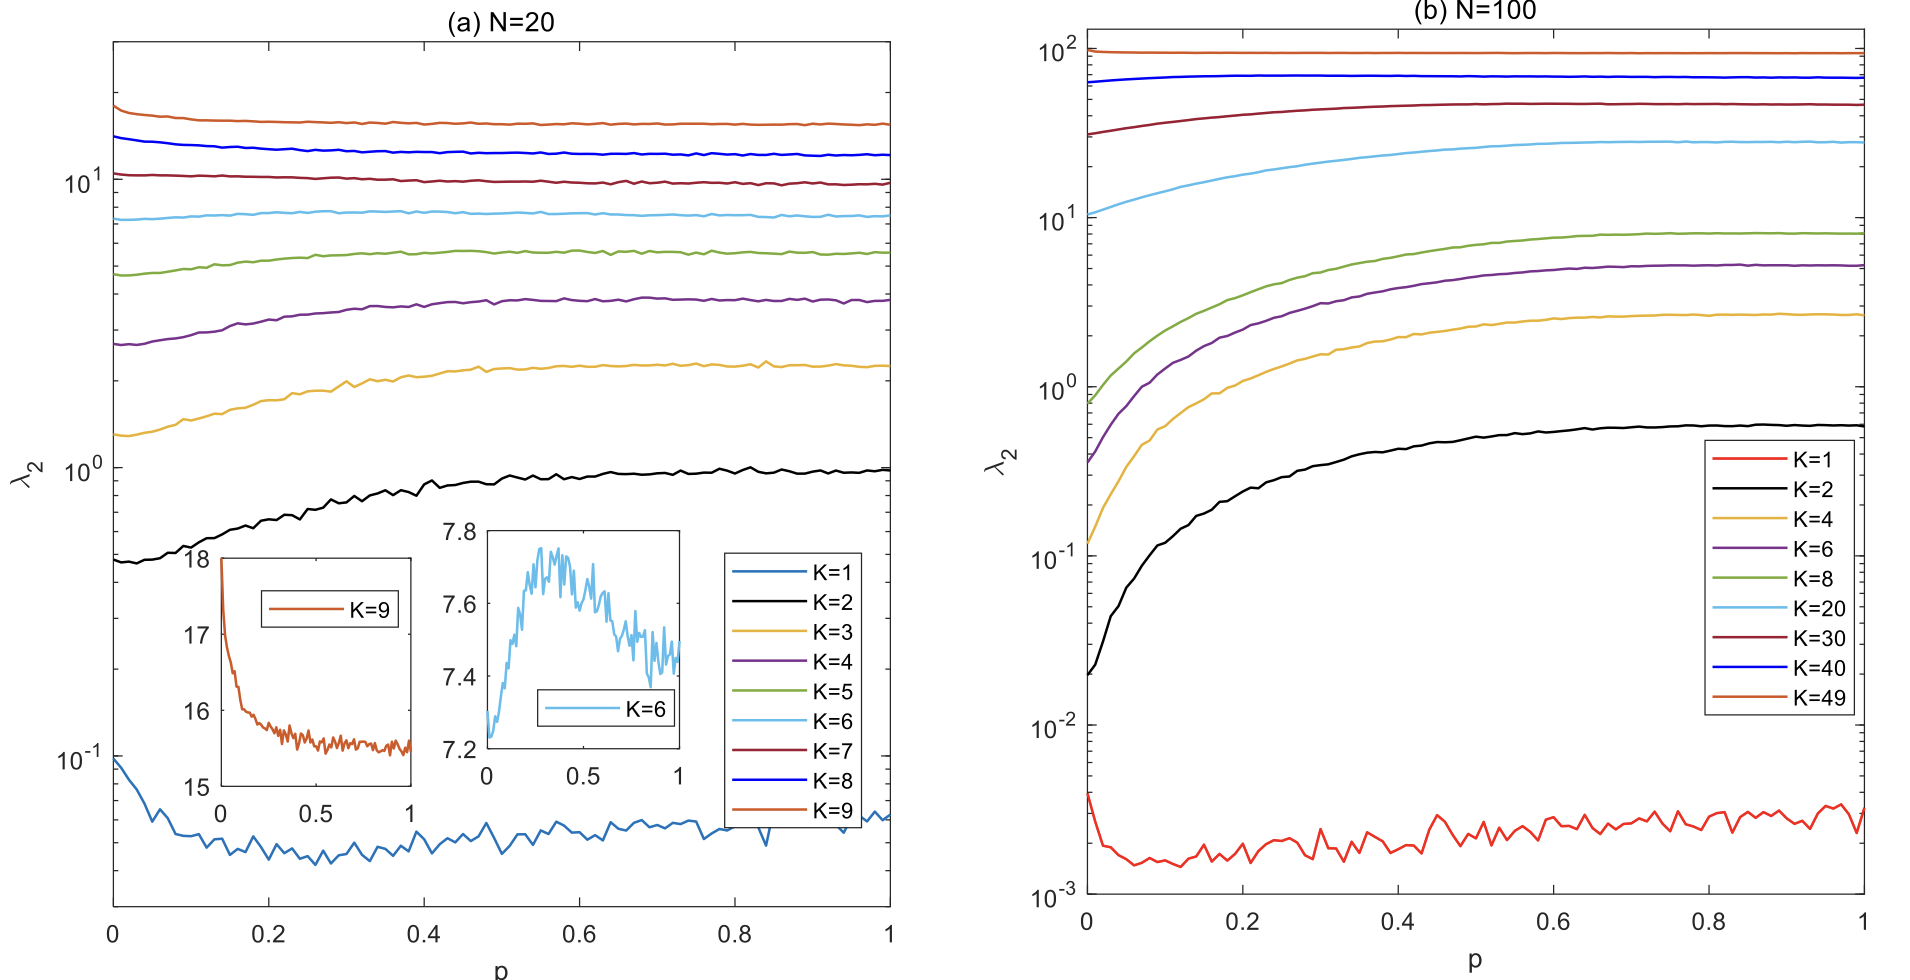
\includegraphics[width=\textwidth]{tb2.png}
    \caption{第二大特征值与重连概率的关系}
\end{figure}
下图则给出了粒子个数为 $\mathrm{N}=20,100$ 时, Duffing-WS小世界网络 Laplacian 矩阵的最大特征值 $\lambda_N$在不同的 $\mathrm{K}$ 值下随重连概率 $\mathrm{p}$
变化的曲线(平均 100次)。可以看出,在$N=20$时,最大特征值随着重连概率的增加而增大,连接度越大则最大特征值越大。在$N=100$时
,连接度小于40时随着重连概率的增大最大特征值增大,但是在连接度为40时发生突变,形成先下降后增加的趋势,随后变化不明显。
\begin{figure}[!htbp]
    \centering
    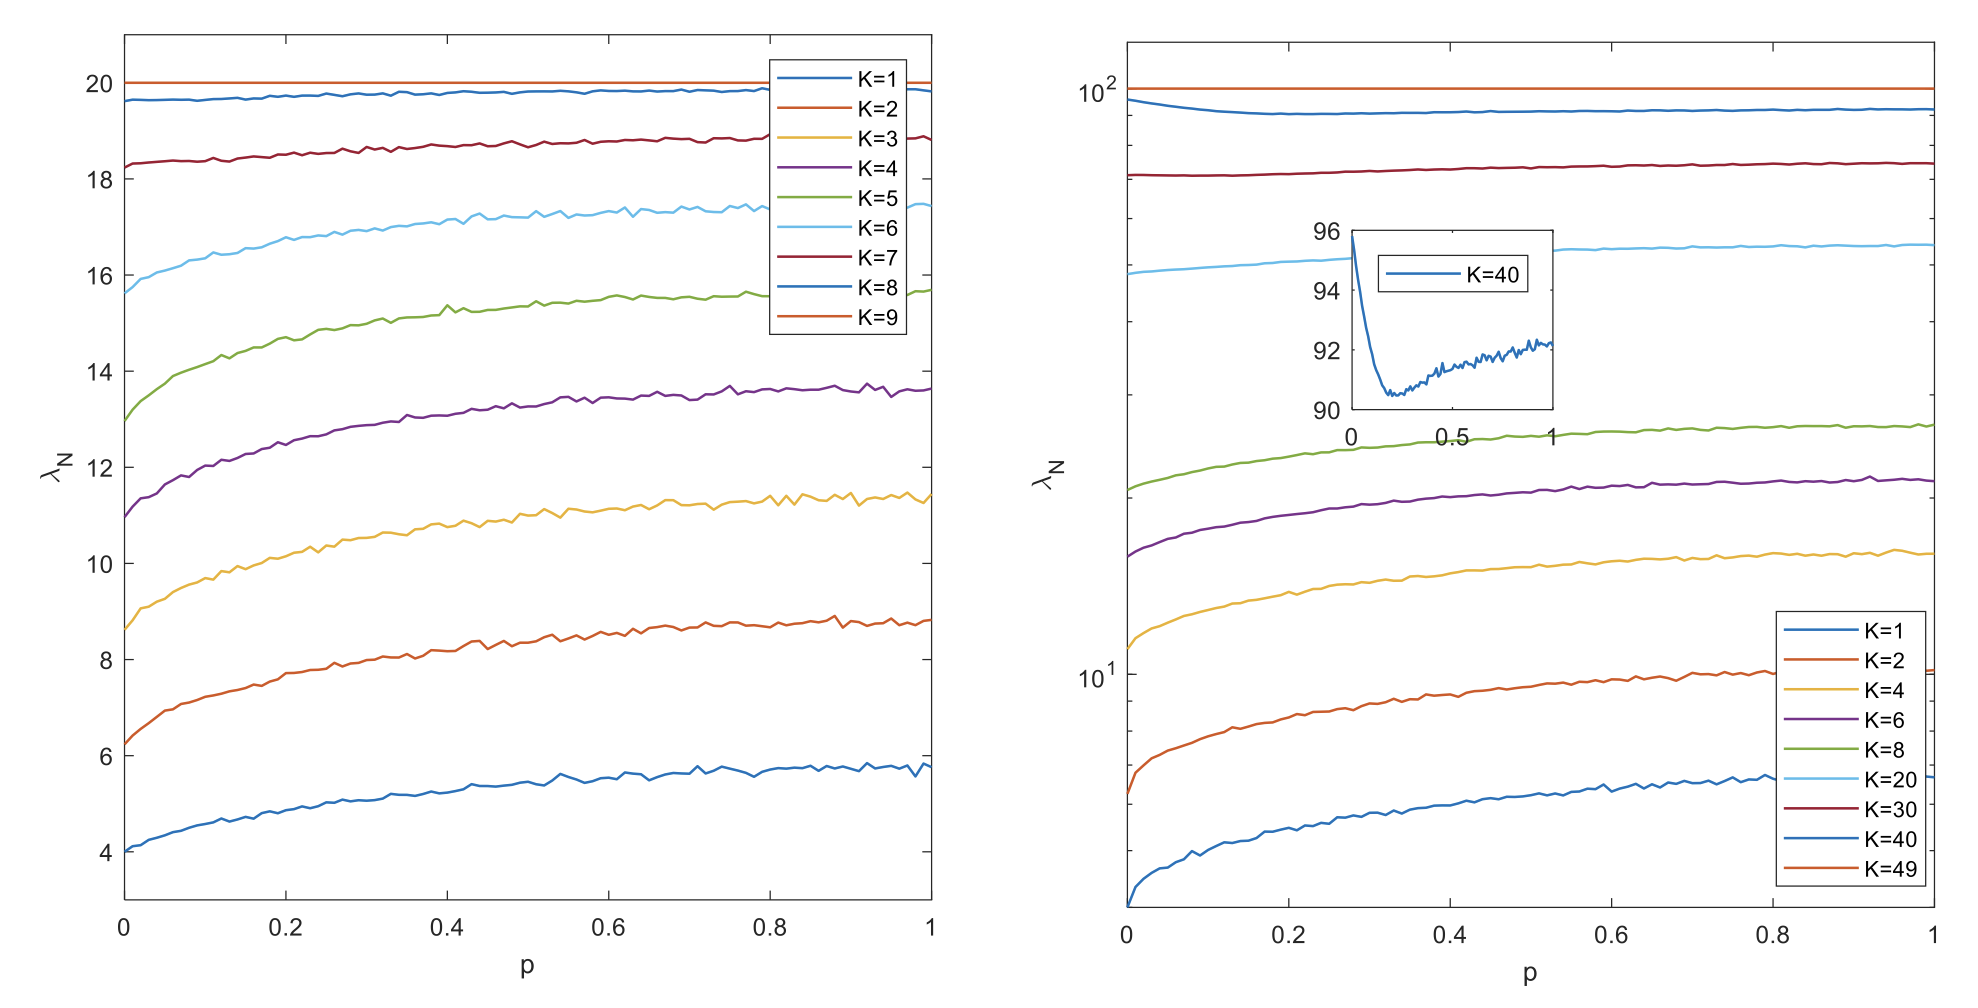
\includegraphics[width=\textwidth]{tb3.png}
    \caption{最大特征值与重连概率的关系}
\end{figure}
\section{小结} 
本文基于经典的Duffing振子,提出了一个以WS小世界网络方式进行连接的Duffing型复杂网络
(简称Duffing-WS型小世界网络),利用变分法推导该网络的最大李雅普诺夫指数表达式,
以庞加莱截面分岔图和李雅普诺夫指数为工具研究其混沌现象,并分析小世界网络重连度,
重连概率和耦合强度等参数对其混沌运动状态参数范围的影响。研究表明,Duffing-WS小世界网络的各
个粒子输出也呈现出小尺度周期运动、倍周期分岔、混沌和大尺度周期运动等多种状态,
其混沌的参数范围较单个Duffing方程更为复杂。网络重连度,重连概率和耦合强度等参数对其混
沌区域的影响也较传统规则网络有明显不同。
\chapter{混沌信号的稀疏重构算法}
在实际情况下,混沌信号总会被噪声污染,又由于混沌信号的非周期、宽带频谱等特性,使得一些现有的信号重构方法在处理混沌信号时难以获得理想的效果。
为此,本章基于稀疏重构理论提出了一种针对被噪声污染混沌信号的重构算法,而随后的以第3章提出的Duffing-WS小世界网络输出混沌信号为例的仿真实验也表明,该方法能较为稳健地恢复受噪声干扰的Duffing-WS型小世界网络输出的带噪混沌信号,不仅较具有更高的输出信噪比, 而原始信号的混沌特性也能得到较大程度的恢复,这是一般稀疏重构算法不具有的。

\section{基于稀疏重构的混沌信号重构算法}
设Duffing-WS小世界网络(*)某个节点输出的离散化带噪混沌信号序列为:
\begin{equation}
    u[n]=x[n]+w[n], n=1,2, \ldots, N
\end{equation}
其中 $x[n]$ 为原始混沌序列, $w[n]$ 为零均值和方差为 $\sigma$ 的高斯白噪声。因此,方程(*)又写成矢量形式为:
\begin{equation}
    \boldsymbol{u}=\boldsymbol{x}+\boldsymbol{w}
\end{equation}

我们知道 Duffing-WS 小世界网络输出的混沌信号在时域上并不是稀疏信号,
但它可能具有某类特定的变换基 $\Psi$, 使得在此基上的变换系数服从幂指数递减,
这也说明该信号在此变换域中具有较强的可压缩性。
这里不妨假设 $\boldsymbol{x}=\Psi \boldsymbol{a}, \boldsymbol{a}$ 为稀疏表示系数,
我们保留所有系数中绝对值最大的 $s$ 个系数得到 真正的稀疏系数 $\hat{\boldsymbol{a}}_s$,
基于稀疏重构理论的混沌信号重构问题便是需要求解如下 的 基于$l_1$ 范数的稀疏重构最优化问题:
\begin{equation}
    \min \left\|\hat{\boldsymbol{a}}_s\right\|_1, \text { s.t., }\left\|\Psi \hat{\boldsymbol{a}}_s-\boldsymbol{y}\right\|_2 \leq \boldsymbol{\varepsilon}
\end{equation}\par
我们知道,基于$l_1$范数的稀疏重构算法有利于保持信号的稀疏性,也称为基追踪算法。目前针对该问题的重构算法主要可归为凸优化算法、贪婪算法和
组合算法三大类。其中,贪婪算法通过每次迭代时选择一个局部最优解来逐步逼近原始信号,简单、易于理解且快速方便。
典型的贪婪算法有匹配追踪(MP)算法,而改进的有正交匹配追踪(OMP)算法和压缩采样匹配追踪(CoSaMP)算法等。
压缩采样匹配追踪(CoSaMP)算法是由Needell与Tropp提出的一个针对OMP的改进算法,具有比MP和OMP更好的数值表现,
该算法是结合OMP思想与采样技巧,在每次迭代中将一些随机样本加入到选定的支撑集中,并采用最小二乘法对所选支撑集进行解的估计。

本章考虑基于 CoSaMP 算法对带噪的混沌信号进行重构, 其中而稀疏变换基 选择离散傅里叶变换基。这是因为混沌信号虽然具有时域类随机性但它认可看成低频信号,因此其傅里叶系数在高频区域将大幅度衰减,因此我们可将其高频傅里叶系数置零将其离散信号转换为近似稀疏向量。

算法的输入为采样矩阵 $\boldsymbol{\Phi}$ (这里设置为高斯随机矩阵)和 采样信号 $\boldsymbol{u}$
(即 Duffing-WS小世界网络某个节点输出的带噪混沌信号), 并假设采样信号截断处理后的傅里叶基表示系数 $\boldsymbol{a}$
的稀疏度为 $s$; 算法的输出为 $s$ 维的 压缩后的信号 $\boldsymbol{a}$, 利用傅里叶逆变换即可重构原始混沌信号。


\section{仿真分析}
这一节我们给出用OMP和CoSaMP两种稀疏重构算法对混沌信号的稀疏采样后还原的仿真结果对比和分析,其中混沌信号选择为模型
Duffing-WS小世界网络第一个节点的输出,并叠加一定强度的高斯白噪声。\par
\begin{figure}[!htbp]
    \centering
    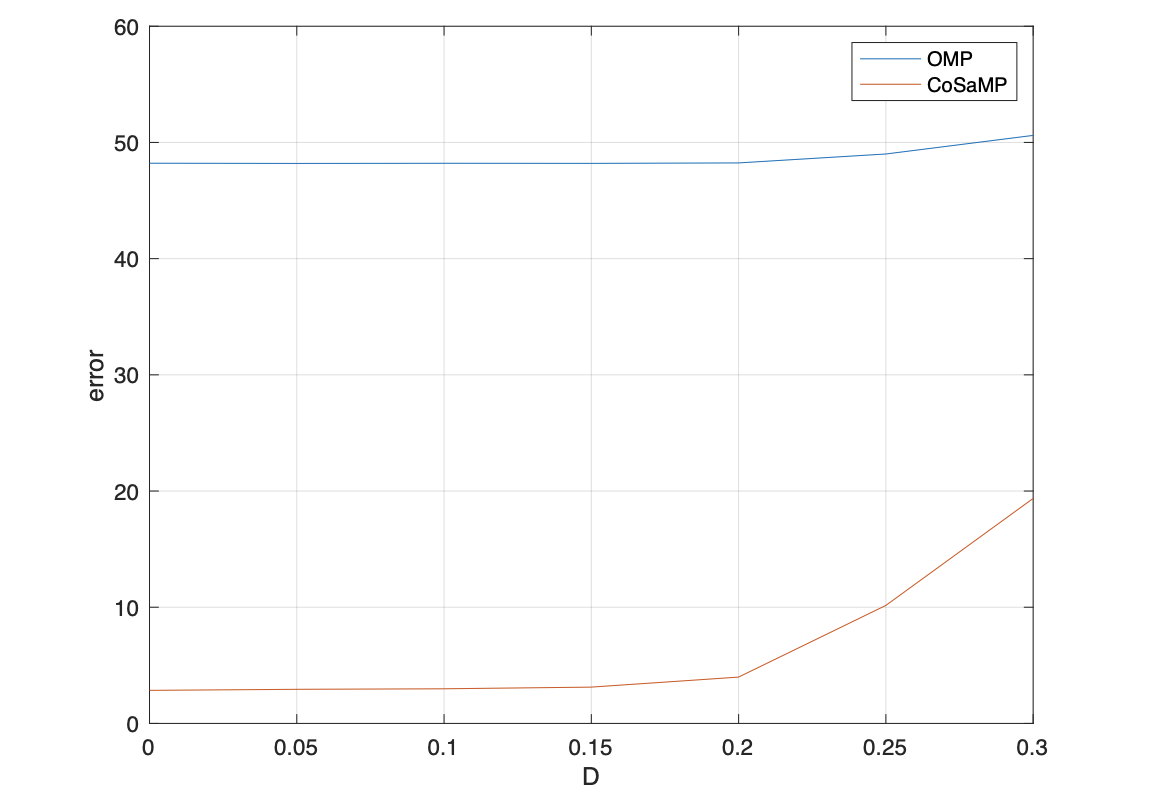
\includegraphics[width=0.7\textwidth]{42.png}
\end{figure}
图(*)给出了OMP和CoSaMP两种算法的重构误差关于噪声强度的变化图,其中重构误差定义为重构输出信号和真实信号差的$l_2$范数。可以看到,CoSaMP算法在噪声强度小于0.2时具有非常低的重构误差,
即较好的抗噪重构性能,但之后因噪声强度的增加其误差有快速增长,但其重构性能始终优于经典的OMP算法。
经典的OMP算法对于混沌信号始终存在较大的重构误差。由此可见,CoSaMP算法相较于传统OMP算法有更出色的重构抗噪声能力。\par
\begin{figure}[!htbp]
    \centering
    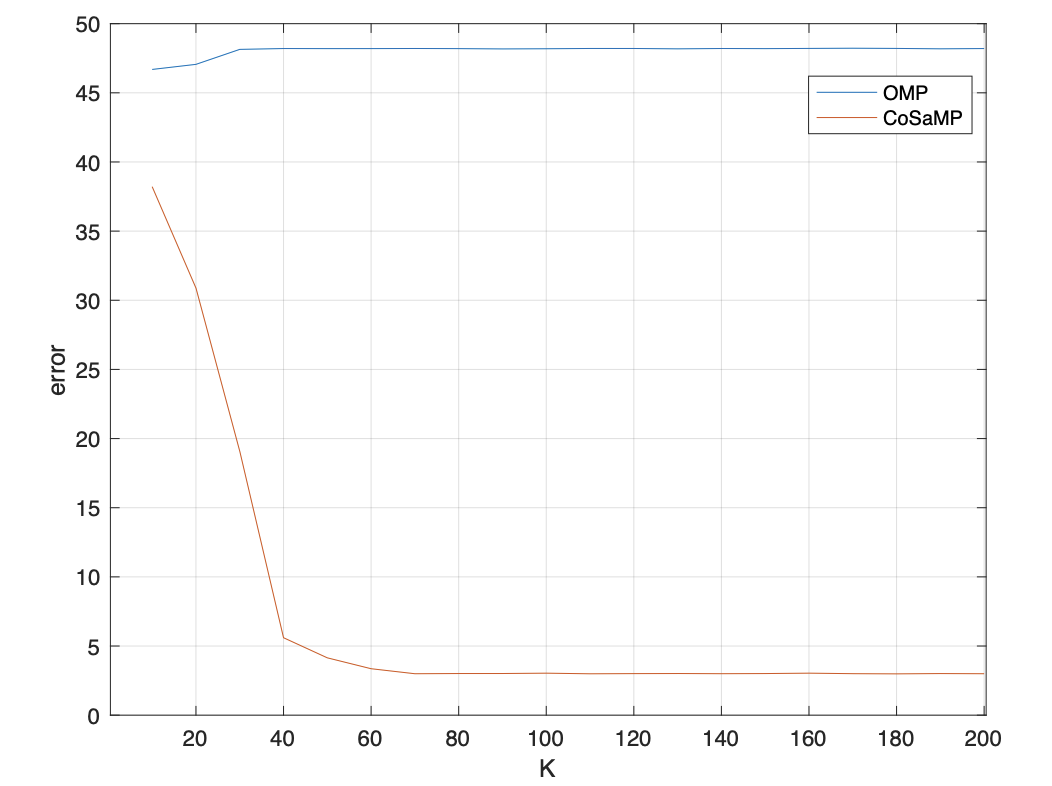
\includegraphics[width=0.7\textwidth]{43.png}
\end{figure}

图(*)则给出了选择不同稀疏度$K$值时,OMP和CoSaMP两种算法相应的重构误差。可以看出,CoSaMP算法在稀疏度增加时重构误差显著减小,
在$K = 60$左右趋于稳定,也说明该混沌信号经过离散傅里叶变换之后的稀疏系数取为$K = 60$即可较为稳健地恢复该信号,
而OMP算法对该混沌信号的重构能力一直不佳。\par
由此可见,含噪声的混沌信号稀疏重构问题目前尚未有完善的研究,常规的稀疏重构算法也对混沌信号的重构性能不佳,
以OMP算法为例,该算法在常规情况有很好的性能,但是在混沌信号情形的效果不佳。因此对混沌信号重构对传统稀疏重构算法提出了新的挑战。
\section{小结}
混沌信号作为复杂网络常见的输出形式,构建相应混沌信号在噪声干扰下的重构方法,对复杂网络的混沌控制和混沌信号的各种应用都具有重要的意义。
本章针对复杂网络输出的混沌信号,运用稀疏采样还原算法成功压缩且高精度还原了带噪声的混沌信号,并且对比了不同算法和在混沌信号情形下的性能。
仿真实验表明, 该方法能较为稳健地恢复受噪声干扰的Duffing-WS型小世界网络输出的带噪混沌信号,不仅较具有更高的输出信噪比, 而原始信号的混沌特性也能得到较大程度的恢复,
这是一般稀疏重构算法不具有的。
\chapter{结论}
复杂网络广泛存在于各个科学领域,对复杂网络的研究目前已成为非线性科学和复杂性问题领域的一个研究热点。复杂网络的各个节点具有自身的动力学,而这些节点由于网络拓扑结构的不同而演化出不同的群体行为,可能收敛于平衡点、周期轨或者混沌吸引子。混沌作为复杂网络重要的动力学特性,研究其产生机理和对参数的依赖性,构建相应混沌信号在噪声干扰下的重构方法,对复杂网络的混沌控制和混沌信号的各种应用都具有重要的意义。
\par 本文生成一种新的Duffing-WS型小世界网络模型,通过变分法计算出其最大李雅普诺夫指数表达式作为衡量网络混沌的标准,分析不同参数对网络混沌的影响。同时运用稀疏采样还原算法成功压缩且高精度还原了带噪声的混沌信号,并且对比了不同算法和在混沌信号情形下的性能。
我们发现,Duffing-WS小世界网络具有比单个Duffing-方程更为复杂的混沌特性,而系统重连概率、重连度以及耦合强度对系统混沌区域的影响也有别于传统规则网络:
和传统的规则网络不同,网络耦合强度$\varepsilon$对混沌的影响并不是单调的,当网络重连度K较小时,耦合强度的增强反而会促进系统的混沌现象;只有在重连度K增大到一定程度之后,较强的耦合强度才会对系统混沌起到控制效果;但是重连度K足够大以后,系统混沌
网络重连度K在不同重连概率p下对混沌有明显的影响,对于规则网络(p = 0)和小世界网络(0< p <1),足够大的重连度会抑制系统混沌,较小的重连度则促进系统的混沌运动;相比前面两种网络,完全随机网络(p = 1)的混沌区域则更大,重连度K对其混沌区域的影响也呈现非单调性,随着重连度K的增加,其混沌区域先增加后减小。
网络重连概率p对复杂网络混沌区域的影响不明显。\par
本文同时对小世界网络模型的同步性进行了初步研究,给出了重连概率与网络同步性的分析。最后本文针对混沌信号进行稀疏重构算法的适应性研究,得出混沌信号对
两种算法的适应性分析。
%---------------------------------------------------------------------------%
% main content
%-
%-> Appendix
%-
\cleardoublepage%
\appendix% initialize the environment
%\chapter{中国科学院大学学位论文撰写要求}

学位论文是研究生科研工作成果的集中体现,是评判学位申请者学术水平、授予其学位的主要依据,是科研领域重要的文献资料。根据《科学技术报告、学位论文和学术论文的编写格式》(GB/T 7713-1987)、《学位论文编写规则》(GB/T 7713.1-2006)和《文后参考文献著录规则》(GB7714—87)等国家有关标准,结合中国科学院大学(以下简称“国科大”)的实际情况,特制订本规定。

\section{论文无附录者无需附录部分}

\section{测试公式编号 \texorpdfstring{$\Lambda,\lambda,\theta,\bar{\Lambda},\sqrt{S_{NN}}$}{$\textLambda,\textlambda,\texttheta,\bar{\textLambda},\sqrt{S_{NN}}$}} \label{sec:testmath}

\begin{equation} \label{eq:appedns}
    \adddotsbeforeeqnnum%
    \begin{cases}
        \frac{\partial \rho}{\partial t} + \nabla\cdot(\rho\Vector{V}) = 0\\
        \frac{\partial (\rho\Vector{V})}{\partial t} + \nabla\cdot(\rho\Vector{V}\Vector{V}) = \nabla\cdot\Tensor{\sigma}\\
        \frac{\partial (\rho E)}{\partial t} + \nabla\cdot(\rho E\Vector{V}) = \nabla\cdot(k\nabla T) + \nabla\cdot(\Tensor{\sigma}\cdot\Vector{V})
    \end{cases}
\end{equation}
\begin{equation}
    \adddotsbeforeeqnnum%
    \frac{\partial }{\partial t}\int\limits_{\Omega} u \, \mathrm{d}\Omega + \int\limits_{S} \unitVector{n}\cdot(u\Vector{V}) \, \mathrm{d}S = \dot{\phi}
\end{equation}
\[
    \begin{split}
        \mathcal{L} \{f\}(s) &= \int _{0^{-}}^{\infty} f(t) e^{-st} \, \mathrm{d}t, \ 
        \mathscr{L} \{f\}(s) = \int _{0^{-}}^{\infty} f(t) e^{-st} \, \mathrm{d}t\\
        \mathcal{F} {\bigl (} f(x+x_{0}) {\bigr )} &= \mathcal{F} {\bigl (} f(x) {\bigr )} e^{2\pi i\xi x_{0}}, \ 
        \mathscr{F} {\bigl (} f(x+x_{0}) {\bigr )} = \mathscr{F} {\bigl (} f(x) {\bigr )} e^{2\pi i\xi x_{0}}
    \end{split}
\]

mathtext: $A,F,L,2,3,5,\sigma$, mathnormal: $A,F,L,2,3,5,\sigma$, mathrm: $\mathrm{A,F,L,2,3,5,\sigma}$.

mathbf: $\mathbf{A,F,L,2,3,5,\sigma}$, mathit: $\mathit{A,F,L,2,3,5,\sigma}$, mathsf: $\mathsf{A,F,L,2,3,5,\sigma}$.

mathtt: $\mathtt{A,F,L,2,3,5,\sigma}$, mathfrak: $\mathfrak{A,F,L,2,3,5,\sigma}$, mathbb: $\mathbb{A,F,L,2,3,5,\sigma}$.

mathcal: $\mathcal{A,F,L,2,3,5,\sigma}$, mathscr: $\mathscr{A,F,L,2,3,5,\sigma}$, boldsymbol: $\boldsymbol{A,F,L,2,3,5,\sigma}$.

vector: $\Vector{\sigma, T, a, F, n}$, unitvector: $\unitVector{\sigma, T, a, F, n}$

matrix: $\Matrix{\sigma, T, a, F, n}$, unitmatrix: $\unitMatrix{\sigma, T, a, F, n}$

tensor: $\Tensor{\sigma, T, a, F, n}$, unittensor: $\unitTensor{\sigma, T, a, F, n}$ 

\section{测试生僻字}

霜蟾盥薇曜灵霜颸妙鬘虚霩淩澌菀枯菡萏泬寥窅冥毰毸濩落霅霅便嬛岧峣瀺灂姽婳愔嫕飒纚棽俪緸冤莩甲摛藻卮言倥侗椒觞期颐夜阑彬蔚倥偬澄廓簪缨陟遐迤逦缥缃鹣鲽憯懔闺闼璀错媕婀噌吰澒洞阛闠覼缕玓瓑逡巡諓諓琭琭瀌瀌踽踽叆叇氤氲瓠犀流眄蹀躞赟嬛茕頔璎珞螓首蘅皋惏悷缱绻昶皴皱颟顸愀然菡萏卑陬纯懿犇麤掱暒 墌墍墎墏墐墒墒墓墔墕墖墘墖墚墛坠墝增墠墡墢墣墤墥墦墧墨墩墪樽墬墭堕墯墰墱墲坟墴墵垯墷墸墹墺墙墼墽垦墿壀壁壂壃壄壅壆坛壈壉壊垱壌壍埙壏壐壑壒压壔壕壖壗垒圹垆壛壜壝垄壠壡坜壣壤壥壦壧壨坝塆圭嫶嫷嫸嫹嫺娴嫼嫽嫾婳妫嬁嬂嬃嬄嬅嬆嬇娆嬉嬊娇嬍嬎嬏嬐嬑嬒嬓嬔嬕嬖嬗嬘嫱嬚嬛嬜嬞嬟嬠嫒嬢嬣嬥嬦嬧嬨嬩嫔嬫嬬奶嬬嬮嬯婴嬱嬲嬳嬴嬵嬶嬷婶嬹嬺嬻嬼嬽嬾嬿孀孁孂娘孄孅孆孇孆孈孉孊娈孋孊孍孎孏嫫婿媚嵭嵮嵯嵰嵱嵲嵳嵴嵵嵶嵷嵸嵹嵺嵻嵼嵽嵾嵿嶀嵝嶂嶃崭嶅嶆岖嶈嶉嶊嶋嶌嶍嶎嶏嶐嶑嶒嶓嵚嶕嶖嶘嶙嶚嶛嶜嶝嶞嶟峤嶡峣嶣嶤嶥嶦峄峃嶩嶪嶫嶬嶭崄嶯嶰嶱嶲嶳岙嶵嶶嶷嵘嶹岭嶻屿岳帋巀巁巂巃巄巅巆巇巈巉巊岿巌巍巎巏巐巑峦巓巅巕岩巗巘巙巚帠帡帢帣帤帨帩帪帬帯帰帱帲帴帵帷帹帺帻帼帽帾帿幁幂帏幄幅幆幇幈幉幊幋幌幍幎幏幐幑幒幓幖幙幚幛幜幝幞帜幠幡幢幤幥幦幧幨幩幪幭幮幯幰幱庍庎庑庖庘庛庝庠庡庢庣庤庥庨庩庪庬庮庯庰庱庲庳庴庵庹庺庻庼庽庿廀厕廃厩廅廆廇廋廌廍庼廏廐廑廒廔廕廖廗廘廙廛廜廞庑廤廥廦廧廨廭廮廯廰痈廲廵廸廹廻廼廽廿弁弅弆弇弉弖弙弚弜弝弞弡弢弣弤弨弩弪弫弬弭弮弰弲弪弴弶弸弻弼弽弿彖彗彘彚彛彜彝彞彟彴彵彶彷彸役彺彻彽彾佛徂徃徆徇徉后徍徎徏径徒従徔徕徖徙徚徛徜徝从徟徕御徢徣徤徥徦徧徨复循徫旁徭微徯徰徱徲徳徴徵徶德徸彻徺忁忂惔愔忇忈忉忔忕忖忚忛応忝忞忟忪挣挦挧挨挩挪挫挬挭挮挰掇授掉掊掋掍掎掐掑排掓掔掕挜掚挂掜掝掞掟掠采探掣掤掦措掫掬掭掮掯掰掱掲掳掴掵掶掸掹掺掻掼掽掾掿拣揁揂揃揅揄揆揇揈揉揊揋揌揍揎揑揓揔揕揖揗揘揙揤揥揦揧揨揫捂揰揱揲揳援揵揶揷揸揻揼揾揿搀搁搂搃搄搅搇搈搉搊搋搌搎搏搐搑搒摓摔摕摖摗摙摚摛掼摝摞摠摡斫斩斮斱斲斳斴斵斶斸旪旫旮旯晒晓晔晕晖晗晘晙晛晜晞晟晠晡晰晣晤晥晦晧晪晫晬晭晰晱晲晳晴晵晷晸晹晻晼晽晾晿暀暁暂暃暄暅暆暇晕晖暊暋暌暍暎暏暐暑暒暓暔暕暖暗旸暙暚暛暜暝暞暟暠暡暣暤暥暦暧暨暩暪暬暭暮暯暰昵暲暳暴暵
% appendix content
%-
%-> Backmatter: bibliography, glossary, index
%-
\backmatter% initialize the environment
\intotoc*{\cleardoublepage}{\bibname}% add link to toc
\artxifstreq{\artxbib}{bibtex}{% enable bibtex
    \bibliography{Biblio/ref}% bibliography
}{%
    \printbibliography% bibliography
}
%---------------------------------------------------------------------------%
%->> Backmatter
%---------------------------------------------------------------------------%
\chapter[致谢]{致\quad 谢}\chaptermark{致\quad 谢}% syntax: \chapter[目录]{标题}\chaptermark{页眉}
%\thispagestyle{noheaderstyle}% 如果需要移除当前页的页眉
%\pagestyle{noheaderstyle}% 如果需要移除整章的页眉

感激casthesis作者吴凌云学长,gbt7714-bibtex-style
开发者zepinglee,和ctex众多开发者们。若没有他们的辛勤付出和非凡工作,\LaTeX{}菜鸟的我是无法完成此国科大学位论文\LaTeX{}模板ucasthesis的。在\LaTeX{}中的一点一滴的成长源于开源社区的众多优秀资料和教程,在此对所有\LaTeX{}社区的贡献者表示感谢!

ucasthesis国科大学位论文\LaTeX{}模板的最终成型离不开以霍明虹老师和丁云云老师为代表的国科大学位办公室老师们制定的官方指导文件和众多ucasthesis用户的热心测试和耐心反馈,在此对他们的认真付出表示感谢。特别对国科大的赵永明同学的众多有效反馈意见和建议表示感谢,对国科大本科部的陆晴老师和本科部学位办的丁云云老师的细致审核和建议表示感谢。谢谢大家的共同努力和支持,让ucasthesis为国科大学子使用\LaTeX{}撰写学位论文提供便利和高效这一目标成为可能。



\cleardoublepage[plain]% 让文档总是结束于偶数页,可根据需要设定页眉页脚样式,如 [noheaderstyle]
%---------------------------------------------------------------------------%
% other information
\end{document}
%---------------------------------------------------------------------------%

